\documentclass[nonacm,sigconf]{acmart}
\usepackage{graphicx}
\usepackage{subcaption}
\makeatletter
\@ifclasswith{acmart}{nonacm}{
  \settopmatter{printacmref=false} % Removes citation information below abstract
  \renewcommand\footnotetextcopyrightpermission{} % Removes footnote with conference information
  \fancyhead{} % Clears all header fields
  \fancyfoot{} % Clears all footer fields
  \fancyhead[L]{\shorttitle} % Optional: Add short title to left header
  \fancyhead[R]{\shortauthors} % Optional: Add short authors to right header
  \fancyfoot[C]{\thepage} % Optional: Page number in center footer
  % \AtBeginDocument{The pagesize is \texttt{a5paper}.\par}
}{}
\makeatother
\begin{document}

\title{Anomaly Detection in ECG Using LSTM and Autoencoder}


\author{Niaz Rahman}
\affiliation{%
  \institution{1905046}
  \city{Computer Science and Engineering}
  \country{Bangladesh University of Engineering and Technology}
}

\author{Asif Al Shahriar}
\affiliation{%
  \institution{1905040}
  \city{Computer Science and Engineering}
  \country{Bangladesh University of Engineering and Technology}
}

\maketitle

\section{Introduction}
\subsection{Problem Definition}
Cardiovascular diseases remain a leading cause of death worldwide, and early
detection is crucial for effective management and treatment. The project’s
goal is to create a system that tracks heart activity and alerts of any irregularities. The project addresses a real-time, automated, and reliable solution
using time series analysis and identification of irregular patterns in sequential
data of heart.

\subsection{Literature Review}
We have found two papers related to our problem.
\subsubsection{\textbf{Base  Paper: ECG-NET: A deep LSTM autoencoder for detecting anomalous ECG}}
This paper uses LSTM autoencoder to detect anomalous ECG.The encoder part encodes the ECG signal into a lower dimensional latent space representation and decoder part then tries to reconstruct the specified ECG signal. The model is trained only on normal (non-anomalous) ECG signals. Then reconstruction loss of test ECG signals are calculated. Next a reconstruction loss threshold value is determined from the frequency distribution of the reconstruction losses so that from the reconstruction loss value above a certain threshold is determined as anomaly, otherwise it will be treated as normal.\cite{roy2023ecg}

The proposed model achieved more than 0.98 accuracy having precision, recall and F1 values more than 0.94, 0.97, 0.96 respectively.

\subsubsection{\textbf{State of The Art : Unsupervised Transformer-Based Anomaly Detection in ECG Signals}}
This paper is a very recent work similar to our problem. It uses a Transformer based model for anomaly detection in ECG.This model uses unsupervised learning. The overall model architecture comprises two parts: an embedding layer and a standard transformer encoder. All normal time series data of ECG signals, which take the form of a 2D tensor of sequence length × number of features, were first encoded into sequences of embeddings, which were then fed into a multilayer bidirectional transformer network to produce their corresponding representations. The final linear dense layers predicted the input ECG signal with the same input sequence length.\cite{alamr2023unsupervised}

The model can detect anomalies with 0.99 accuracy, 0.99 F1-score, 0.981 recall, and 1.0 precision.

\subsection{Research Gap}
Despite the progress made in utilizing deep learning for ECG anomaly detection, several gaps remain in the current literature. Many existing models either require labeled datasets for training or struggle with generalization across diverse patient populations and varying signal qualities. Additionally, while some approaches focus on specific types of anomalies, there is a lack of comprehensive models capable of detecting a broad spectrum of irregularities within ECG signals. This project seeks to address these gaps by developing an LSTM-Autoencoder model that not only enhances real-time anomaly detection but also improves generalization capabilities across different datasets. By focusing on both common and rare anomalies, this research aims to contribute significantly to the field of cardiac health monitoring and diagnostics.

\section{Materials and Methods}
\subsection{Dataset}
We have worked on two datasets.
\subsubsection{\textbf{ECG5000}}
The dataset consists of 5,000 ECG recordings, each containing 140 data points, representing a total duration of 20 hours. Each heartbeat has been extracted and standardized to equal length through interpolation. The labels in this dataset are binary, with 0 indicating an abnormal heartbeat and 1 indicating a normal heartbeat.The dataset can be found 
\href{http://storage.googleapis.com/download.tensorflow.org/data/ecg.csv}{\textcolor{blue}{here}}.

\begin{figure}[h]
  \centering
  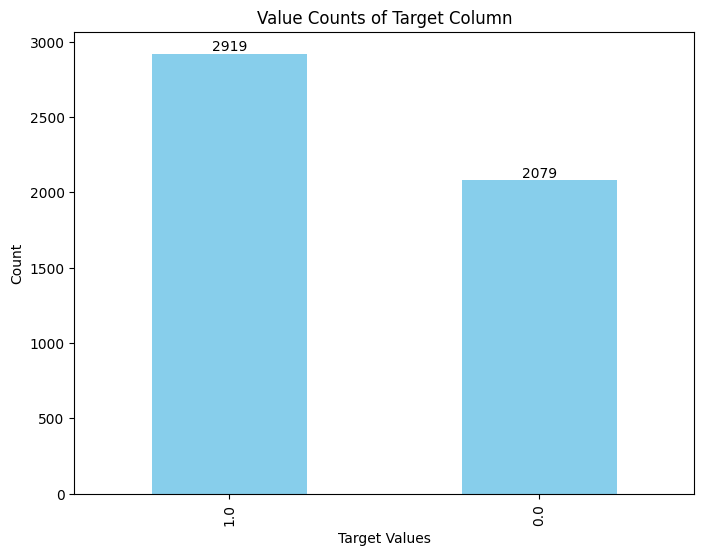
\includegraphics[width=0.3\textwidth]{ecg5000/binary.png}
  \caption{No of samples for each Binary Class}
  \Description{No of samples for each Binary Class}
\end{figure}

\subsubsection{\textbf{MIT-BIH}}
The dataset comprises raw ECG signals, featuring 48 half-hour excerpts of two-channel ECG recordings. It includes five distinct classes: N for normal readings, and A, L, R, and V for abnormal readings. The database contains several file types: .atr files provide rhythmic annotations, .dat files contain the actual ECG data and .hea files offer additional header information.The dataset can be found 
\href{https://physionet.org/content/mitdb/1.0.0/}{\textcolor{blue}{here}}.


Our Model is focused on ECG5000 Dataset. To work on MIT-BIH Dataset, we need to interpolate in the same way ECG5000 has been extracted and interpolated. Interpolation Technique\cite{castiglioni2003interpolation} for MIT-BIH:
\begin{enumerate}
\item  Input ECG Signal: 
   \[
   \text{ECG}_{in}(t)
   \]

\item  Identify QRS Complex: 
   \[
   \text{QRS}_{complex} = f(\text{ECG}_{in}(t))
   \]

\item  Determine R Peak (\(t_R\)): 
   \[
   t_R = \arg\max(\text{QRS}_{complex})
   \]

\item  Zero-Padding: 
   \[
   \text{ECG}_{padded}(t) = 
   \begin{cases} 
   \text{ECG}_{in}(t) & t < t_R \\ 
   0 & t \geq t_R + T_{pad} 
   \end{cases}
   \]

\item  Compute Discrete Fourier Transform (DFT): 
   \[
   X(f) = DFT(\text{ECG}_{padded}(t))
   \]

\item  Inverse Discrete Fourier Transform (IDFT): 
   \[
   \text{ECG}_{reconstructed}(t) = IDFT(X(f))
   \]

\item  Extract Area of QRS Complex (\(A_{QRS}\)): 
   \[
   A_{QRS} = \int_{t_{start}}^{t_{end}} |\text{ECG}_{reconstructed}(t)| dt
   \]

\item  Output Features: 
    \(A_{QRS}\),
    \(t_R\),
    Other relevant features
\end{enumerate}
After using this interpolation method, we can use our model on MIT-BIH Dataset as well as ECG5000.
\subsection{Proposed Architecture}
The procedure of our proposed architecture is as follows:
\begin{figure}[h]
  \centering
  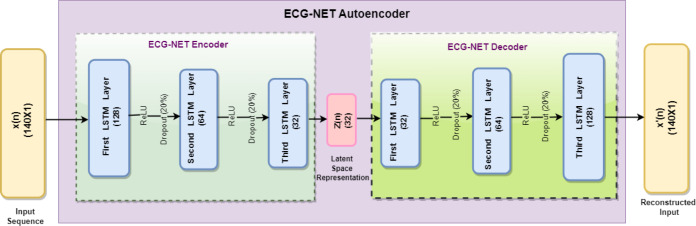
\includegraphics[width=0.5\textwidth]{LSTMs/ecgnet.png}
  \caption{Proposed Architecture}
  \Description{Proposed Architecture}
\end{figure}
\begin{enumerate}
    \item \textbf{Data Preparation and Preprocessing}: This step includes normalizing the data, segmenting it into readable sequences and ensuring that the data is free from noises.

    \item \textbf{Model Architecture}: We have used the LSTMs to process time-series data effectively and Autoencoder to detect anomaly in time series data. Autoencoder has two stage. Encoding stage compresses the input data into a condensed representation. Decoding Stage reconstruct the data from representation.

    \item \textbf{Training the Model} 
    The model is trained with normal ECG data so that it learns the baseline of what constitutes a normal hearth rythm.Training Loss is also computed.

    \item \textbf{Validation and Setting Threshold}
    The parameters like learning rate, number of layers are tuned using validation set which also consists of normal ECG data.Validation loss is computed and later threshold is selected from the loss.

    \item {\textbf{Testing and Classification}}
    The Model is tested with both normal and abnormal ECG data. Then reconstruction loss is computed.If reconstruction losses are greater than threshold, then the data is anomalous. Otherwise, the data is normal.
\end{enumerate}

\subsection{LSTM Variations}
We have tried different LSTM architectures.
\subsubsection{\textbf{Stacked LSTM}}
Stacked LSTMs consist of multiple LSTM layers stacked on top of each other, enhancing the model's ability to learn complex patterns in sequential data. Each layer captures different levels of abstraction, with lower layers focusing on simple features and higher layers on more complex relationships. This hierarchical structure improves performance in tasks such as natural language processing and time-series prediction by enabling deeper feature extraction. The increased capacity allows for better generalization on unseen data, making stacked LSTMs a powerful tool in deep learning applications.
\begin{figure}[h]
  \centering
  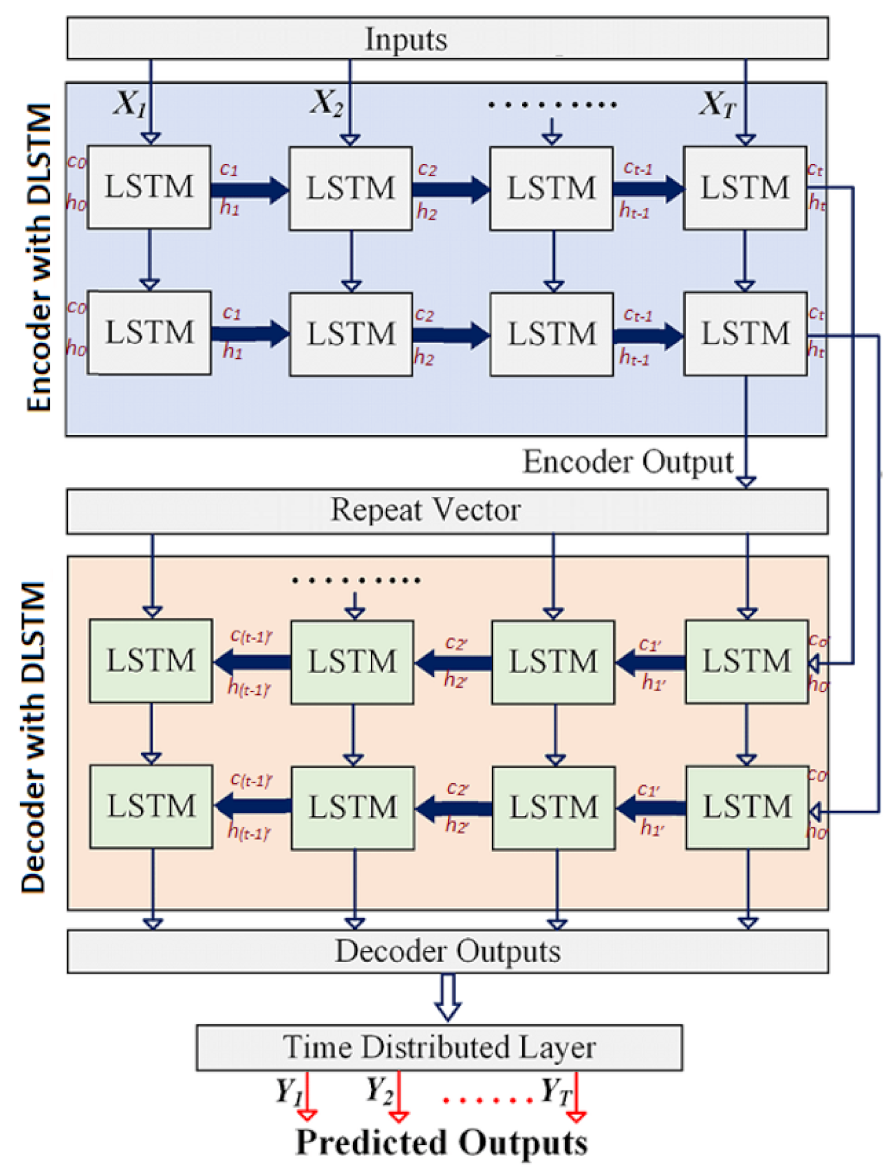
\includegraphics[width=0.5\textwidth]{LSTMs/stacked.png}
  \caption{Stacked LSTM}
  \Description{Stacked LSTM}
\end{figure}

\subsubsection{\textbf{CNN LSTM}}
CNN-LSTM combines Convolutional Neural Networks (CNNs) with Long Short-Term Memory (LSTM) networks to leverage the strengths of both architectures. CNNs are effective at extracting spatial features from data, such as images or video frames, while LSTMs excel at capturing temporal dependencies in sequences. This hybrid approach is particularly useful in applications like video classification or activity recognition, where spatial and temporal information are crucial. By first applying CNN layers to extract features and then feeding these into LSTM layers, the model can effectively learn from both the spatial and sequential dimensions of the data.
\begin{figure}[h]
  \centering
  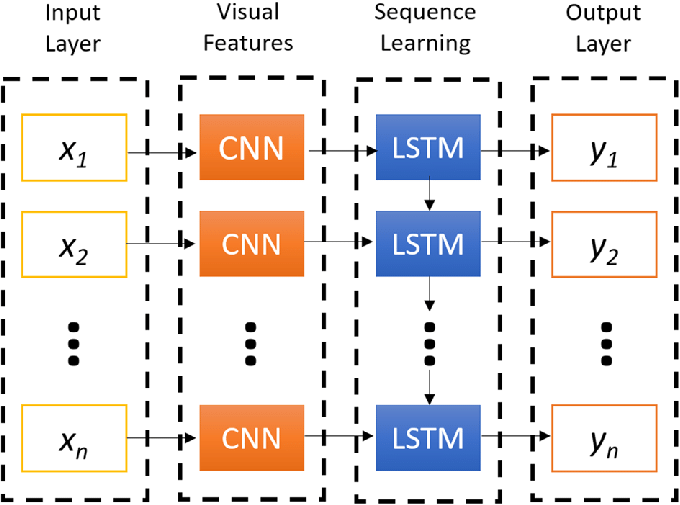
\includegraphics[width=0.5\textwidth]{LSTMs/cnn.png}
  \caption{CNN LSTM}
  \Description{CNN LSTM}
\end{figure}

\subsubsection{\textbf{Bidirectional LSTM}}
Bidirectional LSTMs enhance standard LSTMs by processing input sequences in both forward and backward directions. This architecture allows the model to capture context from both past and future states, improving its understanding of the sequence as a whole. Bidirectional LSTMs are particularly beneficial in tasks such as sentiment analysis or machine translation, where context from both directions can significantly impact the output. By combining outputs from both directions, these models achieve better performance compared to unidirectional LSTMs, especially in complex language tasks.
\begin{figure}[h]
  \centering
  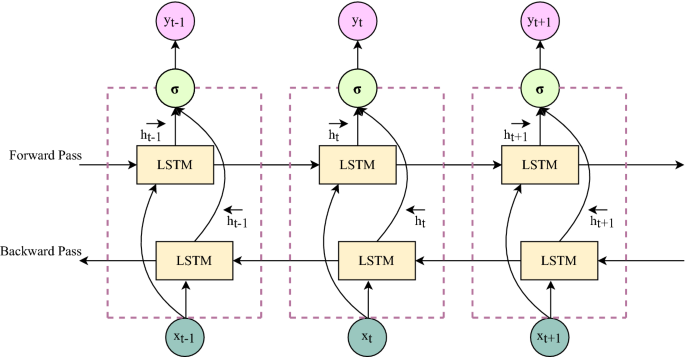
\includegraphics[width=0.5\textwidth]{LSTMs/bidirectional.png}
  \caption{Bidirectional LSTM}
  \Description{Bidirectional LSTM}
\end{figure}
\subsubsection{\textbf{Inception LSTM}}
Inception LSTMs integrate the Inception architecture with LSTM networks to create a model capable of capturing multi-scale features from sequential data. Similar to Inception modules in CNNs that utilize parallel convolutional filters of varying sizes, Inception LSTMs apply multiple LSTM layers with different configurations simultaneously. This allows the model to learn diverse temporal patterns and dependencies at various scales, making it particularly effective for complex sequence prediction tasks. The combination enhances learning efficiency and improves model performance across various applications.
\begin{figure}[h]
  \centering
  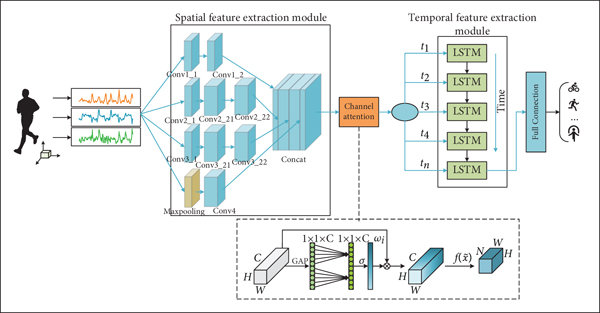
\includegraphics[width=0.5\textwidth]{LSTMs/inception.png}
  \caption{Inception LSTM}
  \Description{Inception LSTM}
\end{figure}

\subsection{Loss Function}
L1 Loss or Mean Absolute Error is used.
\[
L_1(w) = \sum_{i=1}^{n} |w_i|
\] where
\[
|w_i| = |Y_{pred}-Y_{true}|\]
Result of Loss Function for ECG5000 are given below.
\begin{figure}[ht]
    \centering

    % First row with one image
    \begin{subfigure}[b]{0.33\textwidth}
        \centering
        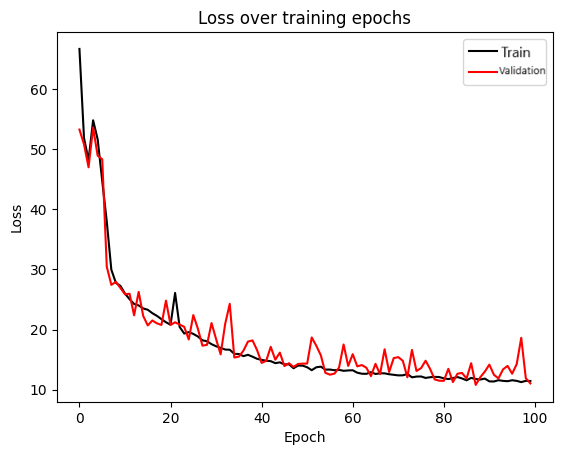
\includegraphics[width=\textwidth]{ecg5000/trainloss.png} % Replace with your image file
        \caption{Train Loss for ECG5000}
        \label{fig:first_image}
    \end{subfigure}

    % New line for the second row
    \vspace{1em} % Optional vertical space between rows

    % Second row with two images
    \begin{subfigure}[b]{0.2\textwidth}
        \centering
        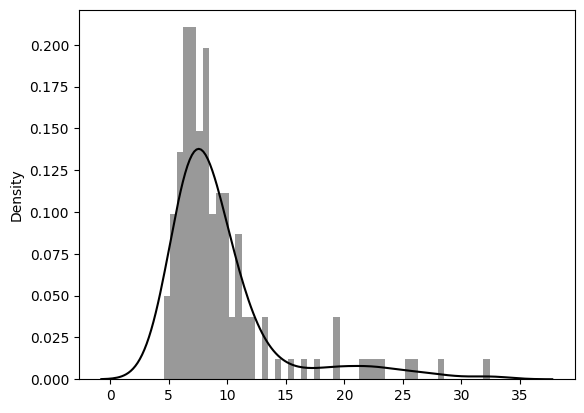
\includegraphics[width=\textwidth]{ecg5000/reconstruction_loss_normal.png} % Replace with your image file
        \caption{Reconstruction Loss for ECG5000 (Normal Data)}
        \label{fig:second_image}
    \end{subfigure}
    \hfill % This creates space between the two subfigures
    \begin{subfigure}[b]{0.2\textwidth}
        \centering
        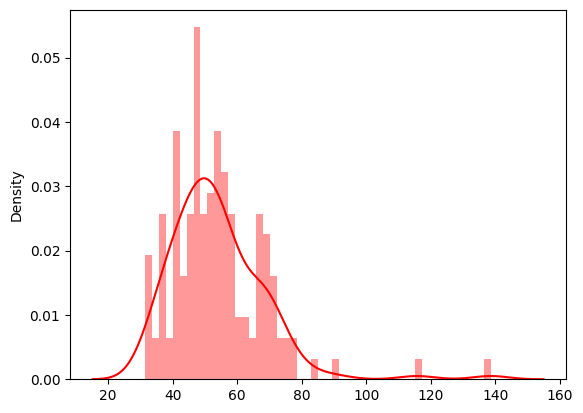
\includegraphics[width=\textwidth]{ecg5000/reconstruction_loss_abnormal.png} % Replace with your image file
        \caption{Reconstruction Loss for ECG5000 (Abnormal Data)}
        \label{fig:third_image}
    \end{subfigure}

    \caption{Loss Function Result of ECG5000}
    \label{fig:overall_figure}
\end{figure}
\\Its intuition is stated below : 
\begin{enumerate}
    \item \textbf{Robustness to Noise}: ECG signals are often contaminated with noise from various sources (e.g.,
motion artifacts, electrical interference). L1 loss, by measuring absolute differences, is less sensitive
to outliers and noise compared to L2 loss.
\item \textbf{ Simplicity in Interpretation}: The absolute error calculated by L1 loss provides a straightforward
interpretation of how far predictions deviate from actual classifications.
\item \textbf{ Temporal Context Preservation}: LSTM networks are designed to capture temporal dependencies
in sequential data like ECG signals. When combined with L1 loss, the model can effectively learn to
identify patterns over time while maintaining robustness against abrupt changes or noise within
individual heartbeats.
\item \textbf{ Facilitating Model Training}: The optimization landscape created by L1 loss tends to be simpler
than that of squared losses, potentially leading to faster convergence during training.  

\end{enumerate}


\subsection{Performance Metrics}
\begin{enumerate}
    \item \textbf{Threshold for Anomalies}: A predefined value set to distinguish between normal and anomalous readings based on reconstruction loss. Data points with reconstruction loss exceeding this threshold are classified as anomalies.

\item \textbf{Accuracy}: A metric that measures the proportion of true results (both true positives and true negatives) among the total number of cases examined. It is calculated as:
$$
\text{Accuracy} = \frac{TP + TN}{TP + TN + FP + FN}
$$

\item \textbf{Precision}: Also known as positive predictive value, it quantifies the number of true positive results divided by the sum of true positives and false positives. It is expressed as:
$$
\text{Precision} = \frac{TP}{TP + FP}
$$

\item \textbf{Recall or Sensitivity}: Also referred to as sensitivity or true positive rate, it measures the ability of a model to find all relevant cases (true positives) in a dataset. It is calculated as:
$$
\text{Recall} = \frac{TP}{TP + FN}
$$

\item \textbf{F1-Score}: The harmonic mean of precision and recall, providing a balance between the two metrics. It is especially useful when dealing with imbalanced datasets. The formula is:
$$
F1 = 2 \cdot \frac{\text{Precision} \cdot \text{Recall}}{\text{Precision} + \text{Recall}}
$$
\item \textbf{AUROC (Area Under the Receiver Operating Characteristic Curve)}: A performance measurement for classification problems at various threshold settings. AUROC represents the degree or measure of separability achieved by a model, indicating how well it can distinguish between positive and negative classes. It ranges from 0 to 1, where 1 indicates perfect classification and 0.5 indicates no discriminative power.
\item \textbf{Plot Prediction}: A function that visualizes both the original and reconstructed sequences (e.g., ECG signals) alongside their respective reconstruction losses. This helps in assessing model performance at an individual sequence level, allowing for better understanding of how well the model reconstructs normal versus anomalous data.

\end{enumerate}

\subsection{SHAP Analysis}
In this analysis, we employed SHAP (SHapley Additive exPlanations) to interpret the predictions made by our machine learning models on the ECG5000 dataset.
\subsubsection{\textbf{Purpose of SHAP Analysis}}
The primary objective of using SHAP was to gain insights into the contributions of individual features to the model's predictions. By understanding which features are most influential, we can enhance model transparency, improve interpretability, and identify potential areas for further investigation in the context of ECG analysis.
\subsubsection{\textbf{
Methodology}}
\begin{enumerate} 
    \item \textbf{Model Training}: We trained a suitable machine learning model (e.g.Gradient Explainer) on the ECG5000 dataset.
    \item \textbf{SHAP Value Calculation}: We utilized the SHAP library to compute SHAP values for each feature in the dataset. These values indicate how much each feature contributes to the difference between the model's prediction and the average prediction across all samples.
    \item \textbf{Visualization}: We created visualizations such as summary plots and dependence plots to illustrate the impact of features on model predictions.
\end{enumerate}
\subsubsection{\textbf{Key Findings}}

\begin{enumerate}
    \item \textbf{
    Feature Importance}: The analysis revealed that certain features significantly influenced the model's predictions, allowing us to identify key characteristics associated with different ECG patterns.
    
    \item \textbf{Insights into Model Behavior}: By examining SHAP values, we could understand how specific changes in feature values affected predictions, providing a clearer picture of model behavior.
    
\end{enumerate}
\subsubsection{\textbf{Challenges}}
Due to gpu memory insufficiency, we cannot do SHAP analysis on big dataset and large models. Besides, we have some time constraints, so small dataset is used for SHAP analysis.Dataset used for SHAP consists of 500 normal data and500 abnormal data.This samll dataset is used to fit the model as well as SHAP analysis.

\subsection{Implementation}
Codes are available \href{https://github.com/1905046-NiazRahman/CSE472-Project}{\textcolor{blue}{here}}.


\subsection{Training and Test Set Details}
\subsubsection{\textbf{ECG5000}}
We have used the full dataset for train and testing our model.There are total 5000 data. We have split the dataset like this:
\begin{itemize}
    \item Training Dataset: 500 normal data entries
    \item Validation Dataset: 500 normal data entries
    \item Test Dataset: 4000 data entries(both normal and abnormal)
\end{itemize}
\subsubsection{\textbf{MIT-BIH}}
In our analysis, we initially generated a very large dataset consisting of 112,580 data entries, each containing 140 data points using interpolation. Due to resource and time constraints, we selected a smaller, random subset for our study. This subset includes:
\begin{itemize}
    \item Training Dataset: 1,000 normal data entries
    \item Validation Dataset: 250 normal data entries
    \item Test Dataset: 250 normal data entries and 250 abnormal data entries
\end{itemize}
This strategic selection allows us to effectively manage our resources while still ensuring robust model evaluation.

\section{Result and Discussion}
\subsection{ECG5000}

\subsubsection{\textbf{Performance Metrics}}
We have compare the accuracy, precision, recall, f1-score and auroc among our models, base paper model and state of the art method models.The result is shown in the table \ref{Tab:ECG5000_Table} and the bar diagram is shown in the figure \ref{tab:Fig1}.
\begin{table}[h]
\caption{Comparison of Performance Metrics of ECG5000}
  \label{Tab:ECG5000_Table}
  \resizebox{0.5\textwidth}{!}{
\begin{tabular}{|r|r|r|r|r|r|}
\hline
\multicolumn{1}{|l|}{{\color[HTML]{000000} Model Name}}     & {\color[HTML]{000000} \textbf{precision}} & {\color[HTML]{000000} \textbf{recall}} & {\color[HTML]{000000} \textbf{f1}} & {\color[HTML]{000000} \textbf{accuracy}} & {\color[HTML]{000000} \textbf{AUROC}} \\ \hline
{\color[HTML]{000000} LSTM }                     & {\color[HTML]{000000} 0.96}                      & {\color[HTML]{000000} 0.96}                   & {\color[HTML]{000000} 0.95}               & {\color[HTML]{000000} 0.95}                     & {\color[HTML]{000000} 0.96}           \\ \hline
{\color[HTML]{000000} Stacked LSTM }             & {\color[HTML]{000000} 0.97}                      & {\color[HTML]{000000} 0.97}                   & {\color[HTML]{000000} 0.97}               & {\color[HTML]{000000} 0.98}                     & {\color[HTML]{000000} 0.97}           \\ \hline
{\color[HTML]{000000} CNN LSTM }                 & {\color[HTML]{000000} 0.98}                      & {\color[HTML]{000000} 0.97}                   & {\color[HTML]{000000} 0.98}               & {\color[HTML]{000000} 0.98}                     & {\color[HTML]{000000} 0.97}           \\ \hline
{\color[HTML]{000000} Bidirectional LSTM }       & {\color[HTML]{000000} 0.94}                      & {\color[HTML]{000000} 0.96}                   & {\color[HTML]{000000} 0.95}               & {\color[HTML]{000000} 0.95}                     & {\color[HTML]{000000} 0.95}           \\ \hline
{\color[HTML]{000000} Inception LSTM }           & {\color[HTML]{000000} 0.98}                      & {\color[HTML]{000000} 0.97}                   & {\color[HTML]{000000} 0.98}               & {\color[HTML]{000000} 0.97}                     & {\color[HTML]{000000} 0.98}           \\ \hline
{\color[HTML]{000000} ECG-Net}                 & {\color[HTML]{000000} 0.95}                      & {\color[HTML]{000000} 0.97}                   & {\color[HTML]{000000} 0.98}               & {\color[HTML]{000000} 0.98}                     & {\color[HTML]{000000} 0.98}           \\ \hline
{\color[HTML]{000000} Transformer} & {\color[HTML]{000000} 1.00}                      & {\color[HTML]{000000} 0.98}                   & {\color[HTML]{000000} 0.99}               & {\color[HTML]{000000} 0.99}                     & {\color[HTML]{000000} 0.98}           \\ \hline
\end{tabular}}
\end{table}
\begin{figure}[h]
  \centering
  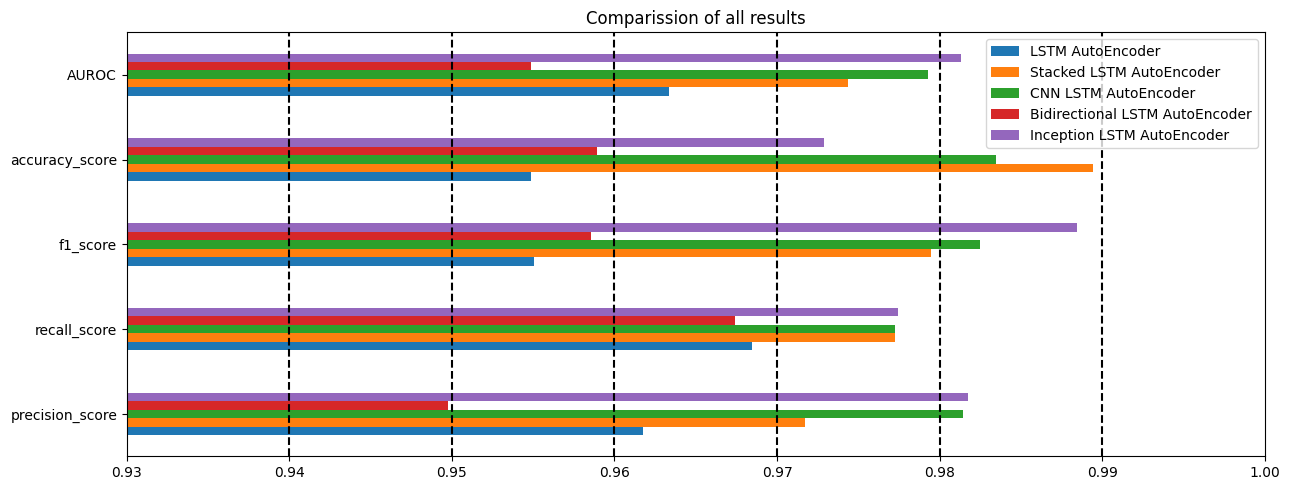
\includegraphics[width=0.5\textwidth]{ecg5000/performance.png}
  \caption{Comparison of Performance Metrics of ECG5000}
  \Description{Comparison of Performance Metrics of ECG5000}
  \label{tab:Fig1}
\end{figure}


\subsubsection{\textbf{Plot Prediction Insights}}
\begin{enumerate}
    \item \textbf{True Positive}:All the models reproduced the normal heartbeat sequences very well.Inception LSTM has small reconstruction loss. On the other hand, Bidirectional LSTM has large reconstruction loss that means it triew to predict correct data as anomaly.
    \item \textbf{True Negative}
    The CNN and Inception LSTM AutoEncoder learned the same pattern as LSTM AutoEncoders and also remembered a significant drop at the beginning of the sequence.In contrast, The Bidirectional LSTM AutoEncoder isn't good solution for this problem. It looks like the model learned that in normal heartbeats occur a significant drops and extra small peaks at the beginning and at the end of sequence.

    \item \textbf{False Positive}
    Bidirectional LSTM AutoEncoders have classified many normal sequences as anomalies. The lower loss in false positive examples proves that these models are slightly overfitted.Besides, LSTM, Stacked LSTM and CNN LStm AutoEncoders made only 4 false positive errors. Interestingly, these models were mistaken on the same samples.

    \item \textbf{False Negative}
    LSTM and Bidirectional LSTM AutoEncoders have classified the most normal sequences as anomalies.Interestingly, all models were mistaken on almost the same samples    
\end{enumerate}
    \begin{figure}
        \centering
        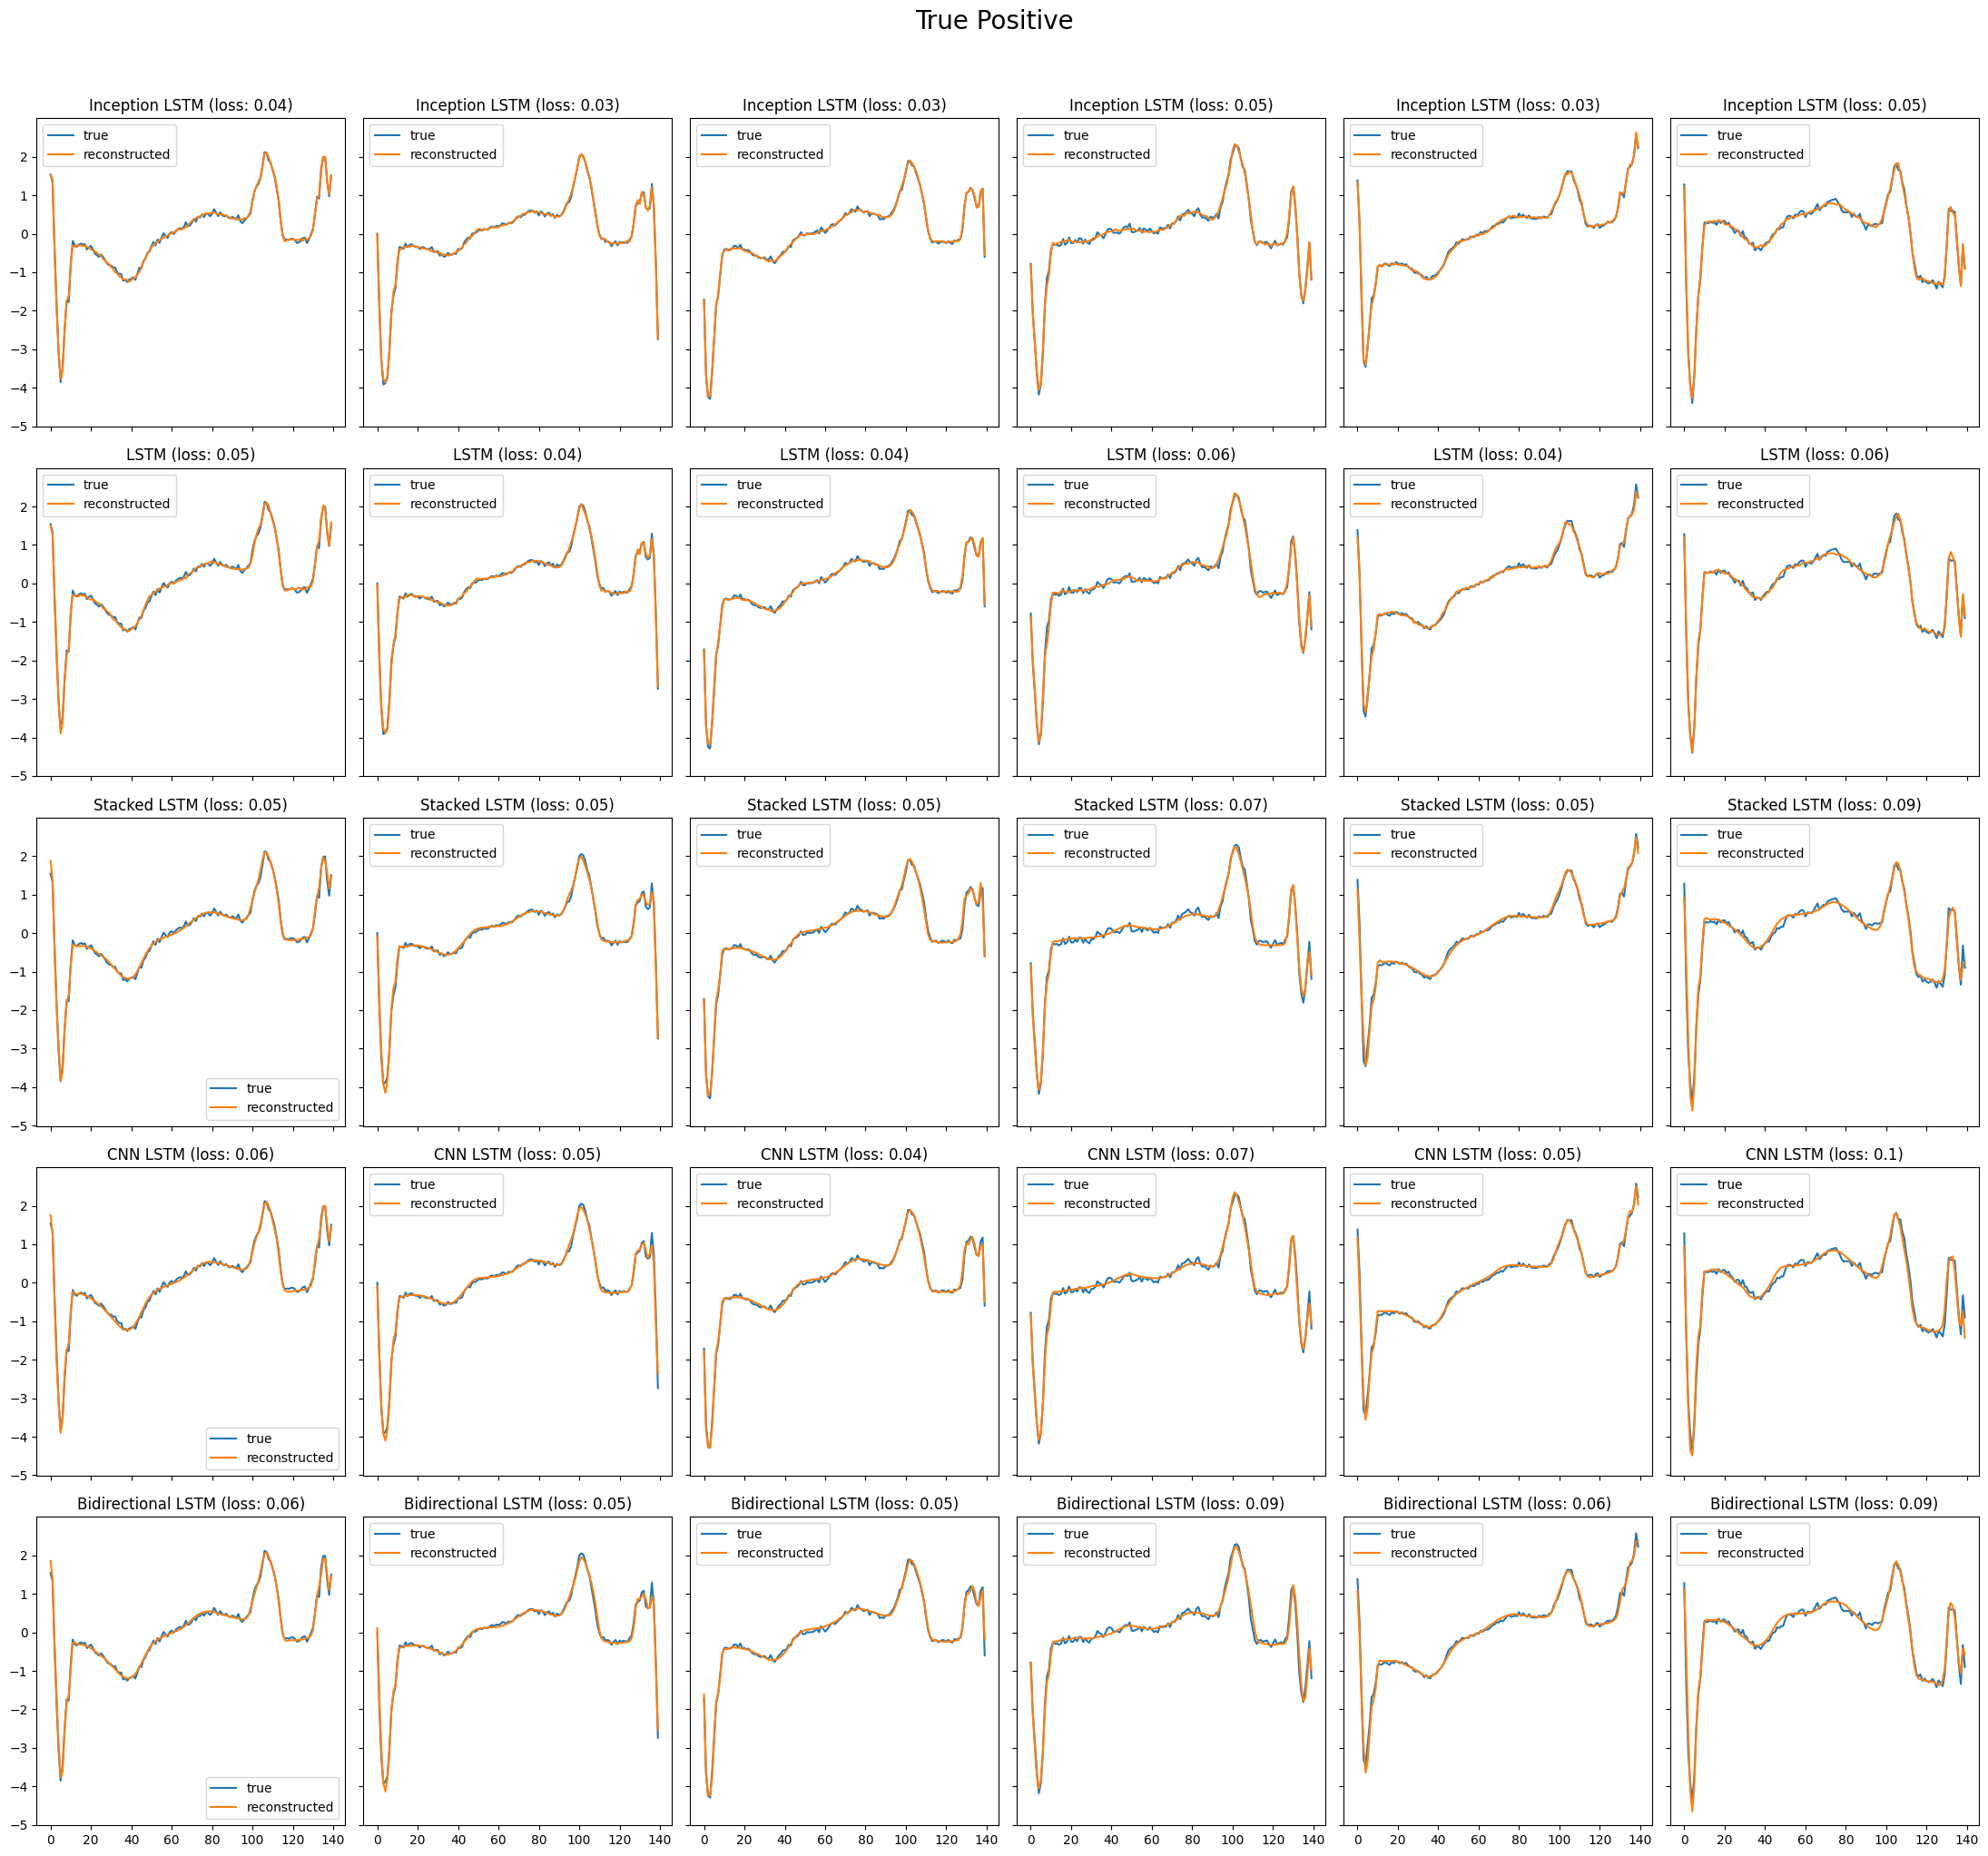
\includegraphics[width=0.35\textwidth]{ecg5000/TP.png}
        \caption{Compare true positive reconstructed sequences of ecg5000 (normal heartbeats sequences classified as normal)}
        \label{fig:image1}
    \end{figure}%
        \begin{figure}
        \centering
        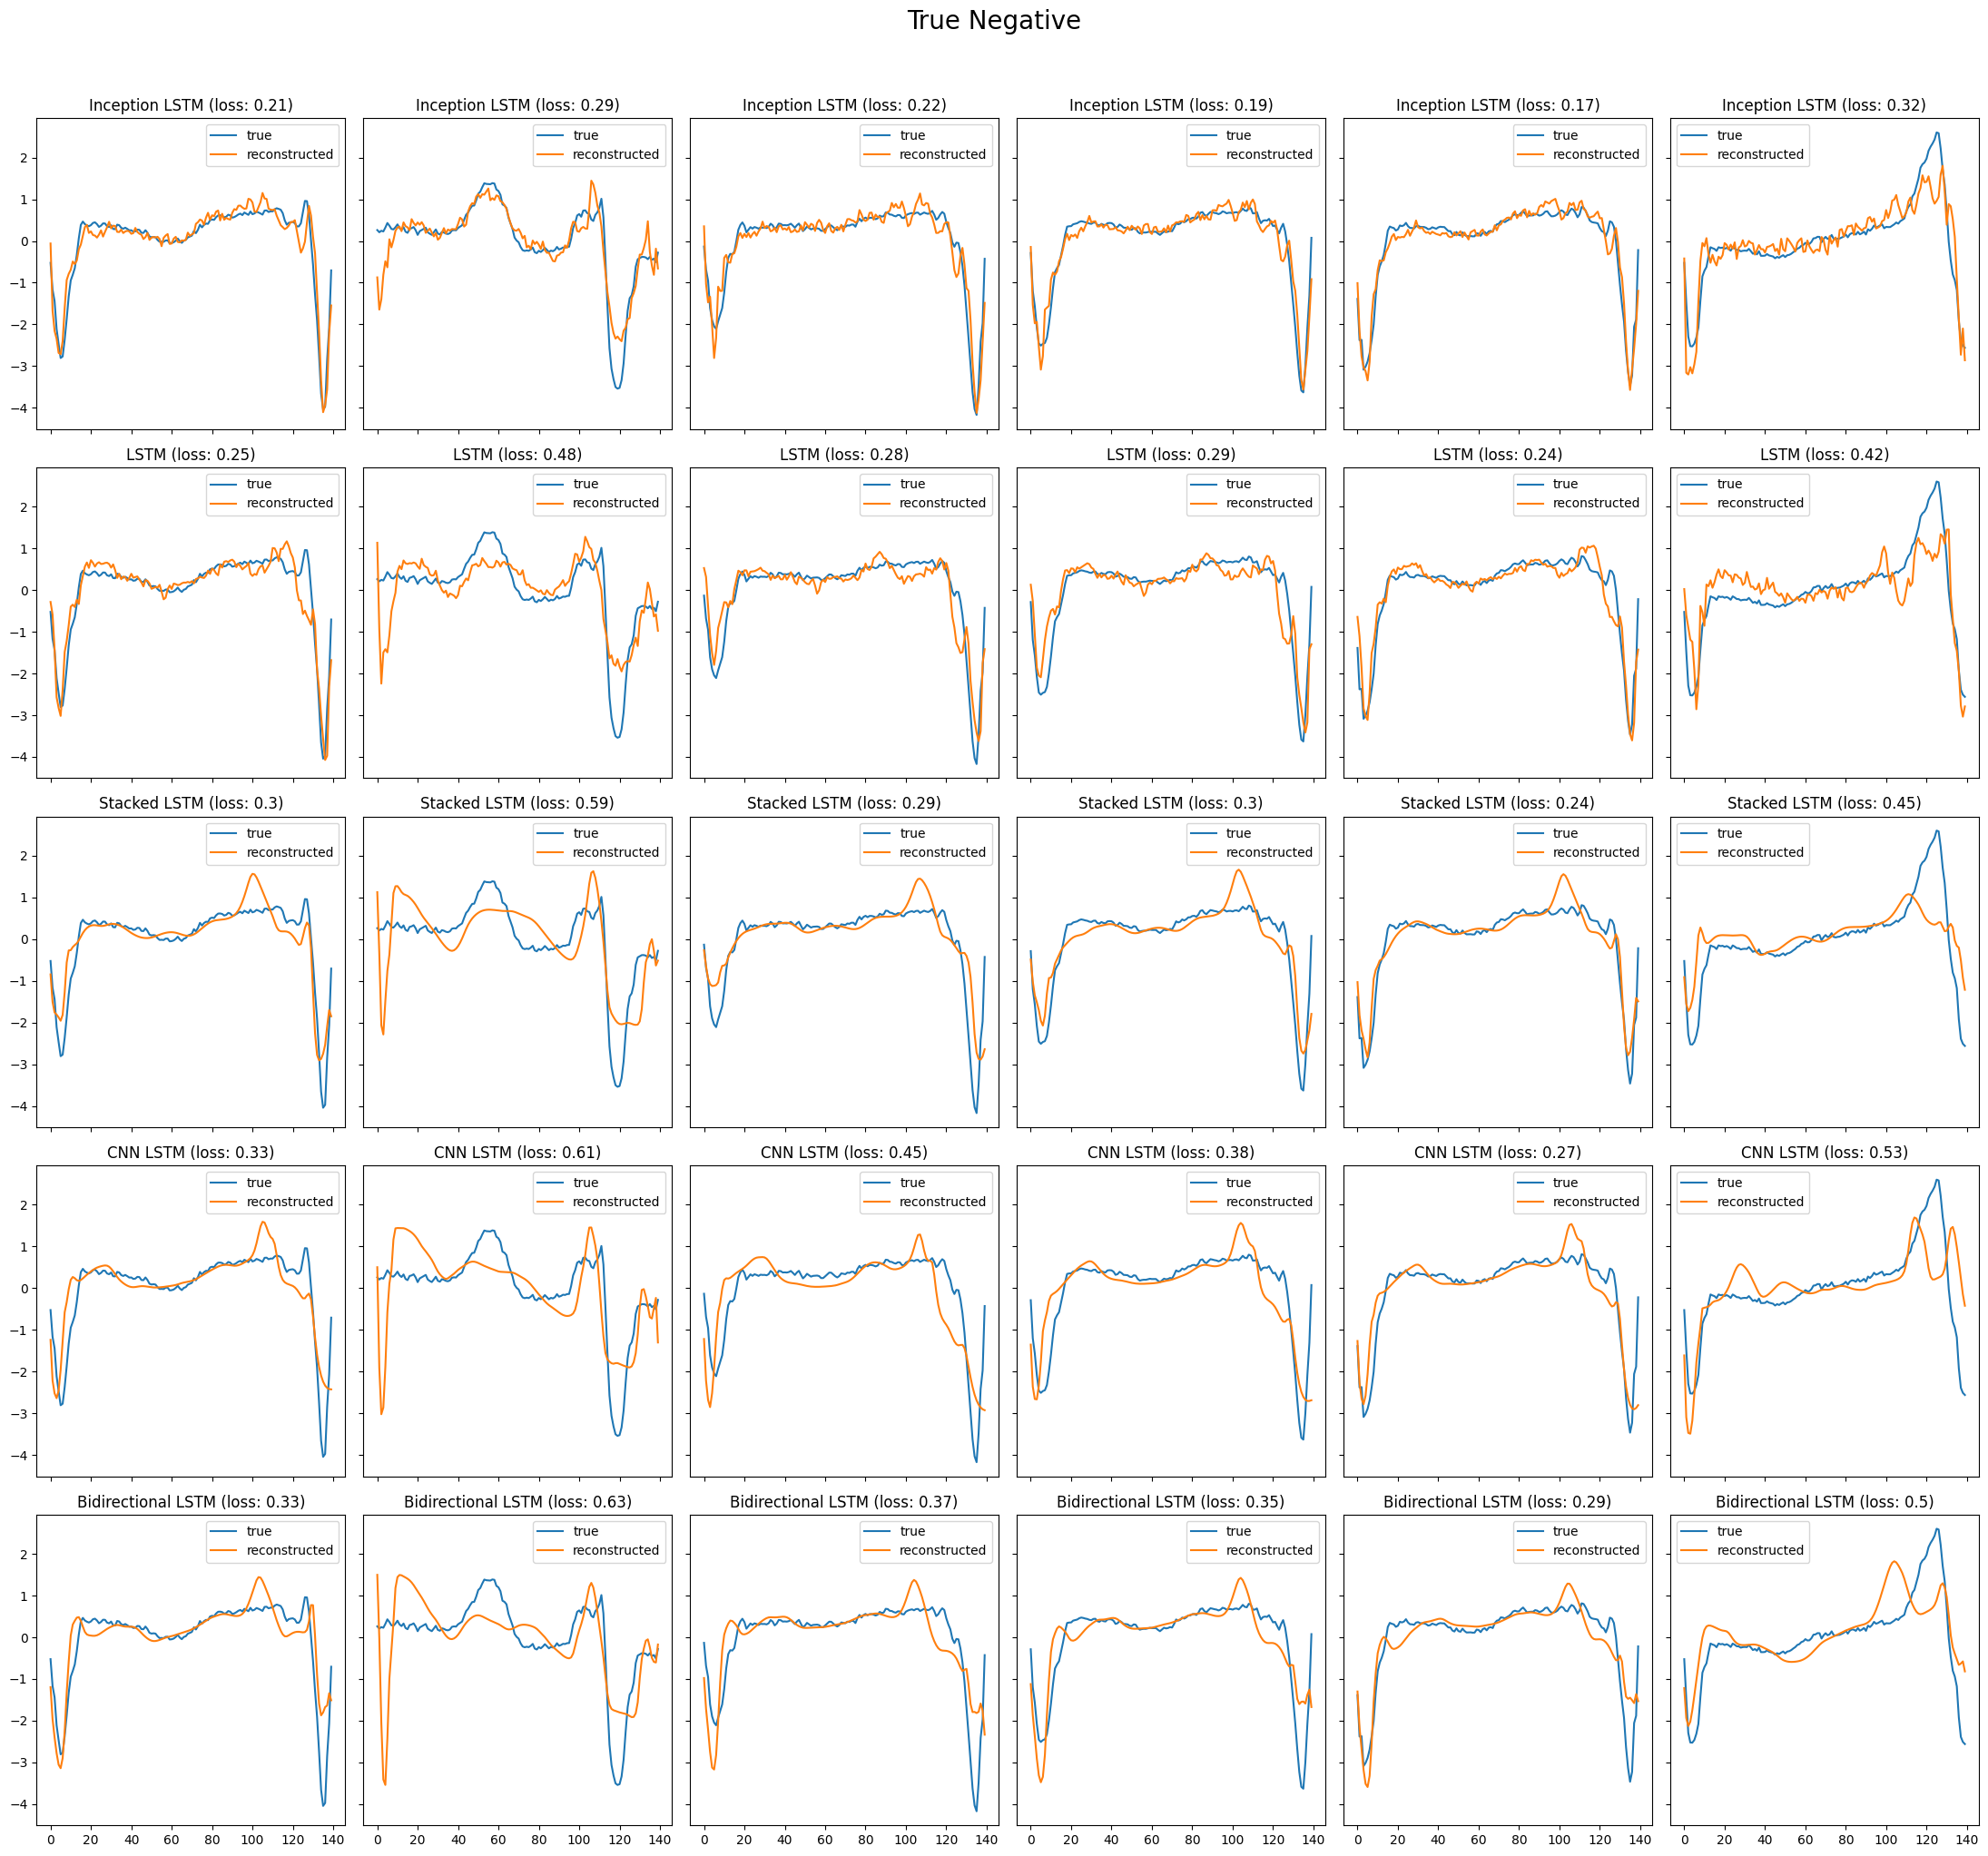
\includegraphics[width=0.35\textwidth]{ecg5000/TN.png}
        \caption{Compare true negative reconstructed sequences of ecg5000 (anomaly heartbeats sequences classified as anomaly)}
        \label{fig:image1}
    \end{figure}%
        \begin{figure}
        \centering
        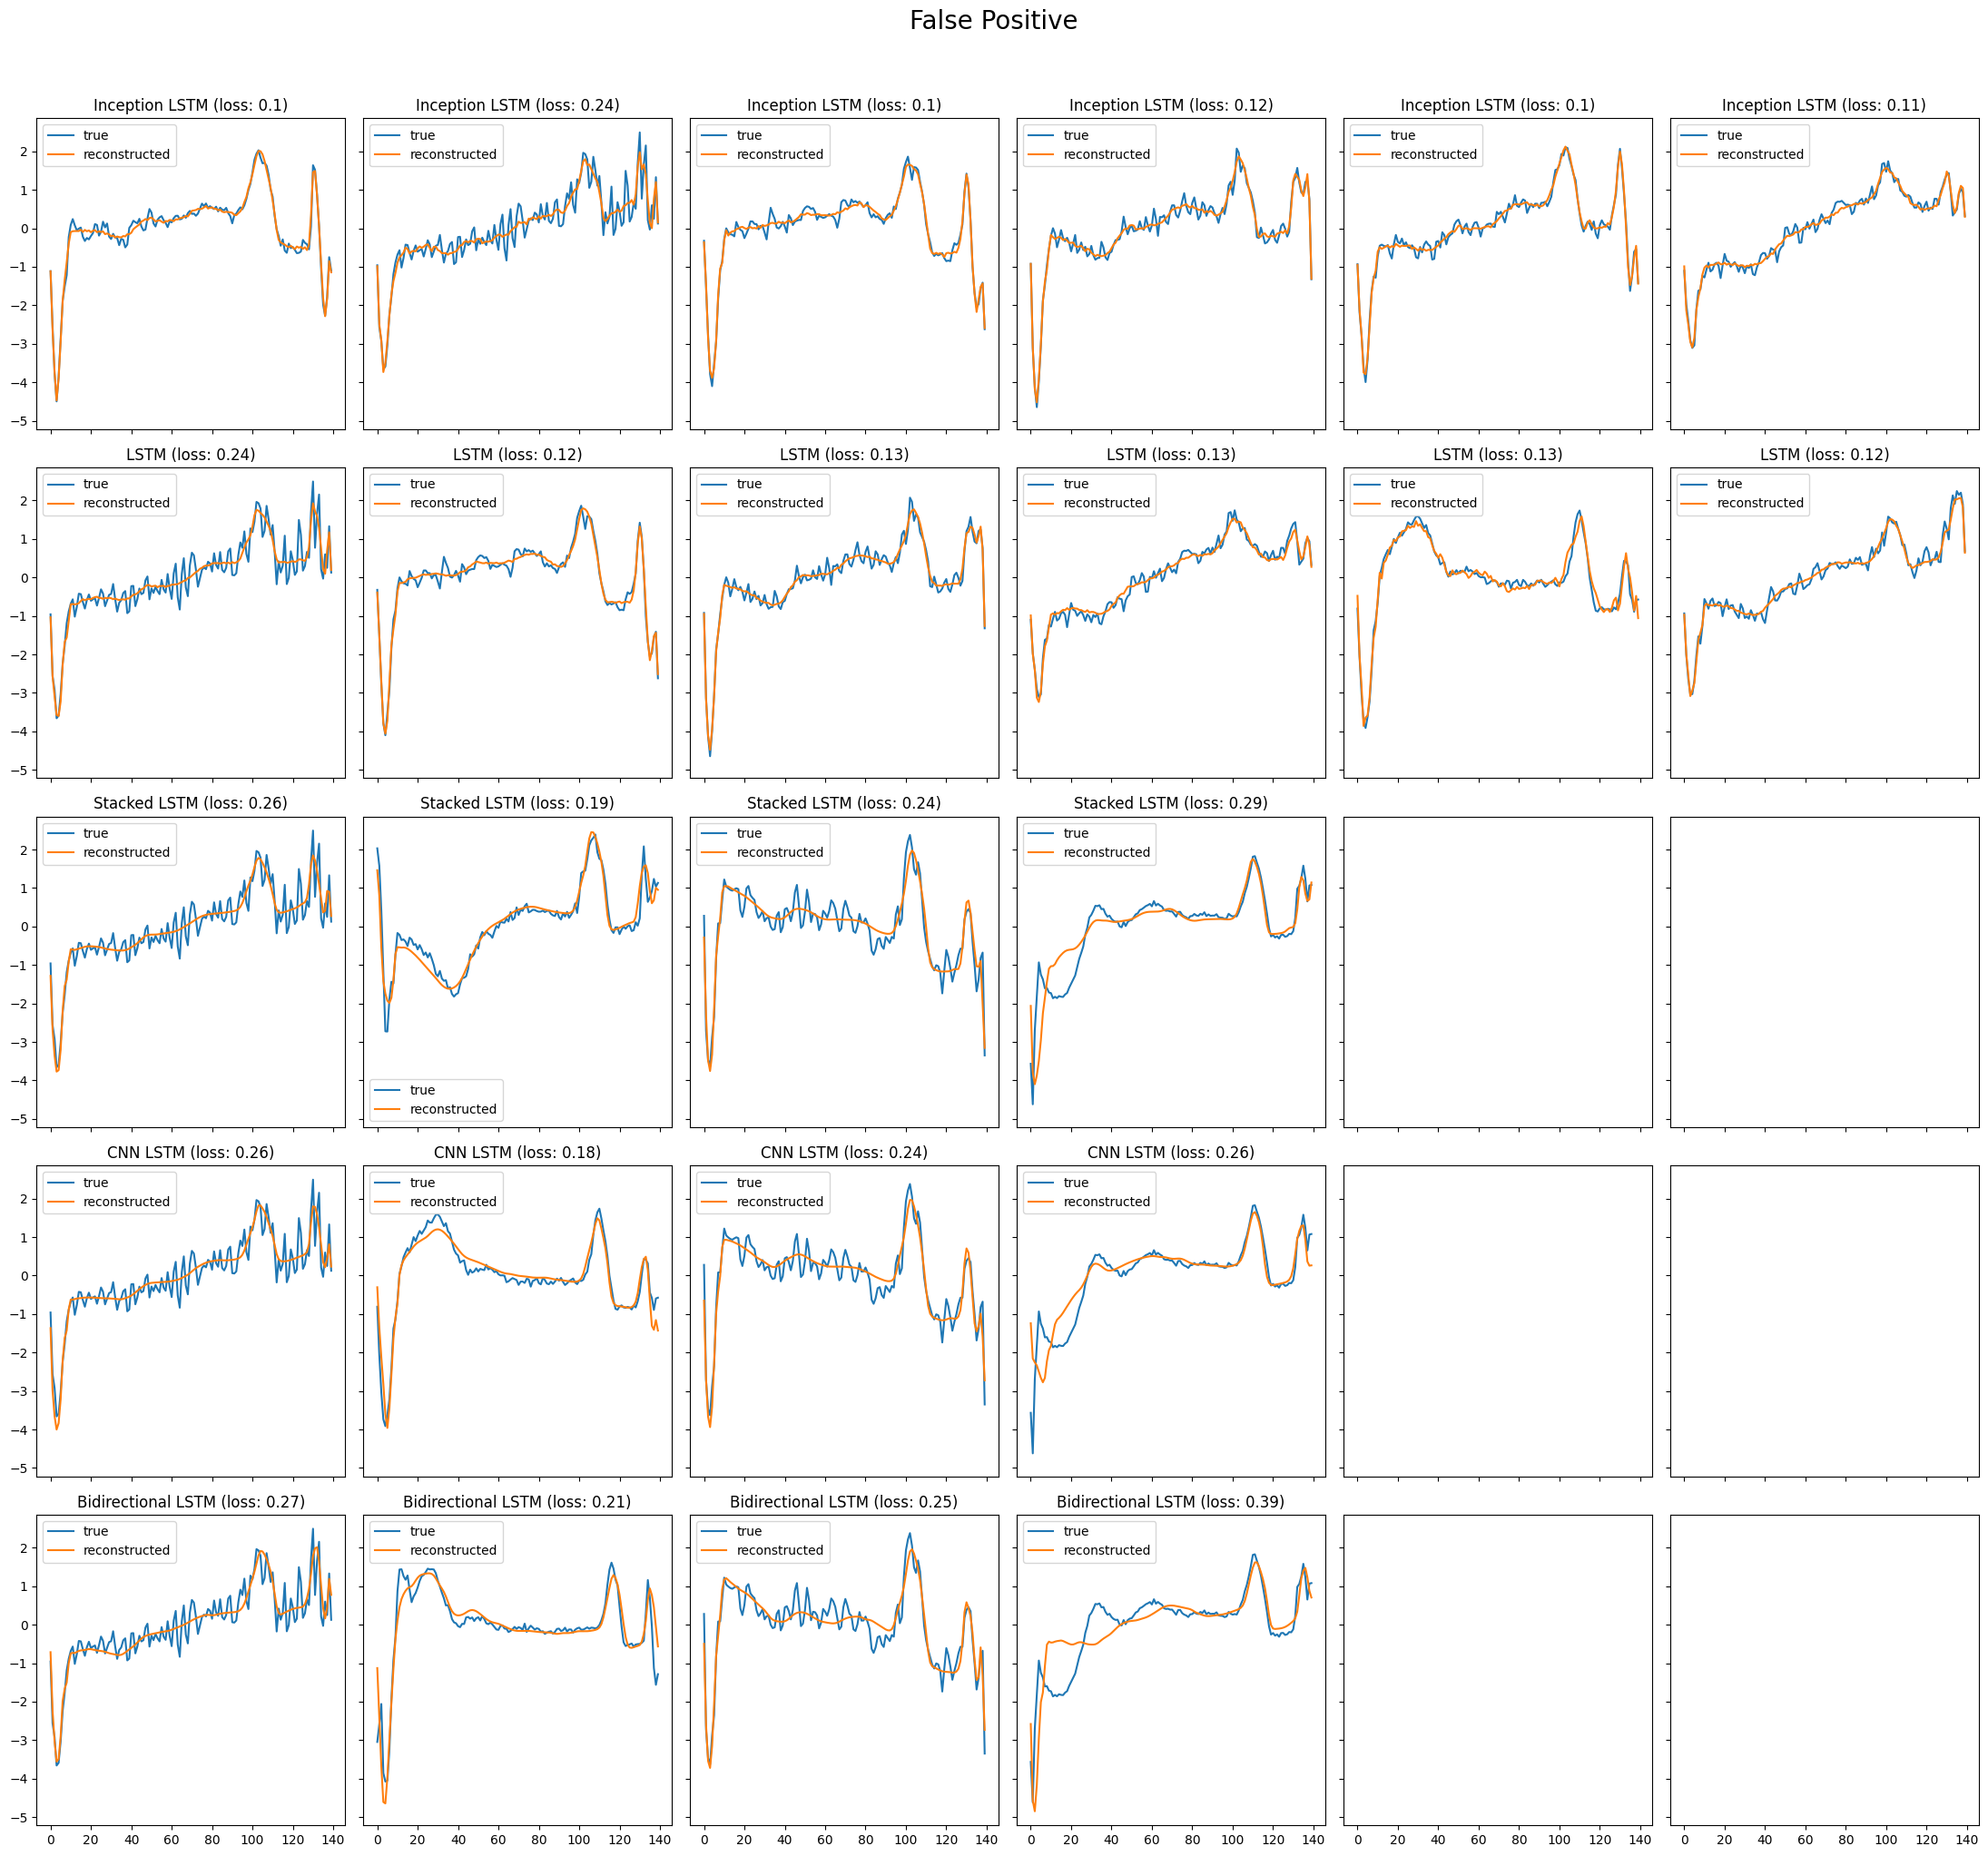
\includegraphics[width=0.35\textwidth]{ecg5000/FP.png}
        \caption{Compare false positive reconstructed sequences of ecg5000 (anomaly heartbeats sequences classified as normal)}
        \label{fig:image1}
    \end{figure}%
        \begin{figure}
        \centering
        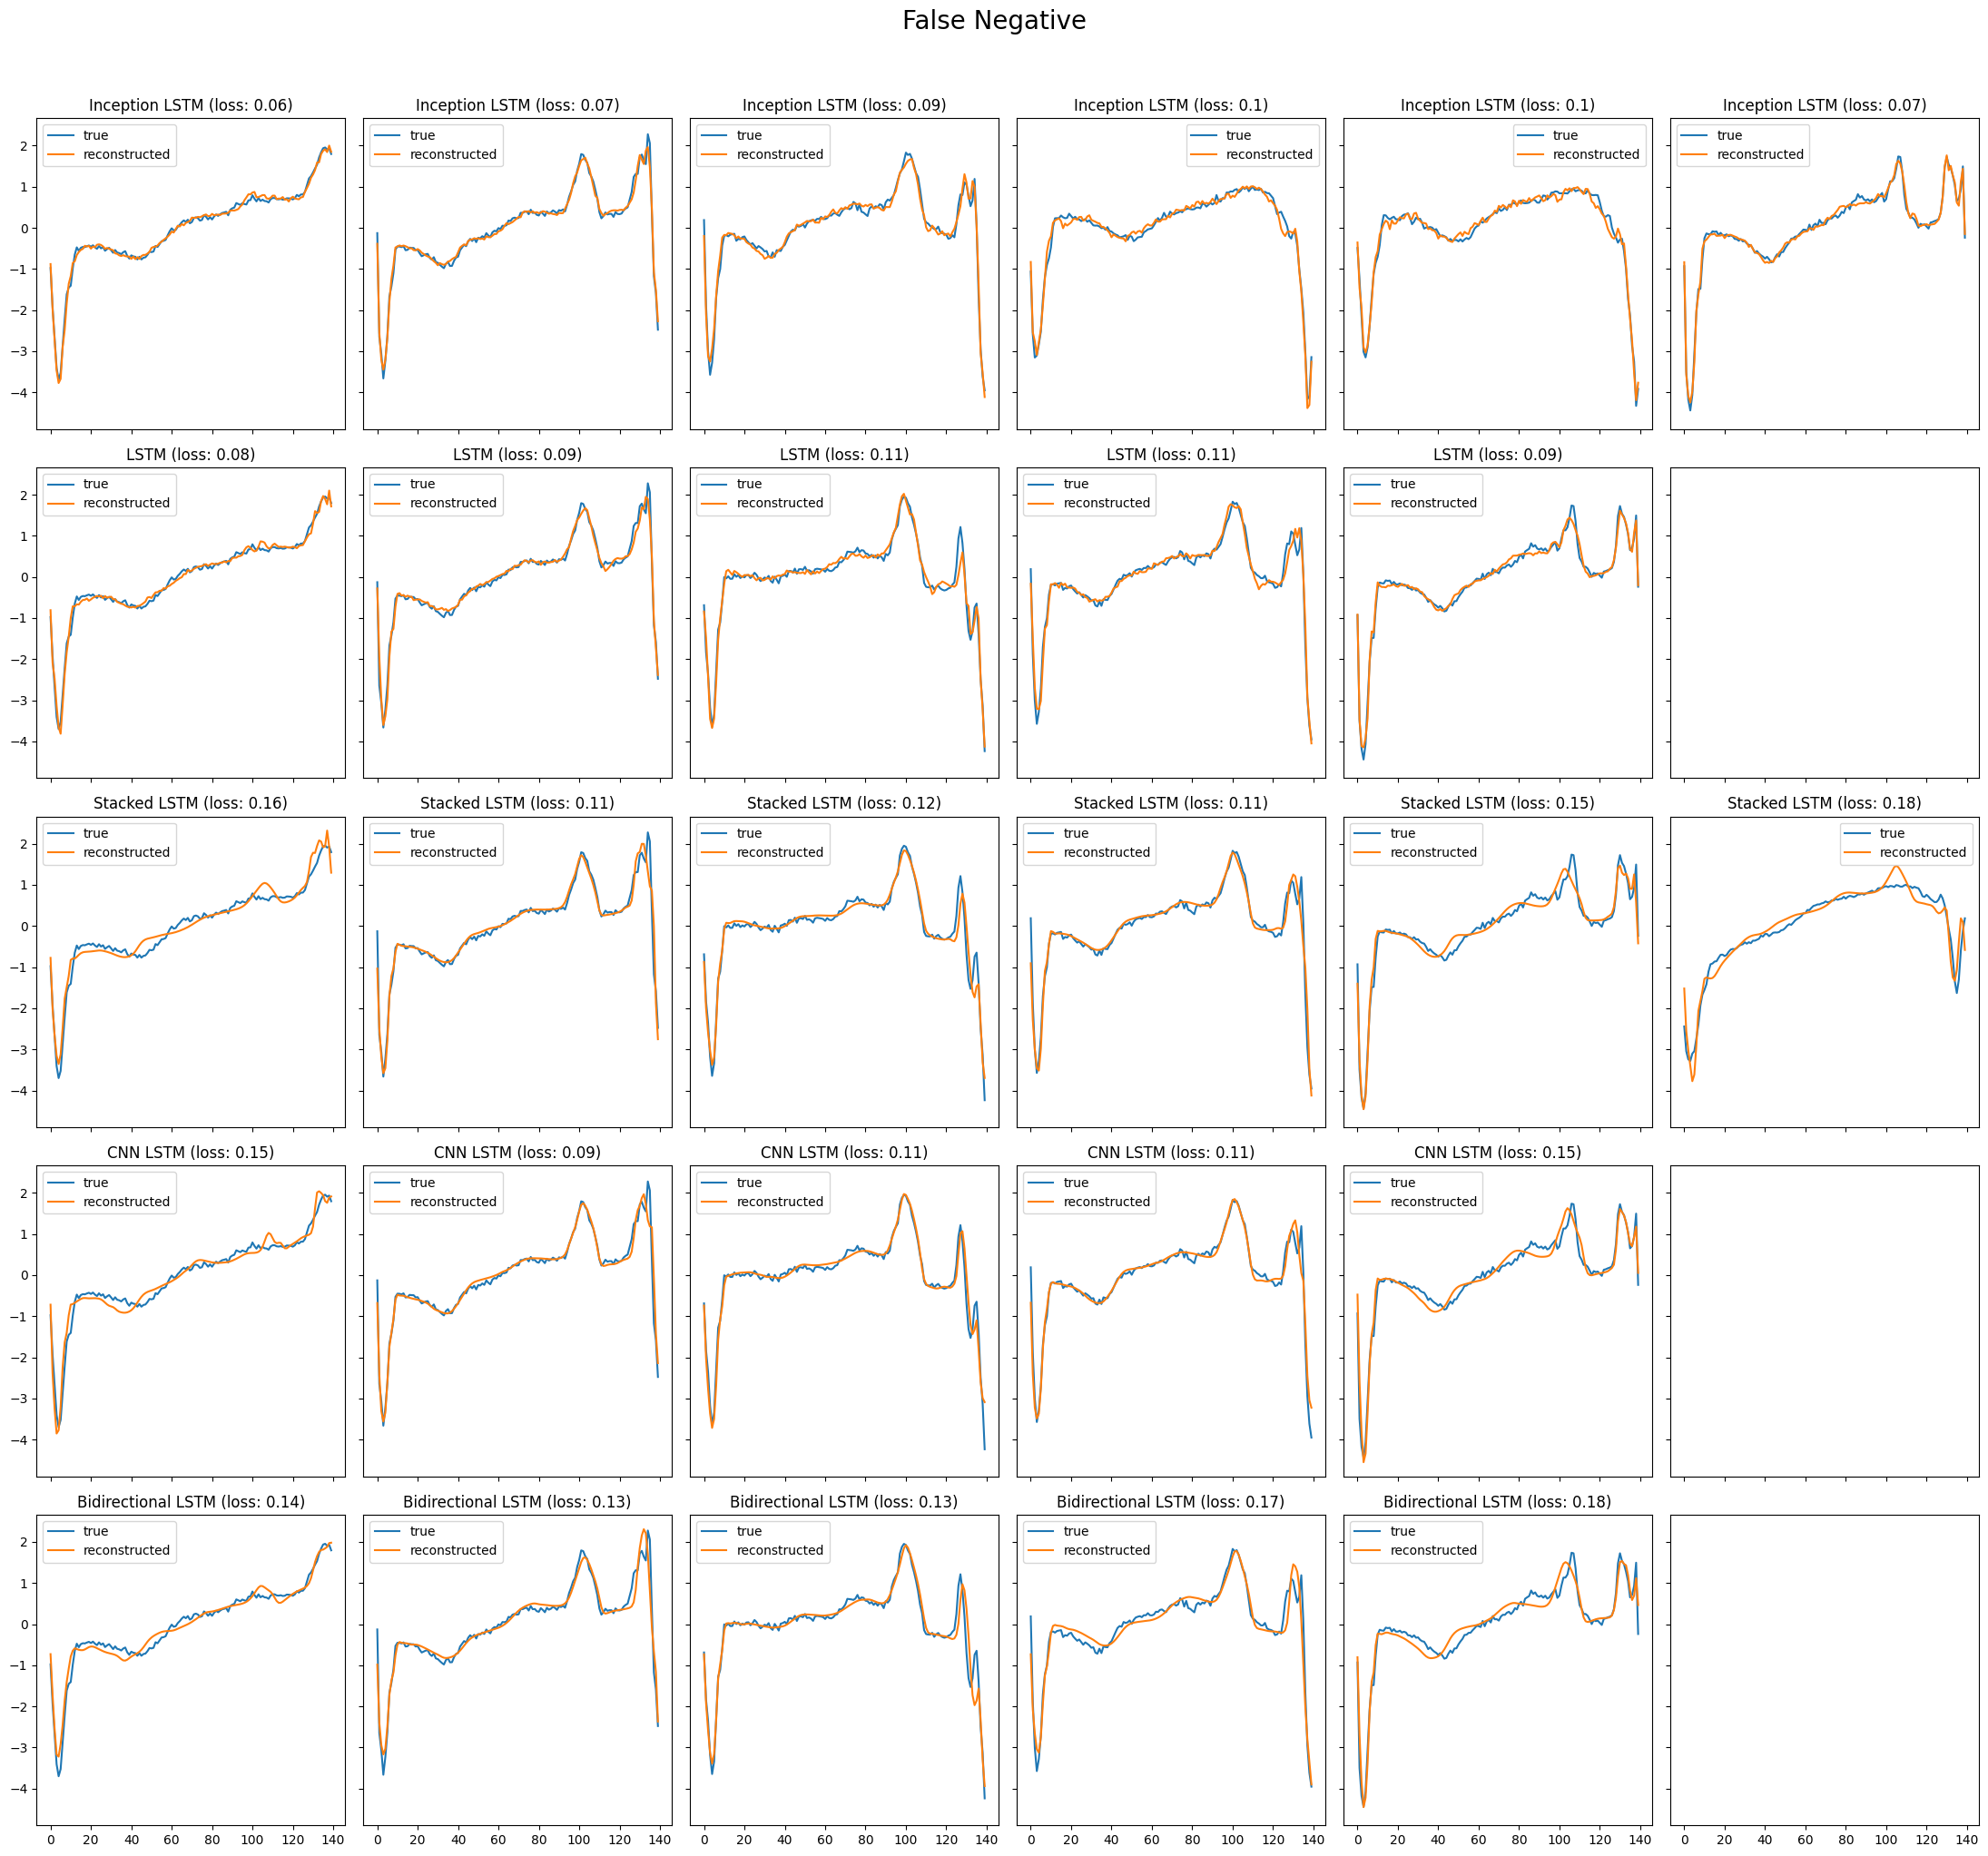
\includegraphics[width=0.35\textwidth]{ecg5000/FN.png}
        \caption{Compare false negative reconstructed sequences of ecg5000 (normal heartbeats sequences classified as anomaly)}
        \label{fig:image1}
    \end{figure}%
Plot prediction in machine learning refers to the visual representation of model predictions compared to actual outcomes. This practice is crucial for evaluating and diagnosing the performance of regression models.
\subsection{MIT-BIH}
\subsubsection{\textbf{Performance Metrics}}
We have compare the accuracy, precision, recall, f1-score and auroc among our models, base paper model and state of the art method models.The result is shown in the table \ref{Tab:MIT_BIH_table} and the bar diagram is shown in the figure \ref{tab:Fig2}

Though our models achieve good precision score but they have done bad perdormance in other metrics.
\begin{table}[h]
\caption{Comparison of Performance Metrics of MIT-BIH}
\label{Tab:MIT_BIH_table}
\resizebox{0.5\textwidth}{!}{
\begin{tabular}{|r|r|r|r|r|r|}
\hline
{\color[HTML]{333333} \textbf{Model Name}}                     & {\color[HTML]{333333} \textbf{precision}} & {\color[HTML]{333333} \textbf{recall}} & {\color[HTML]{333333} \textbf{f1}} & {\color[HTML]{333333} \textbf{accuracy}} & {\color[HTML]{333333} \textbf{AUROC}} \\ \hline
{\color[HTML]{333333} \textbf{LSTM}}               & {\color[HTML]{333333} \textbf{0.992}}            & {\color[HTML]{333333} \textbf{0.508}}         & {\color[HTML]{333333} \textbf{0.672}}     & {\color[HTML]{333333} \textbf{0.516}}           & {\color[HTML]{333333} \textbf{0.516}} \\ \hline
{\color[HTML]{333333} \textbf{Stacked LSTM}}       & {\color[HTML]{333333} \textbf{0.984}}            & {\color[HTML]{333333} \textbf{0.506}}         & {\color[HTML]{333333} \textbf{0.668}}     & {\color[HTML]{333333} \textbf{0.512}}           & {\color[HTML]{333333} \textbf{0.512}} \\ \hline
{\color[HTML]{333333} \textbf{CNN LSTM}}           & {\color[HTML]{333333} \textbf{0.984}}            & {\color[HTML]{333333} \textbf{0.506}}         & {\color[HTML]{333333} \textbf{0.668}}     & {\color[HTML]{333333} \textbf{0.512}}           & {\color[HTML]{333333} \textbf{0.512}} \\ \hline
{\color[HTML]{333333} \textbf{Bidirectional LSTM}} & {\color[HTML]{333333} \textbf{0.984}}            & {\color[HTML]{333333} \textbf{0.506}}         & {\color[HTML]{333333} \textbf{0.668}}     & {\color[HTML]{333333} \textbf{0.512}}           & {\color[HTML]{333333} \textbf{0.512}} \\ \hline
{\color[HTML]{333333} \textbf{Inception LSTM}} & {\color[HTML]{333333} \textbf{0.984}}            & {\color[HTML]{333333} \textbf{0.504}}         & {\color[HTML]{333333} \textbf{0.666}}     & {\color[HTML]{333333} \textbf{0.508}}           & {\color[HTML]{333333} \textbf{0.508}} \\ \hline
\end{tabular}
}
\end{table}
\begin{figure}[h]
  \centering
  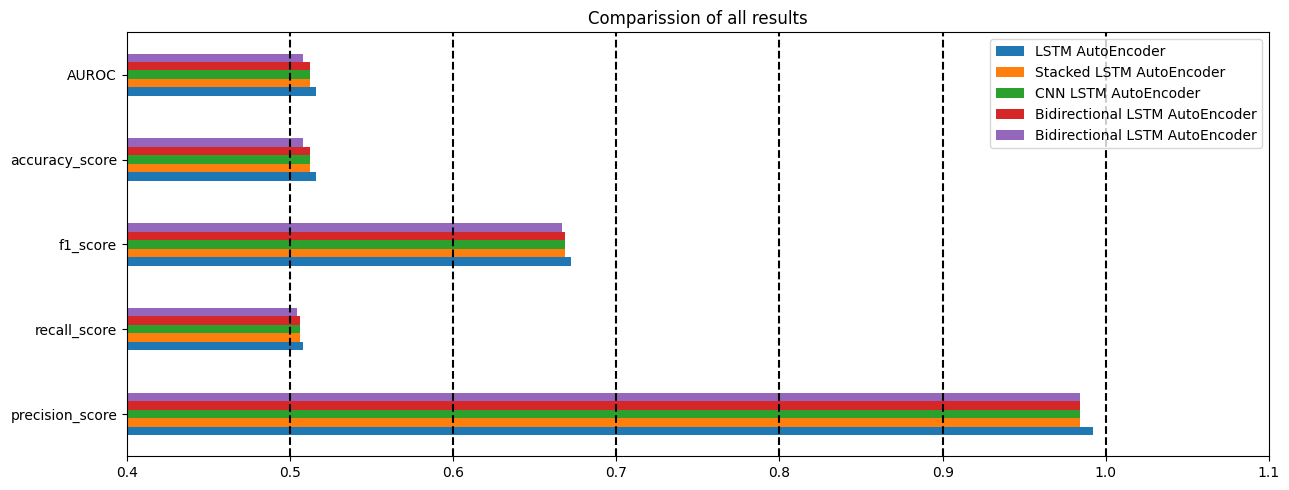
\includegraphics[width=0.5\textwidth]{MIT-BIH/performance.png}
  \caption{Comparison of Performance Metrics of MIT-BIH}
  \Description{Comparison of Performance Metrics of MIT-BIH}
  \label{tab:Fig2}
\end{figure}



\subsubsection{\textbf{Plot Prediction}}
We cannot make any decision because reconstructed sequence is plotted very bad.We have already mention the possible causes in the previous 
section.Interestingly,A useful insights we get is almost all model predicted many normal sequences as anomalies. But they predicted few anomalies as normal sequences.
    \begin{figure}
        \centering
        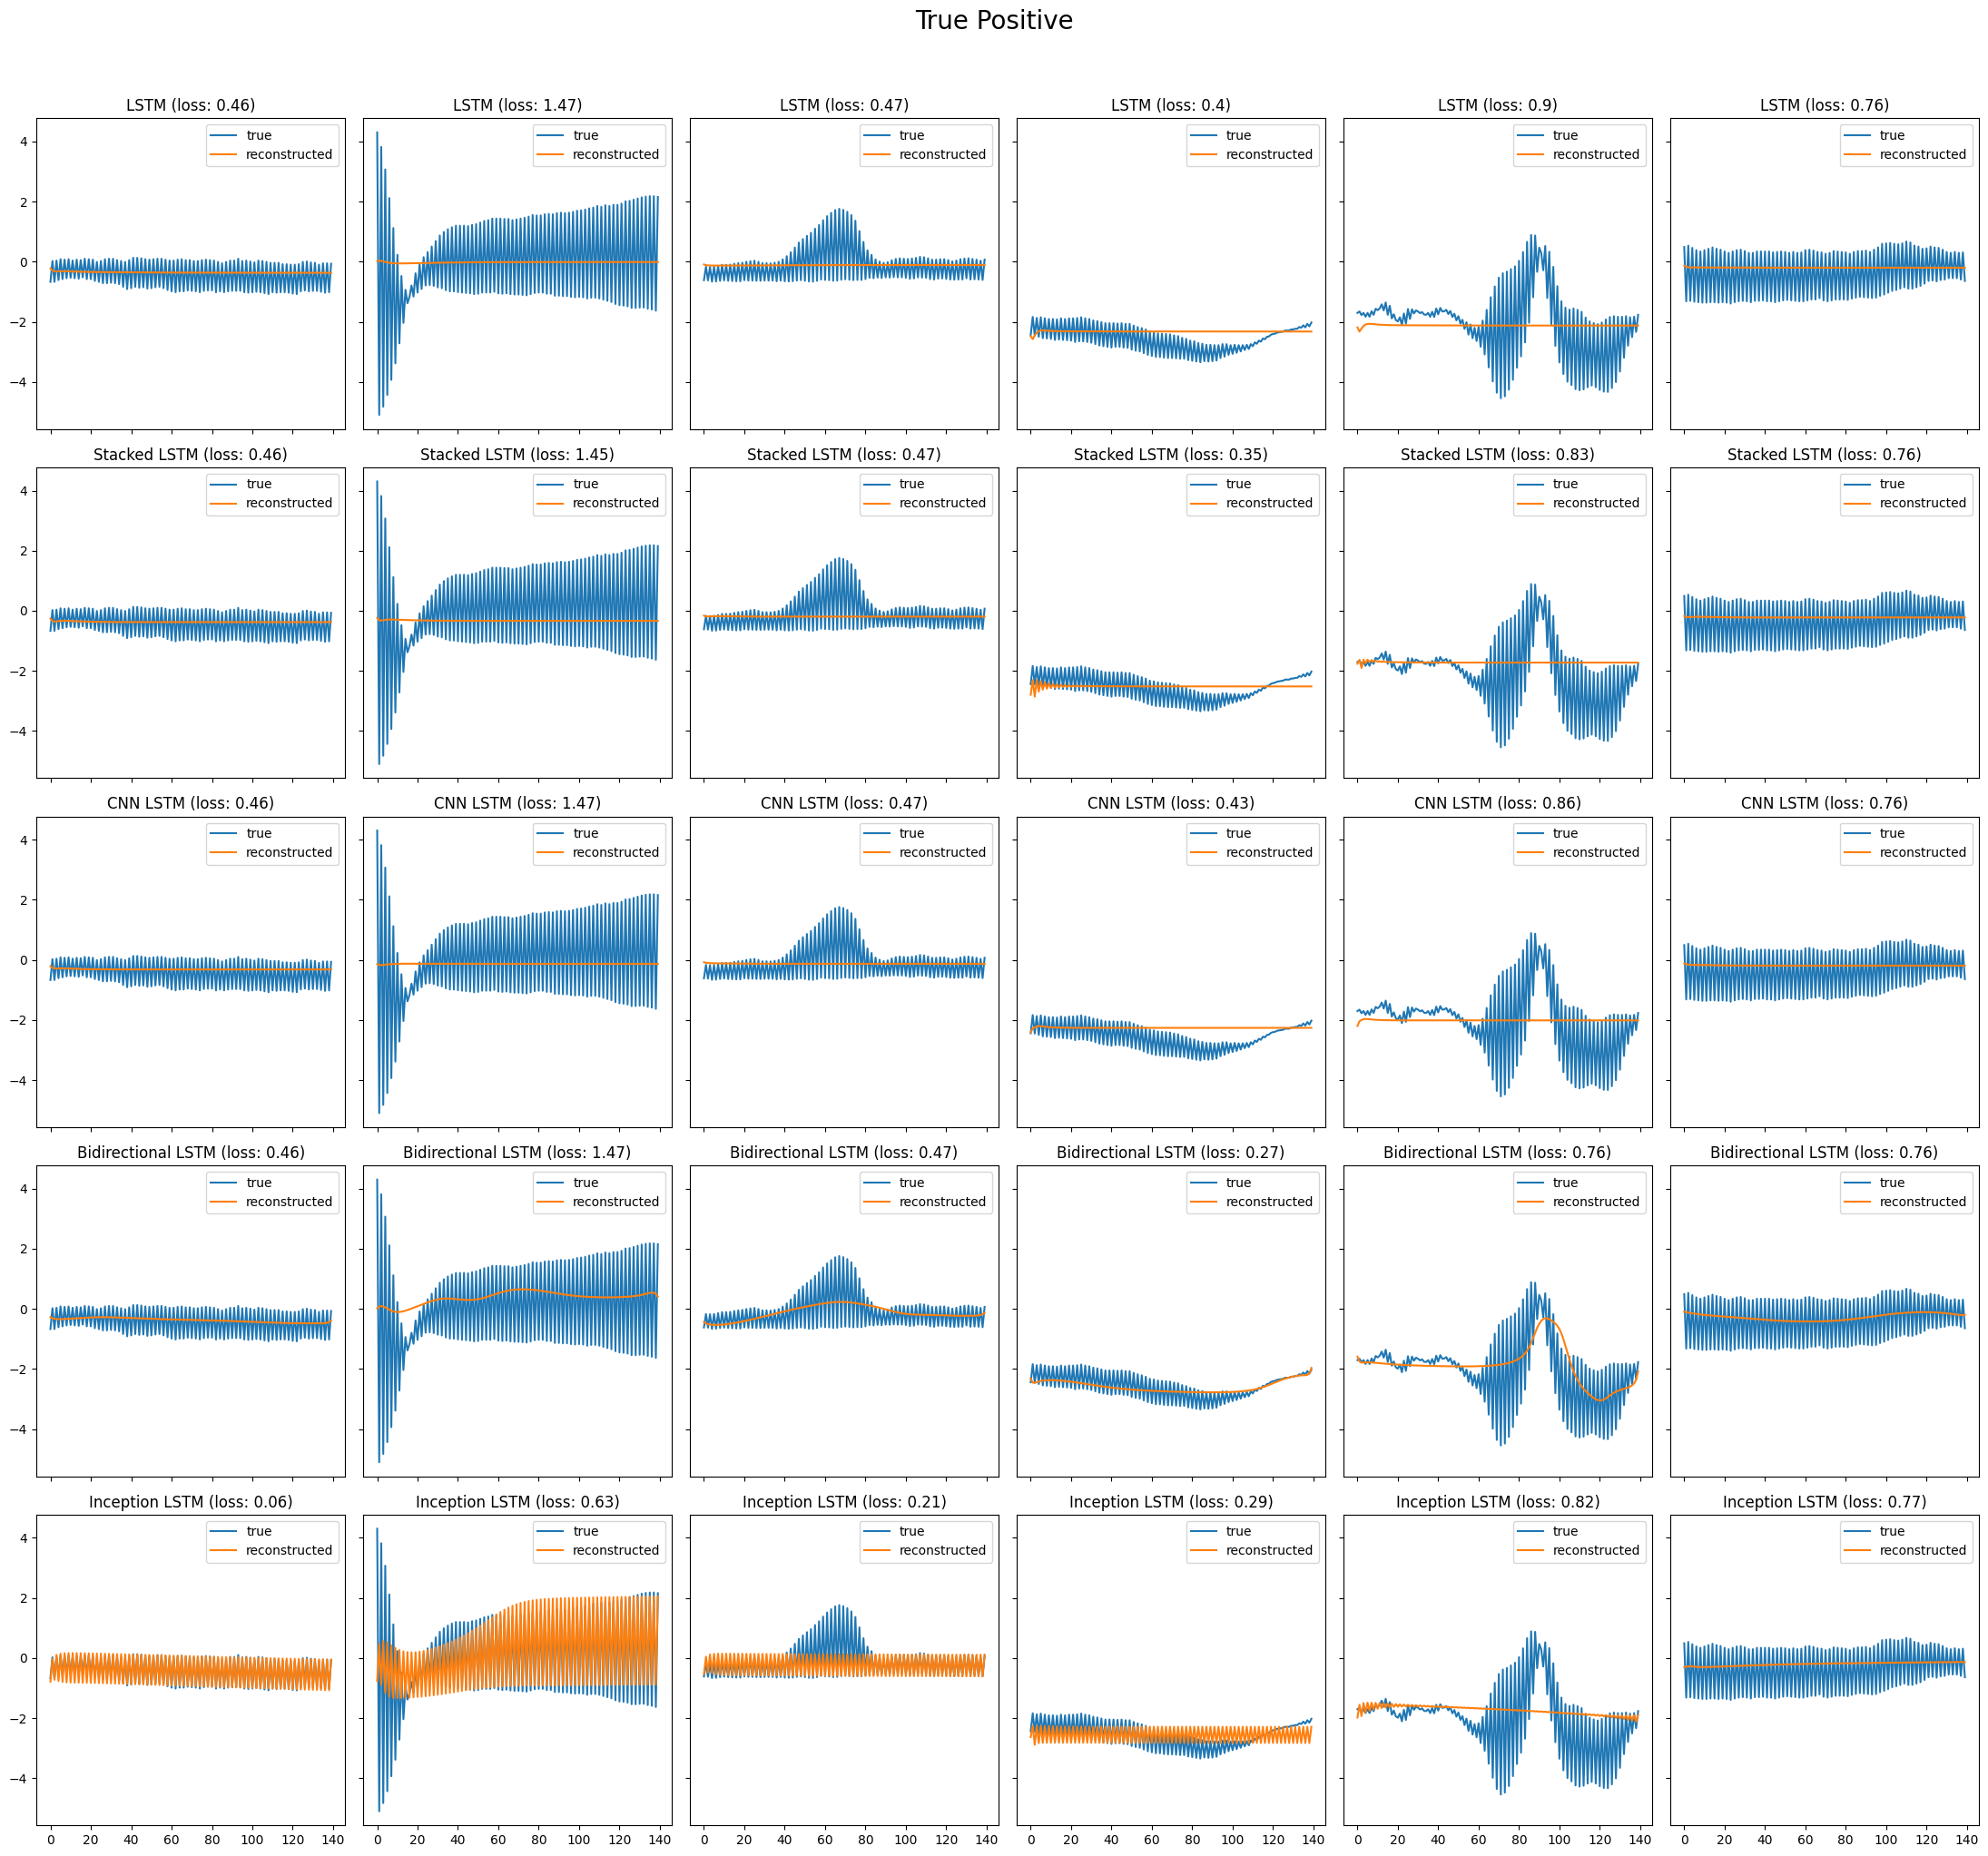
\includegraphics[width=0.35\textwidth]{MIT-BIH/TP.png}
        \caption{Compare true positive reconstructed sequences of mitbih(normal heartbeats sequences classified as normal)}
        \label{fig:image1}
    \end{figure}%
        \begin{figure}
        \centering
        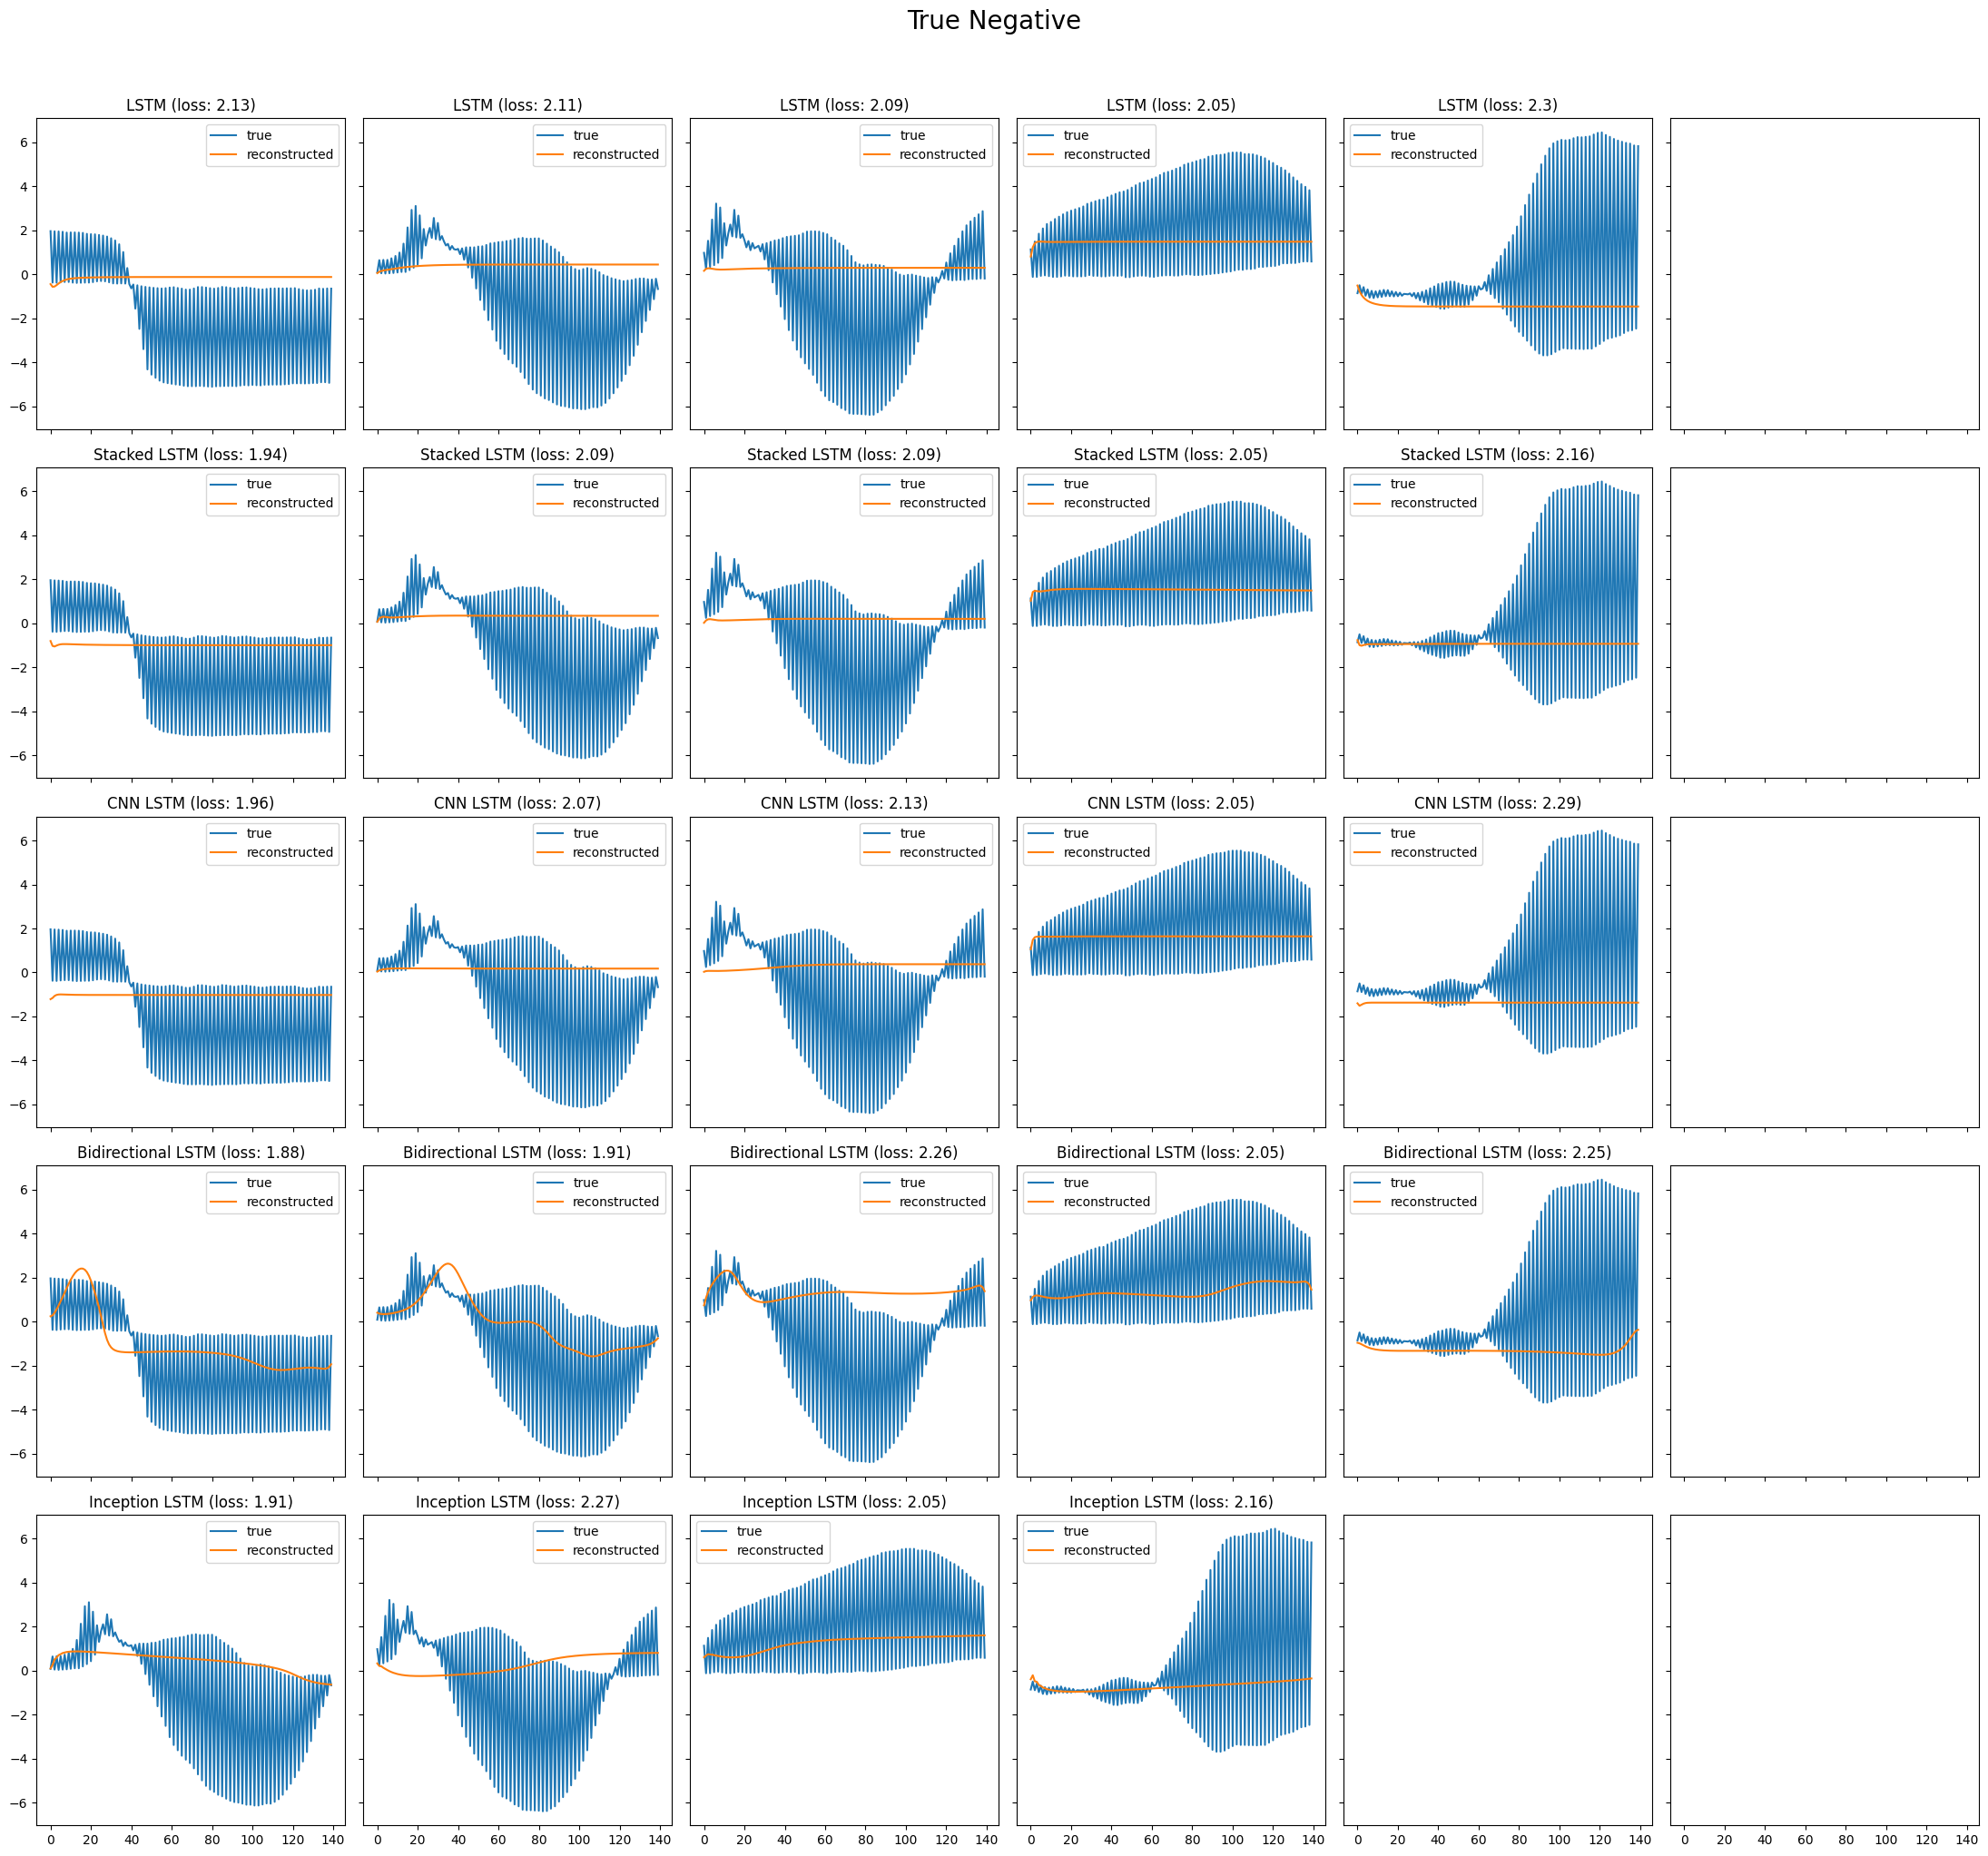
\includegraphics[width=0.35\textwidth]{MIT-BIH/TN.png}
        \caption{Compare true negative reconstructed sequences of mitbih(anomaly heartbeats sequences classified as anomaly)}
        \label{fig:image1}
    \end{figure}%
        \begin{figure}
        \centering
        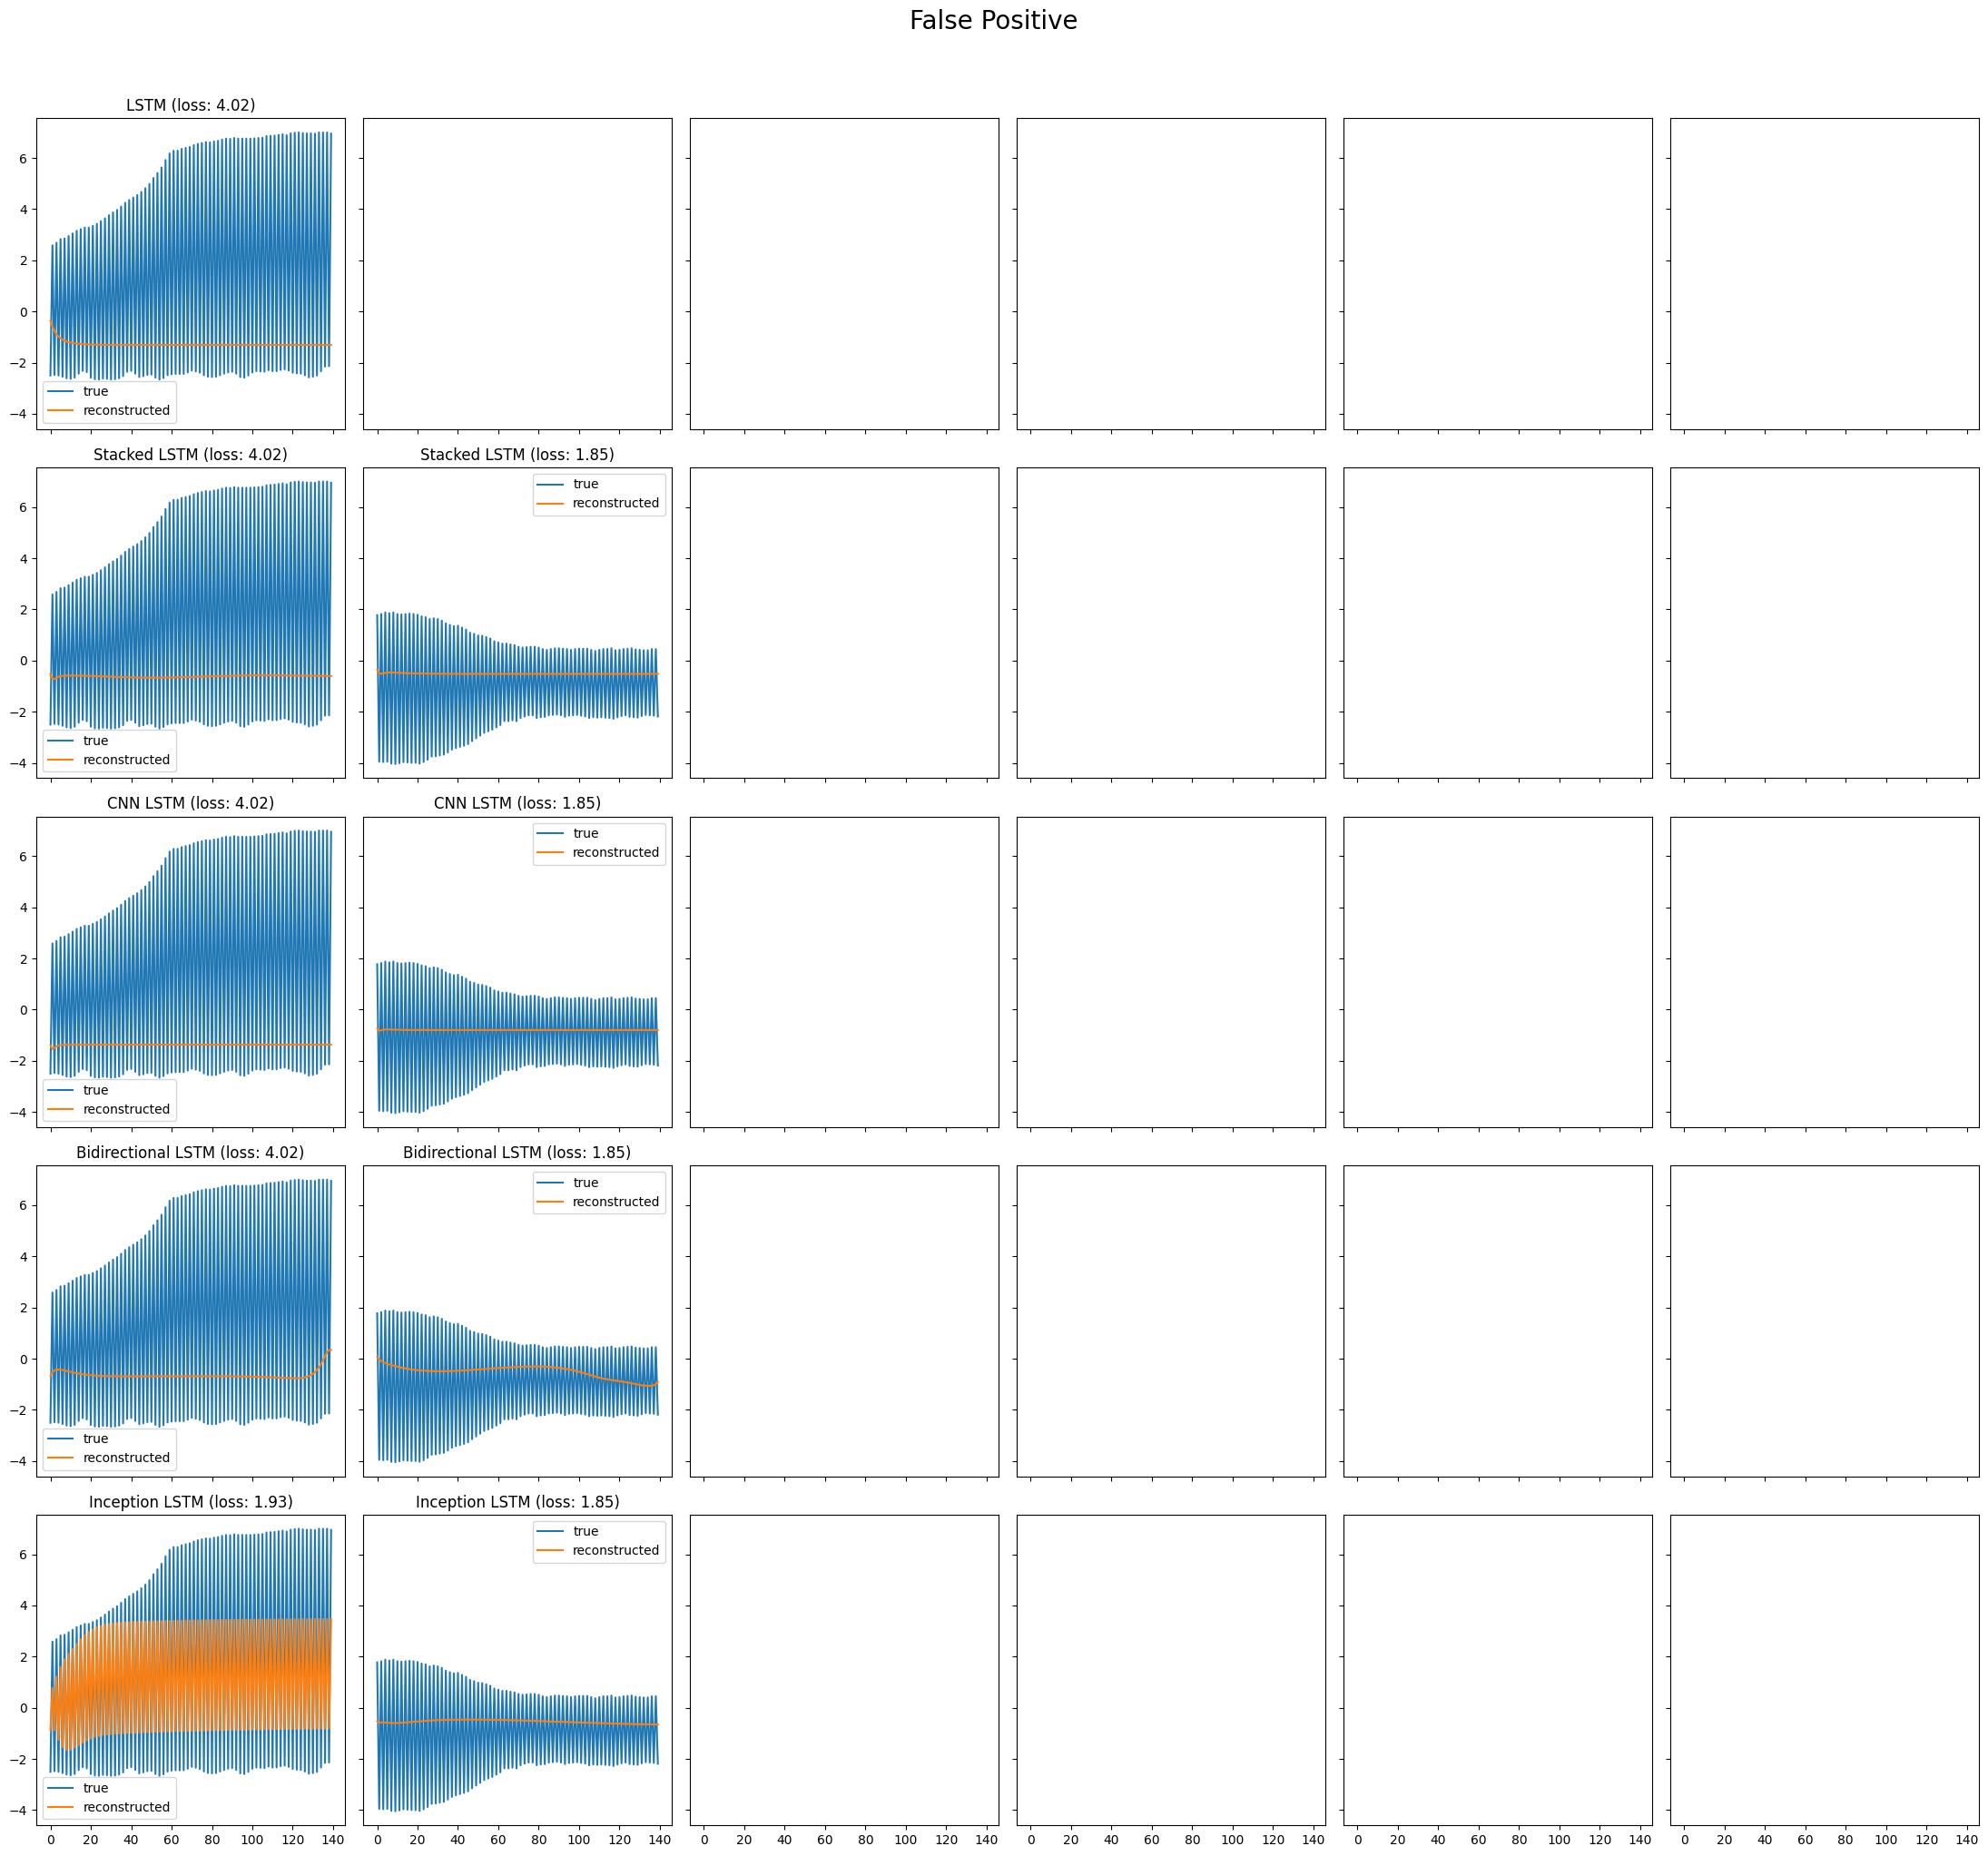
\includegraphics[width=0.35\textwidth]{MIT-BIH/FP.png}
        \caption{Compare false positive reconstructed sequences of mitbih(anomaly heartbeats sequences classified as normal)}
        \label{fig:image1}
    \end{figure}%
        \begin{figure}
        \centering
        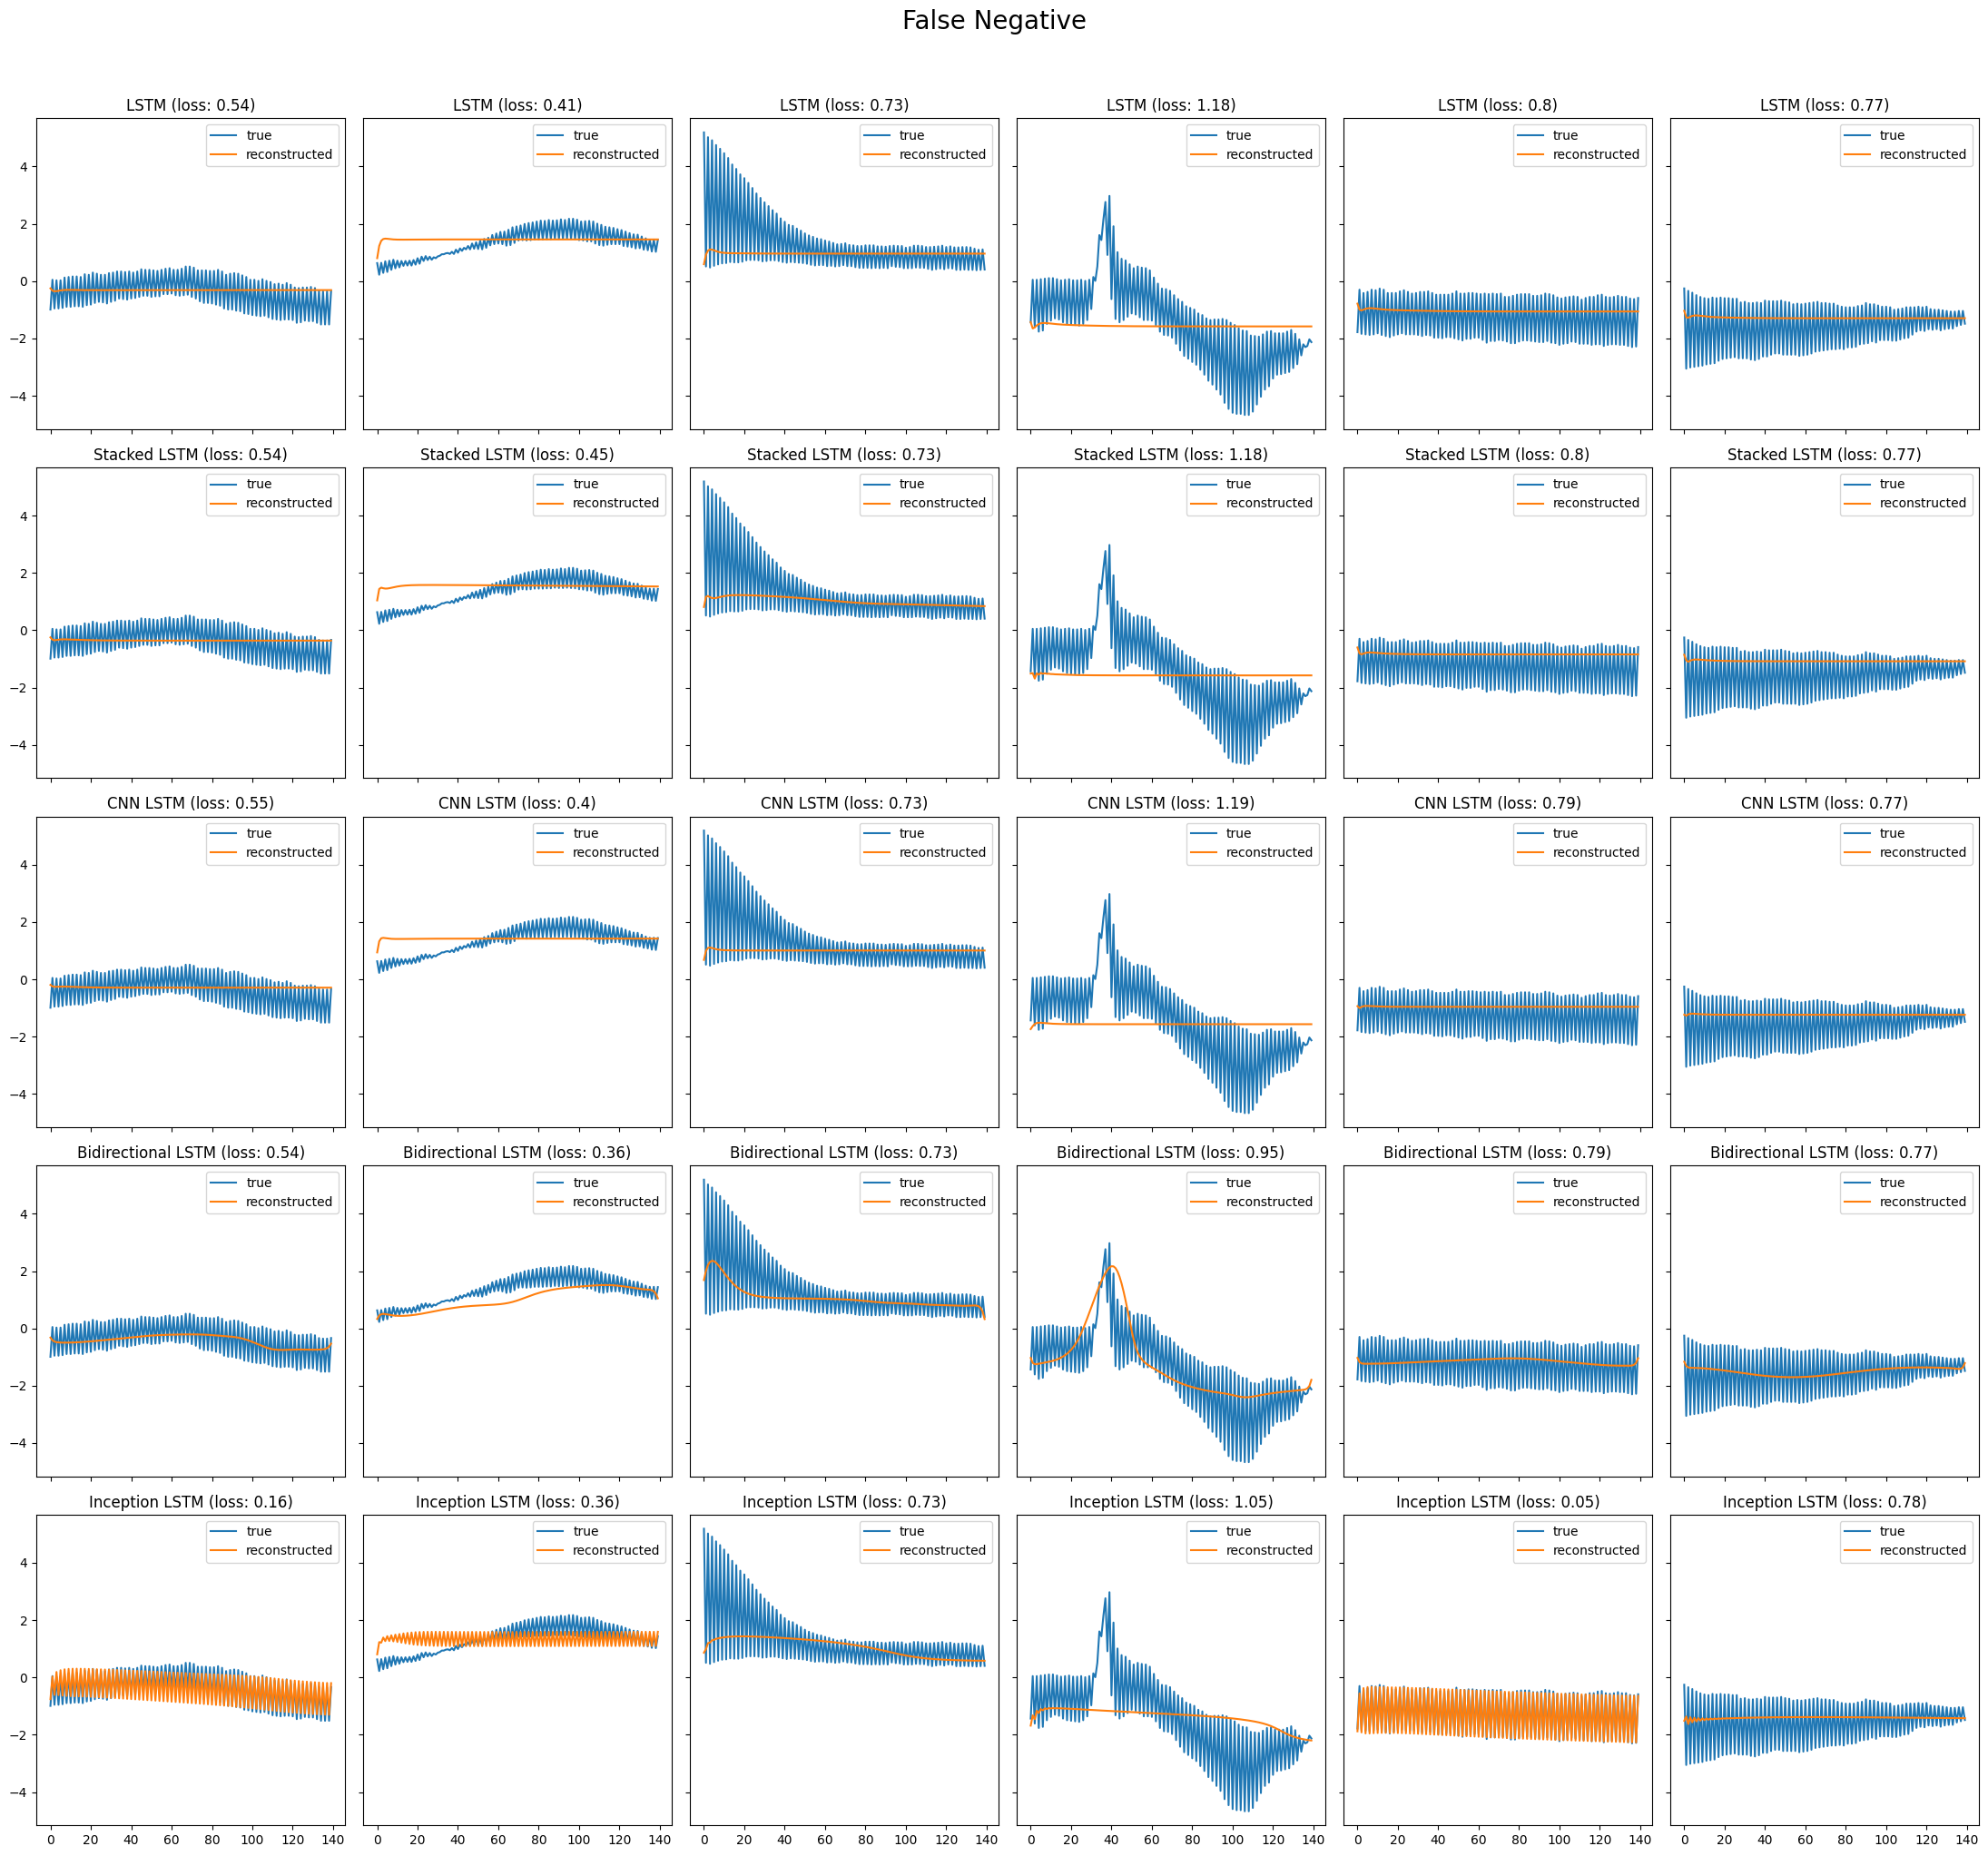
\includegraphics[width=0.35\textwidth]{MIT-BIH/FN.png}
        \caption{Compare false negative reconstructed sequences of mitbih(normal heartbeats sequences classified as anomaly)}
        \label{fig:image1}
    \end{figure}%

% \begin{figure*}[ht]
%     \centering
%     % First row
%     \begin{subfigure}{0.4\textwidth}
%         \centering
%         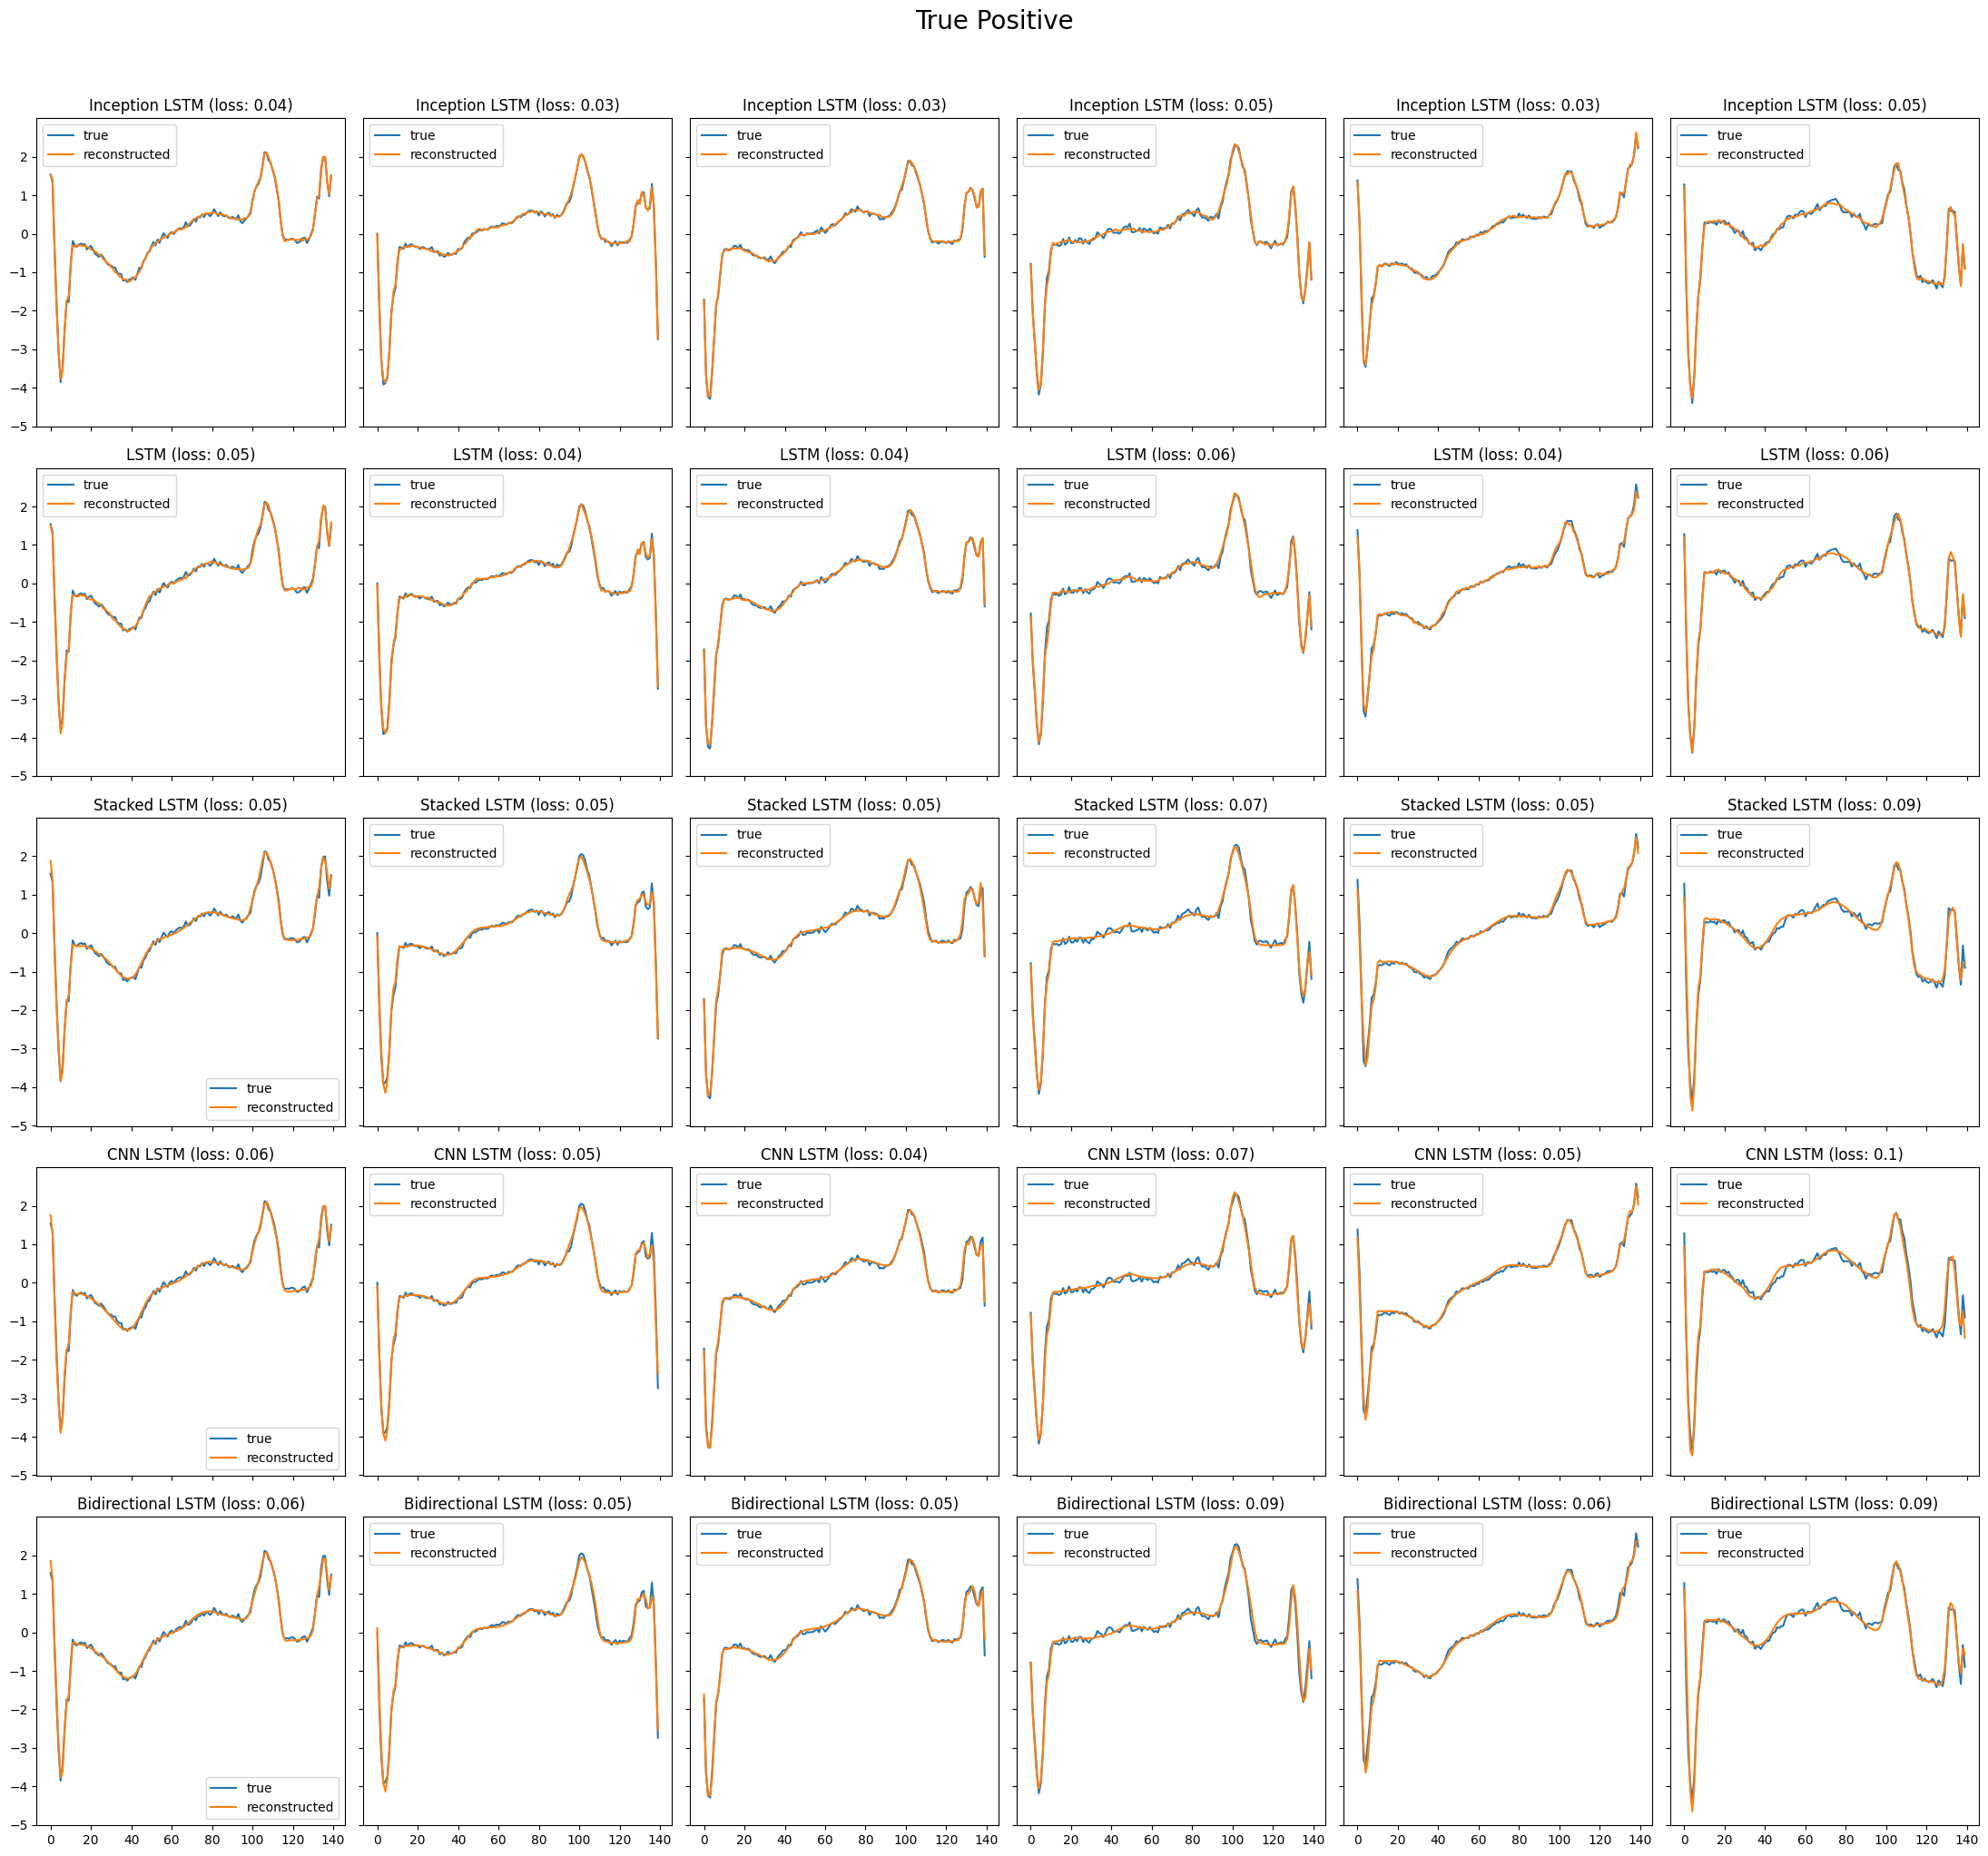
\includegraphics[width=\linewidth]{ecg5000/TP.png}
%         \caption{Compare true positive reconstructed sequences (normal heartbeats sequences classified as normal)}
%         \label{fig:image1}
%     \end{subfigure}%
%     \hfill
%     \begin{subfigure}{0.4\textwidth}
%         \centering
%         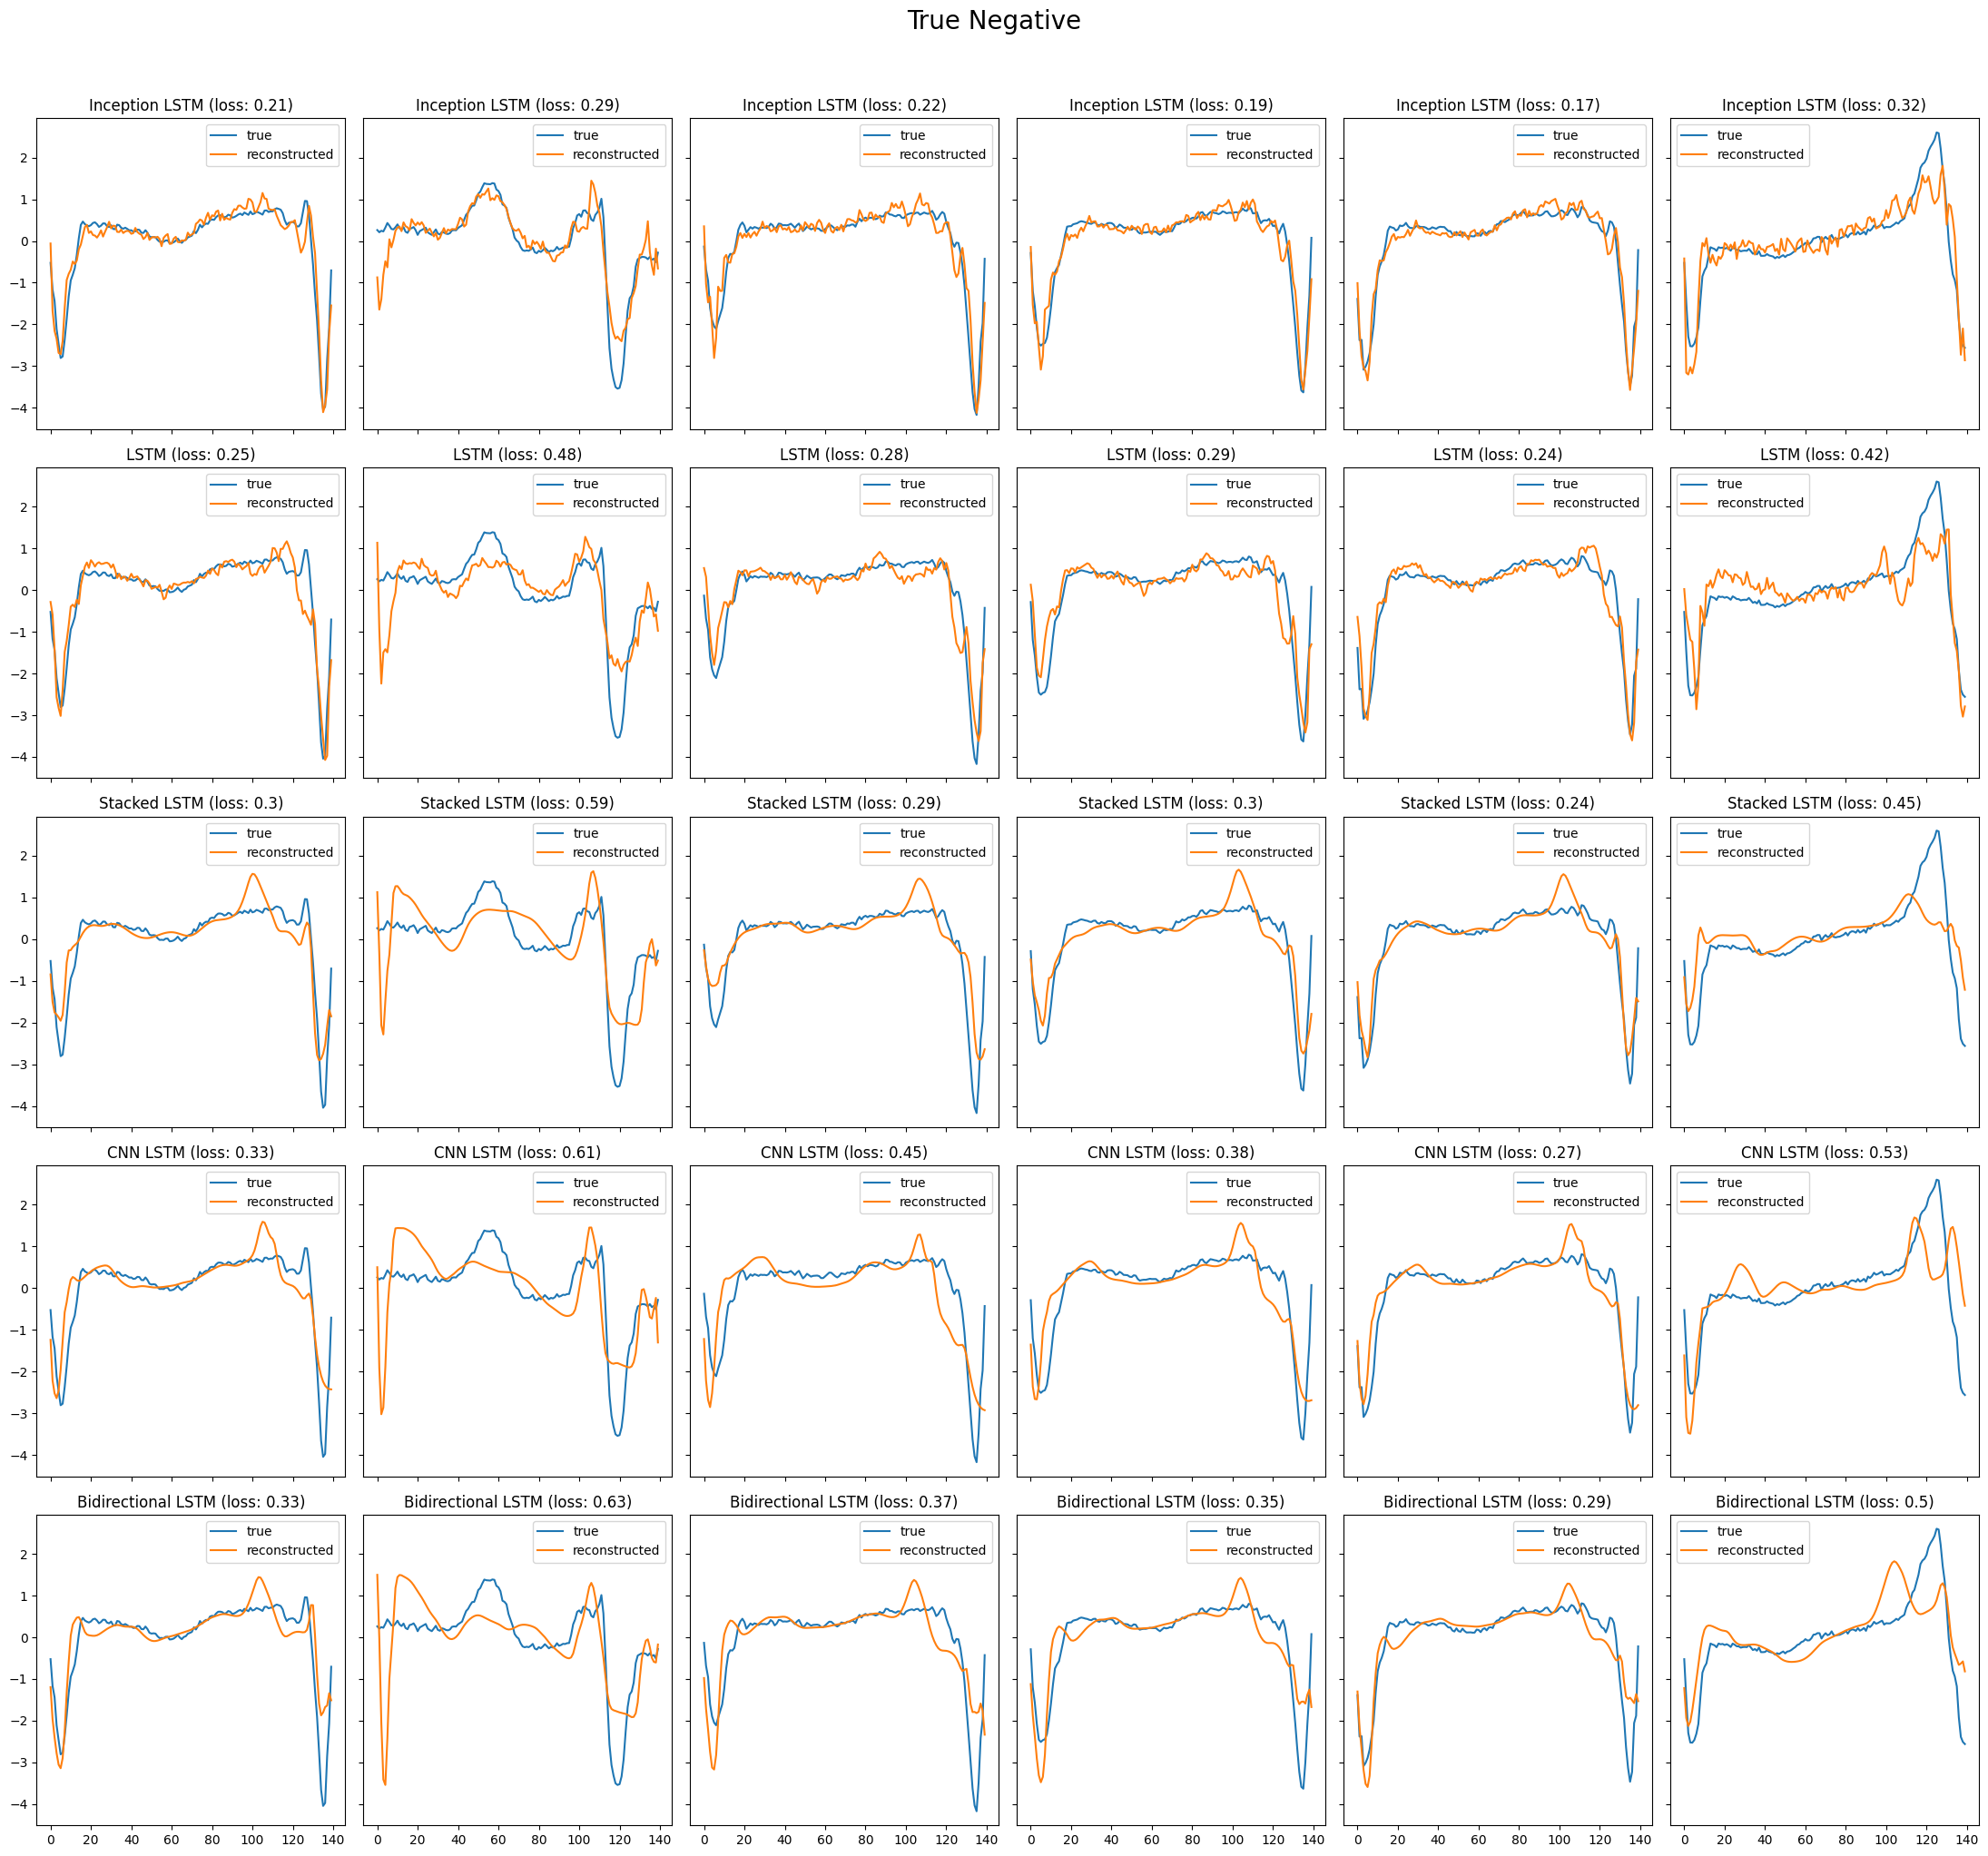
\includegraphics[width=\linewidth]{ecg5000/TN.png}
%         \caption{Compare true negative reconstructed sequences (anomaly heartbeats sequences classified as anomaly)}
%         \label{fig:image2}
%     \end{subfigure}

%     % Second row
%     \vspace{0.5cm} % Optional space between rows
%     \begin{subfigure}{0.4\textwidth}
%         \centering
%         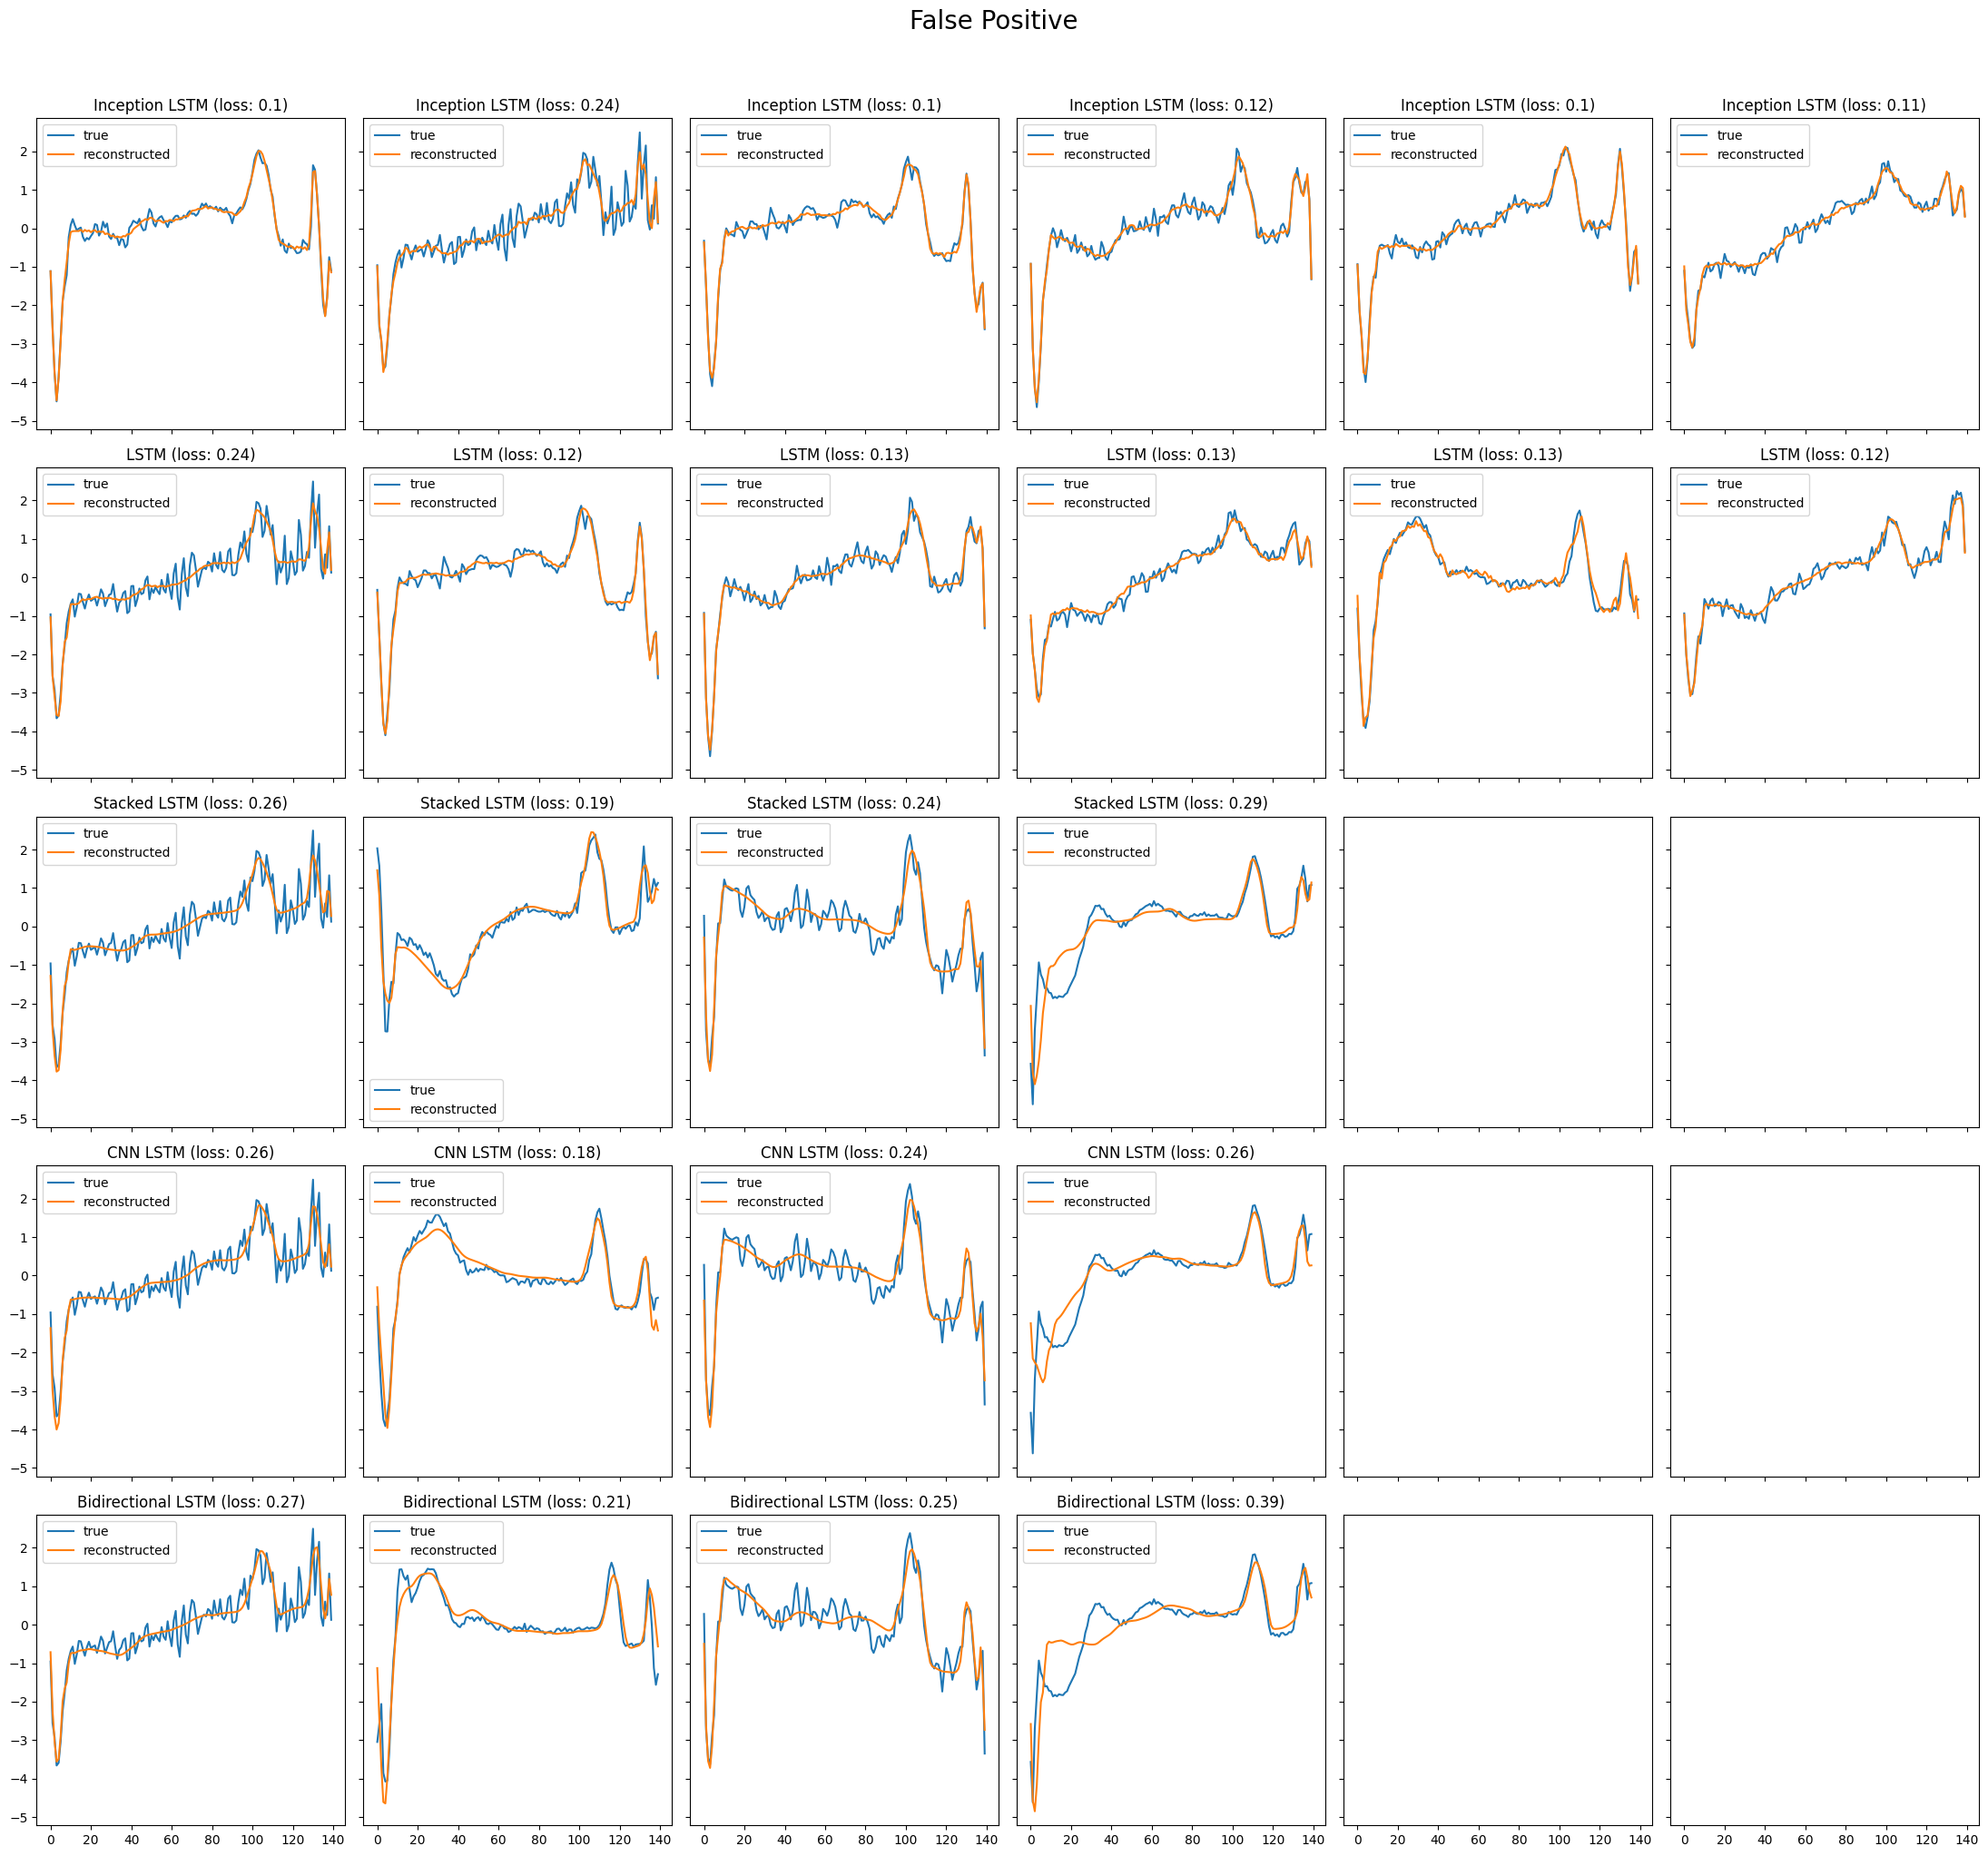
\includegraphics[width=\linewidth]{ecg5000/FP.png}
%         \caption{Compare false positive reconstructed sequences (anomaly heartbeats sequences classified as normal)}
%         \label{fig:image3}
%     \end{subfigure}%
%     \hfill
%     \begin{subfigure}{0.4\textwidth}
%         \centering
%         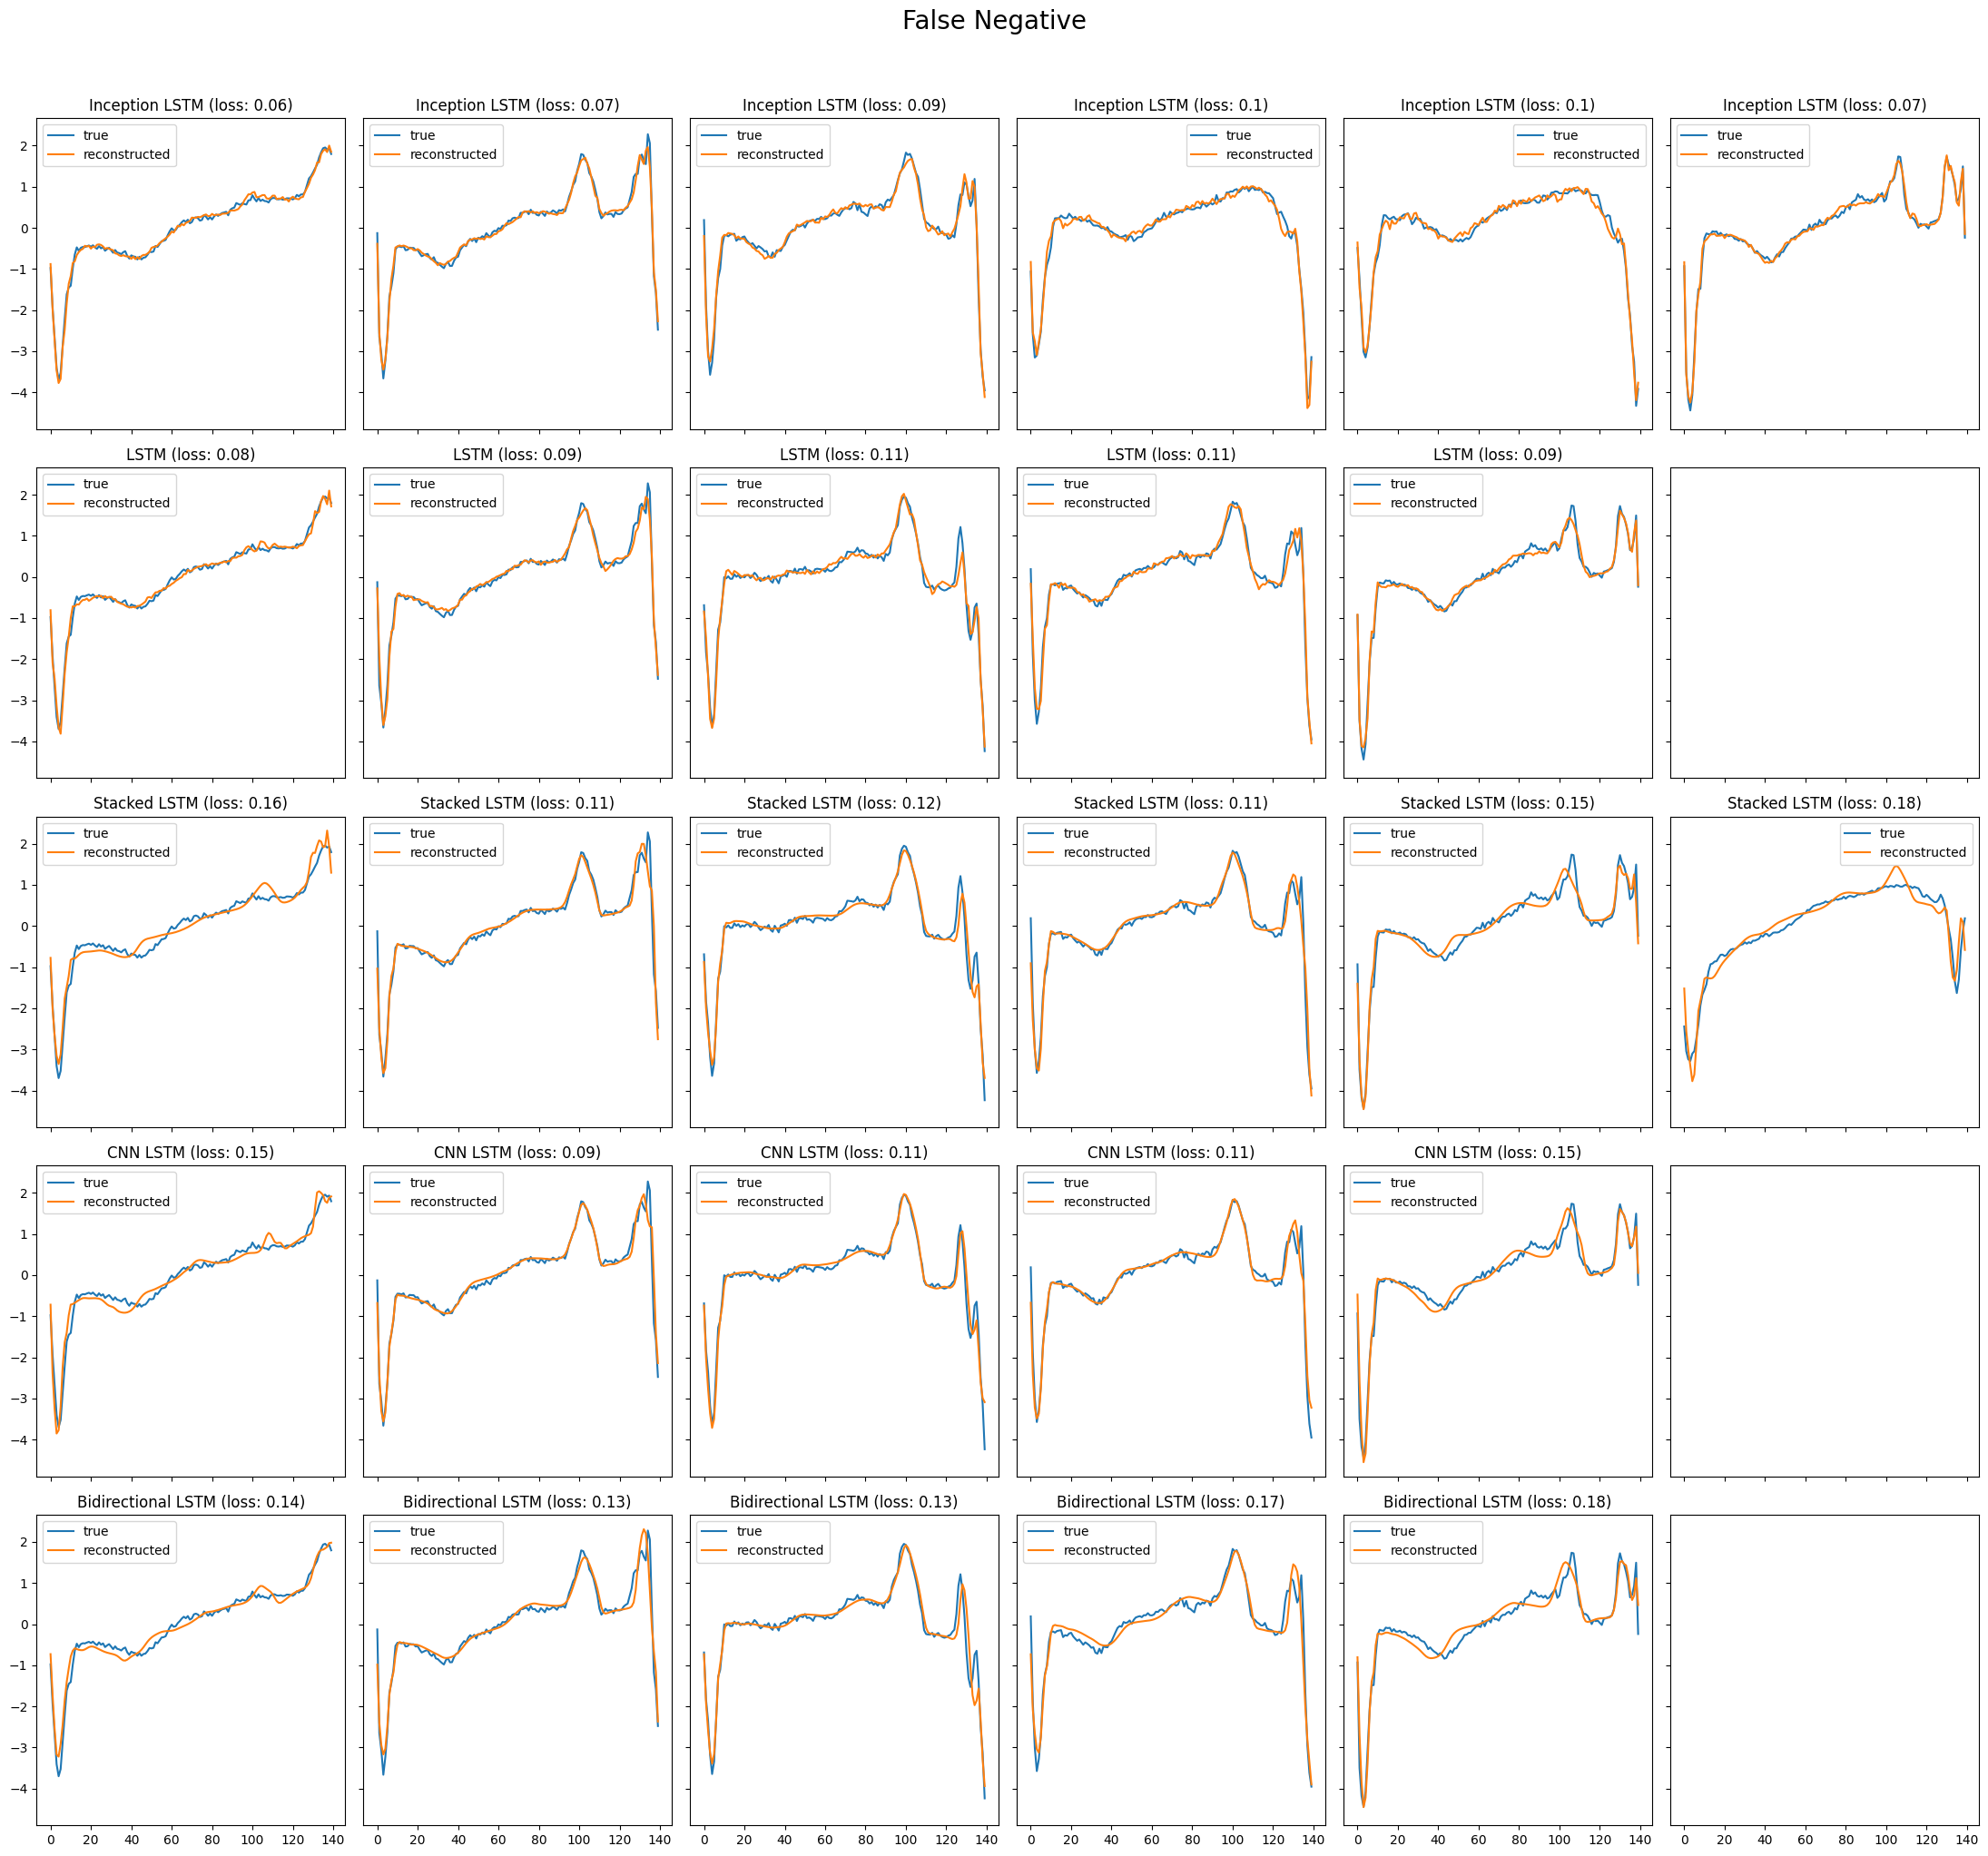
\includegraphics[width=\linewidth]{ecg5000/FN.png}
%         \caption{Compare false negative reconstructed sequences (normal heartbeats sequences classified as anomlay)}
%         \label{fig:image4}
%     \end{subfigure}

%     \caption{Plot Prediction for ECG5000}
%     \label{fig:main}
% \end{figure*}

% Please add the following required packages to your document preamble:
% \usepackage[table,xcdraw]{xcolor}
% Beamer presentation requires \usepackage{colortbl} instead of \usepackage[table,xcdraw]{xcolor}



% \begin{figure*}[ht]
%     \centering
%     % First row
%     \begin{subfigure}{0.4\textwidth}
%         \centering
%         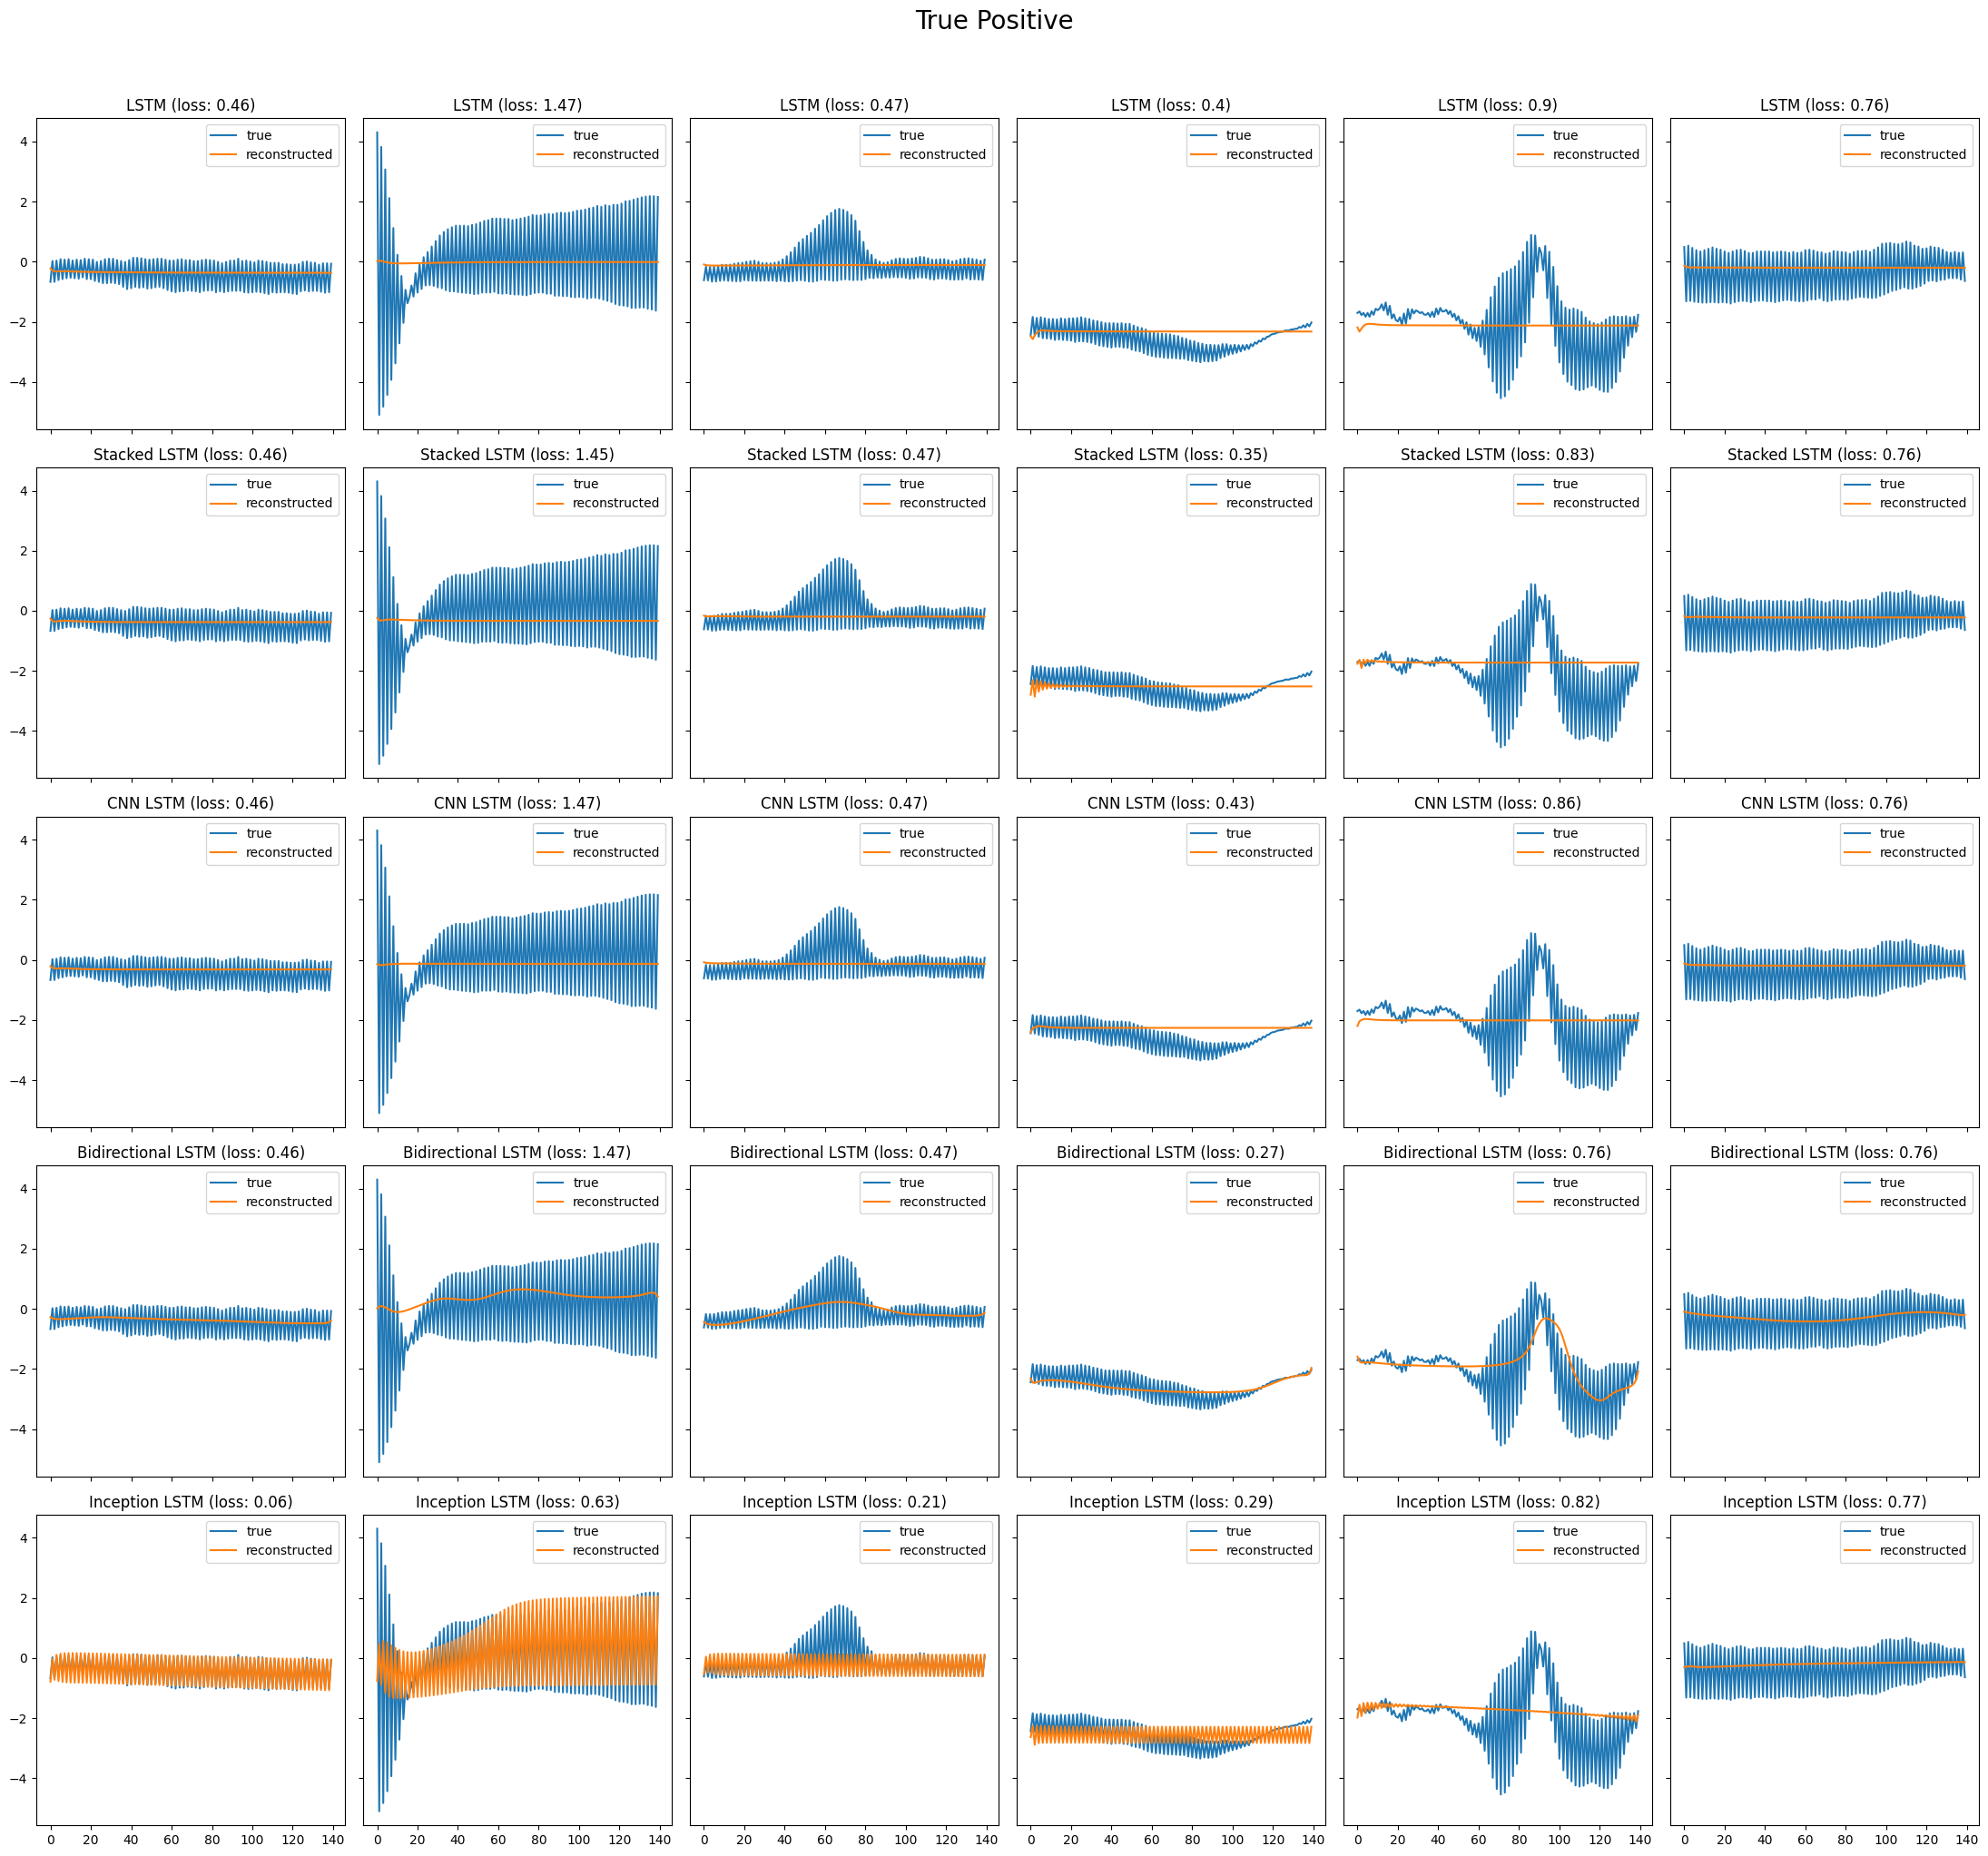
\includegraphics[width=\linewidth]{MIT-BIH/TP.png}
%         \caption{Compare true positive reconstructed sequences (normal heartbeats sequences classified as normal)}
%         \label{fig:image1}
%     \end{subfigure}%
%     \hfill
%     \begin{subfigure}{0.4\textwidth}
%         \centering
%         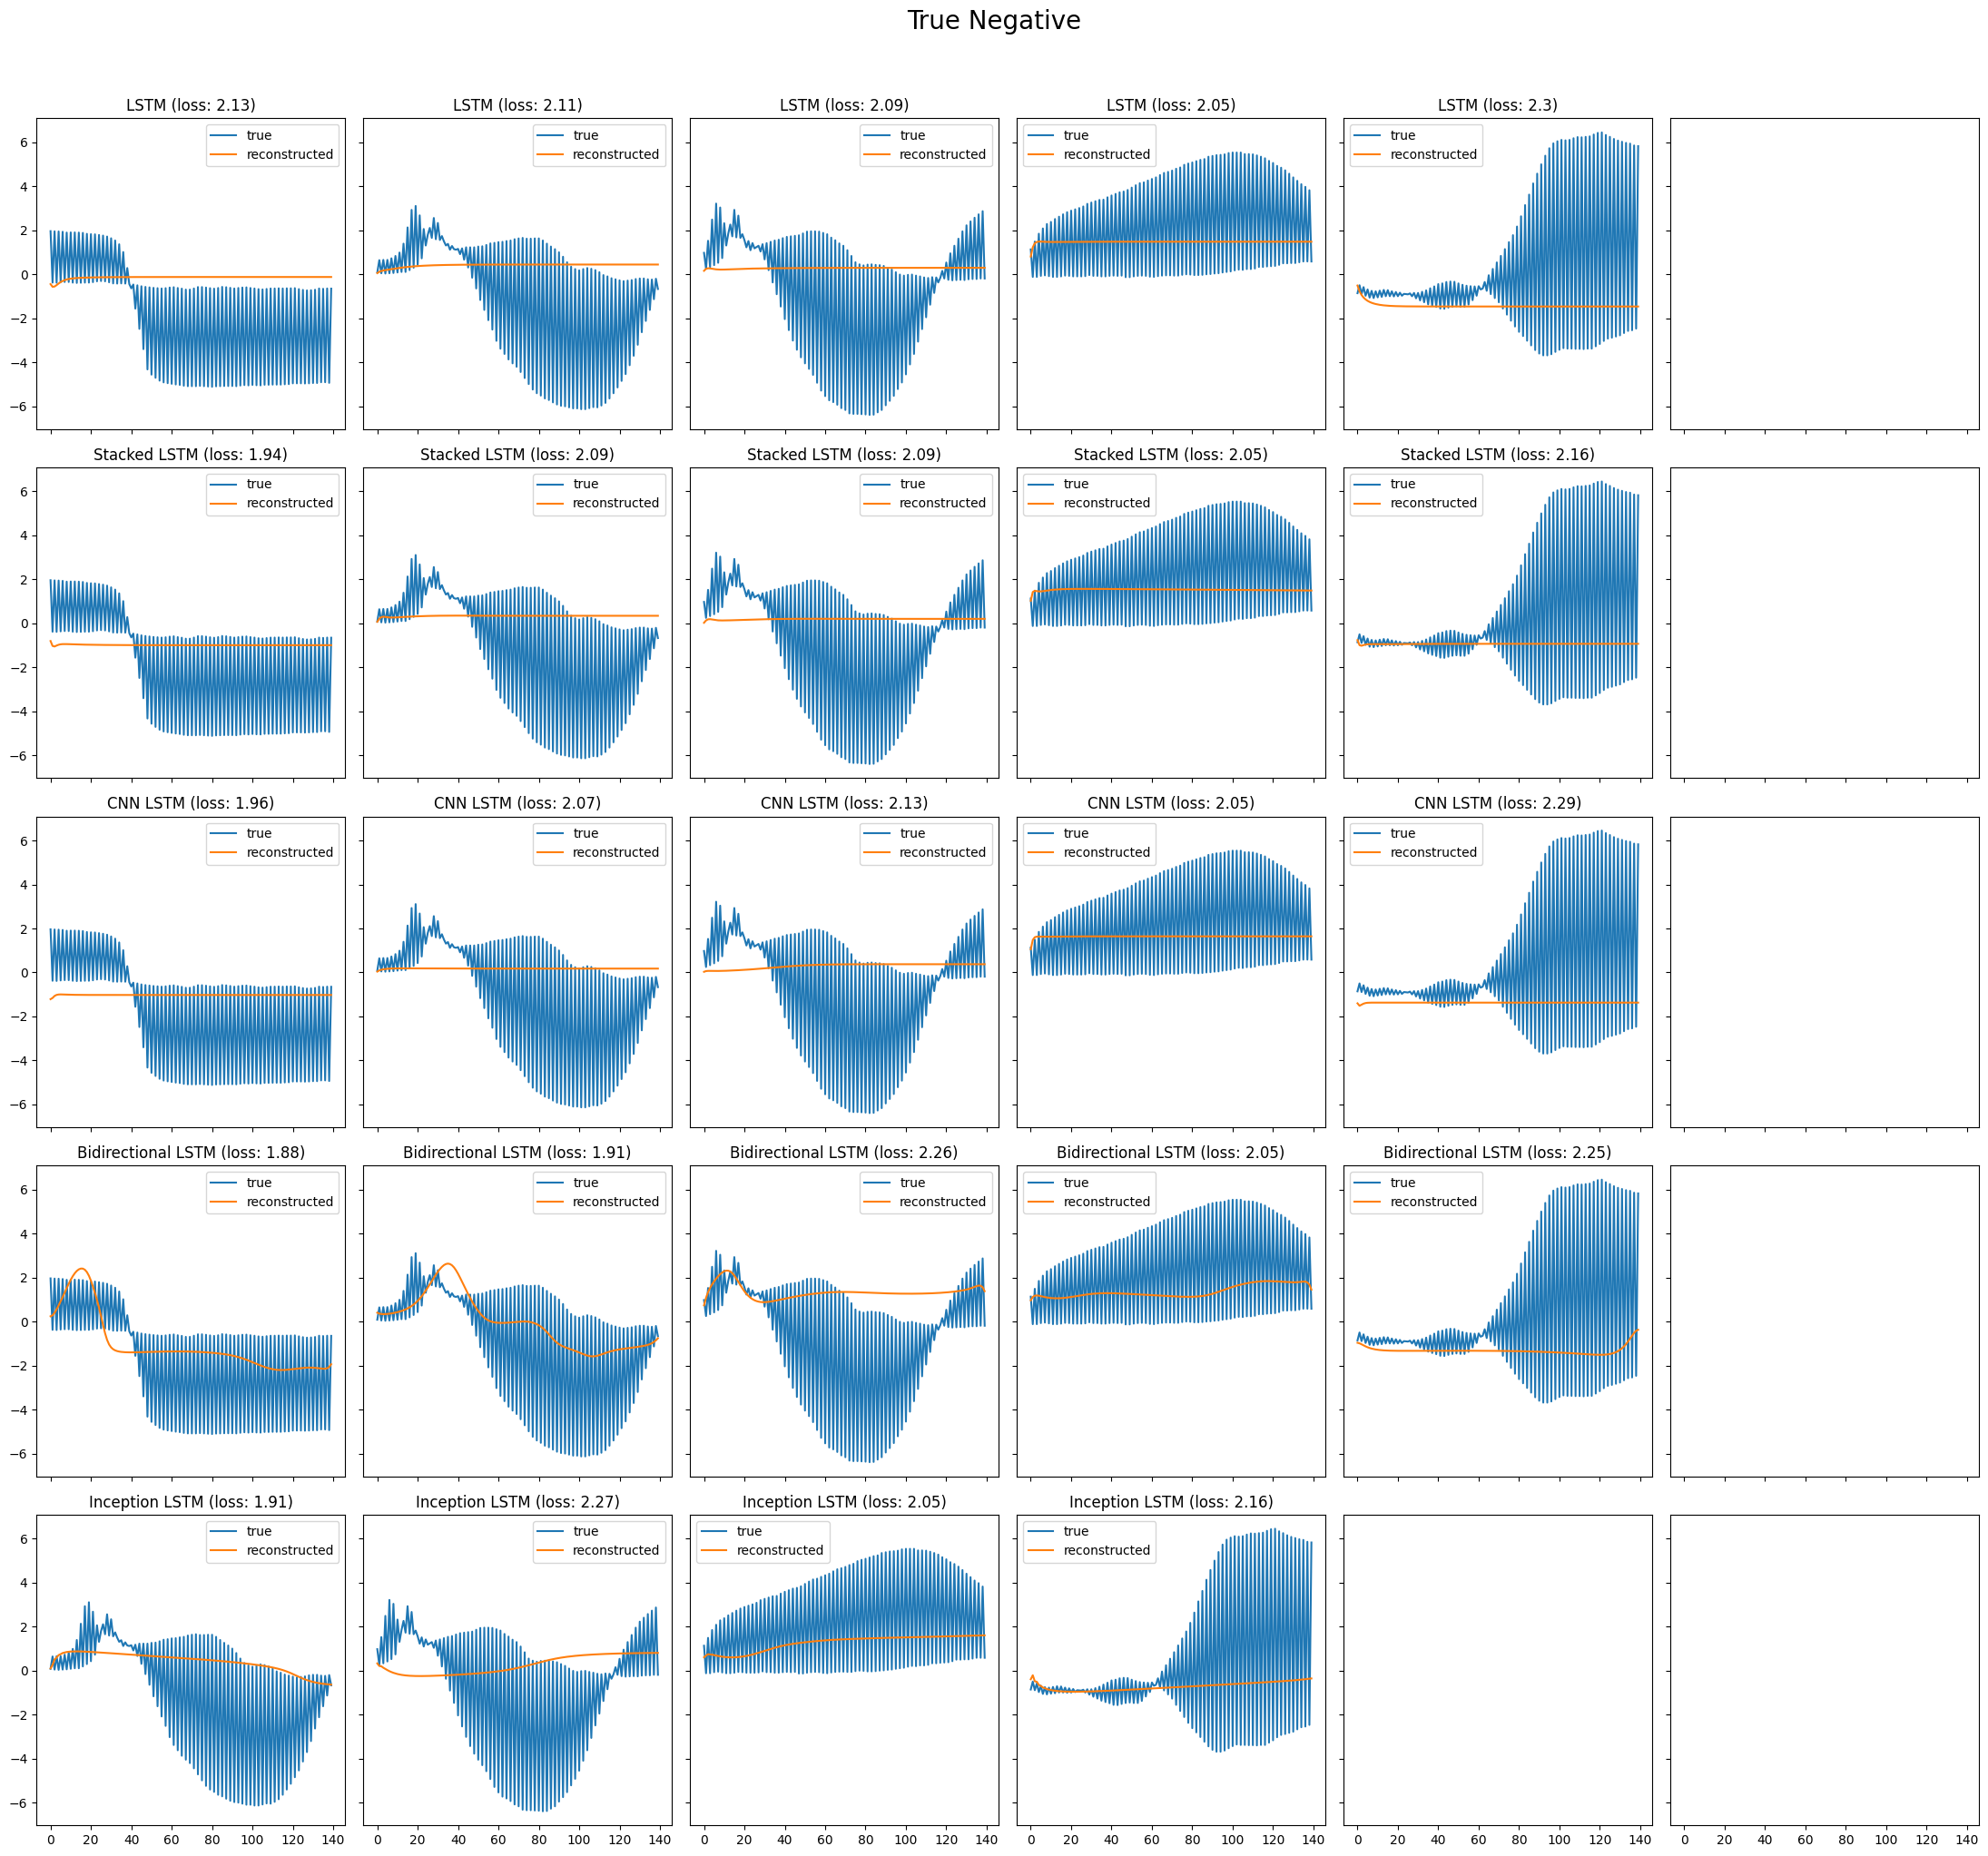
\includegraphics[width=\linewidth]{MIT-BIH/TN.png}
%         \caption{Compare true negative reconstructed sequences (anomaly heartbeats sequences classified as anomaly)}
%         \label{fig:image2}
%     \end{subfigure}

%     % Second row
%     \vspace{0.5cm} % Optional space between rows
%     \begin{subfigure}{0.4\textwidth}
%         \centering
%         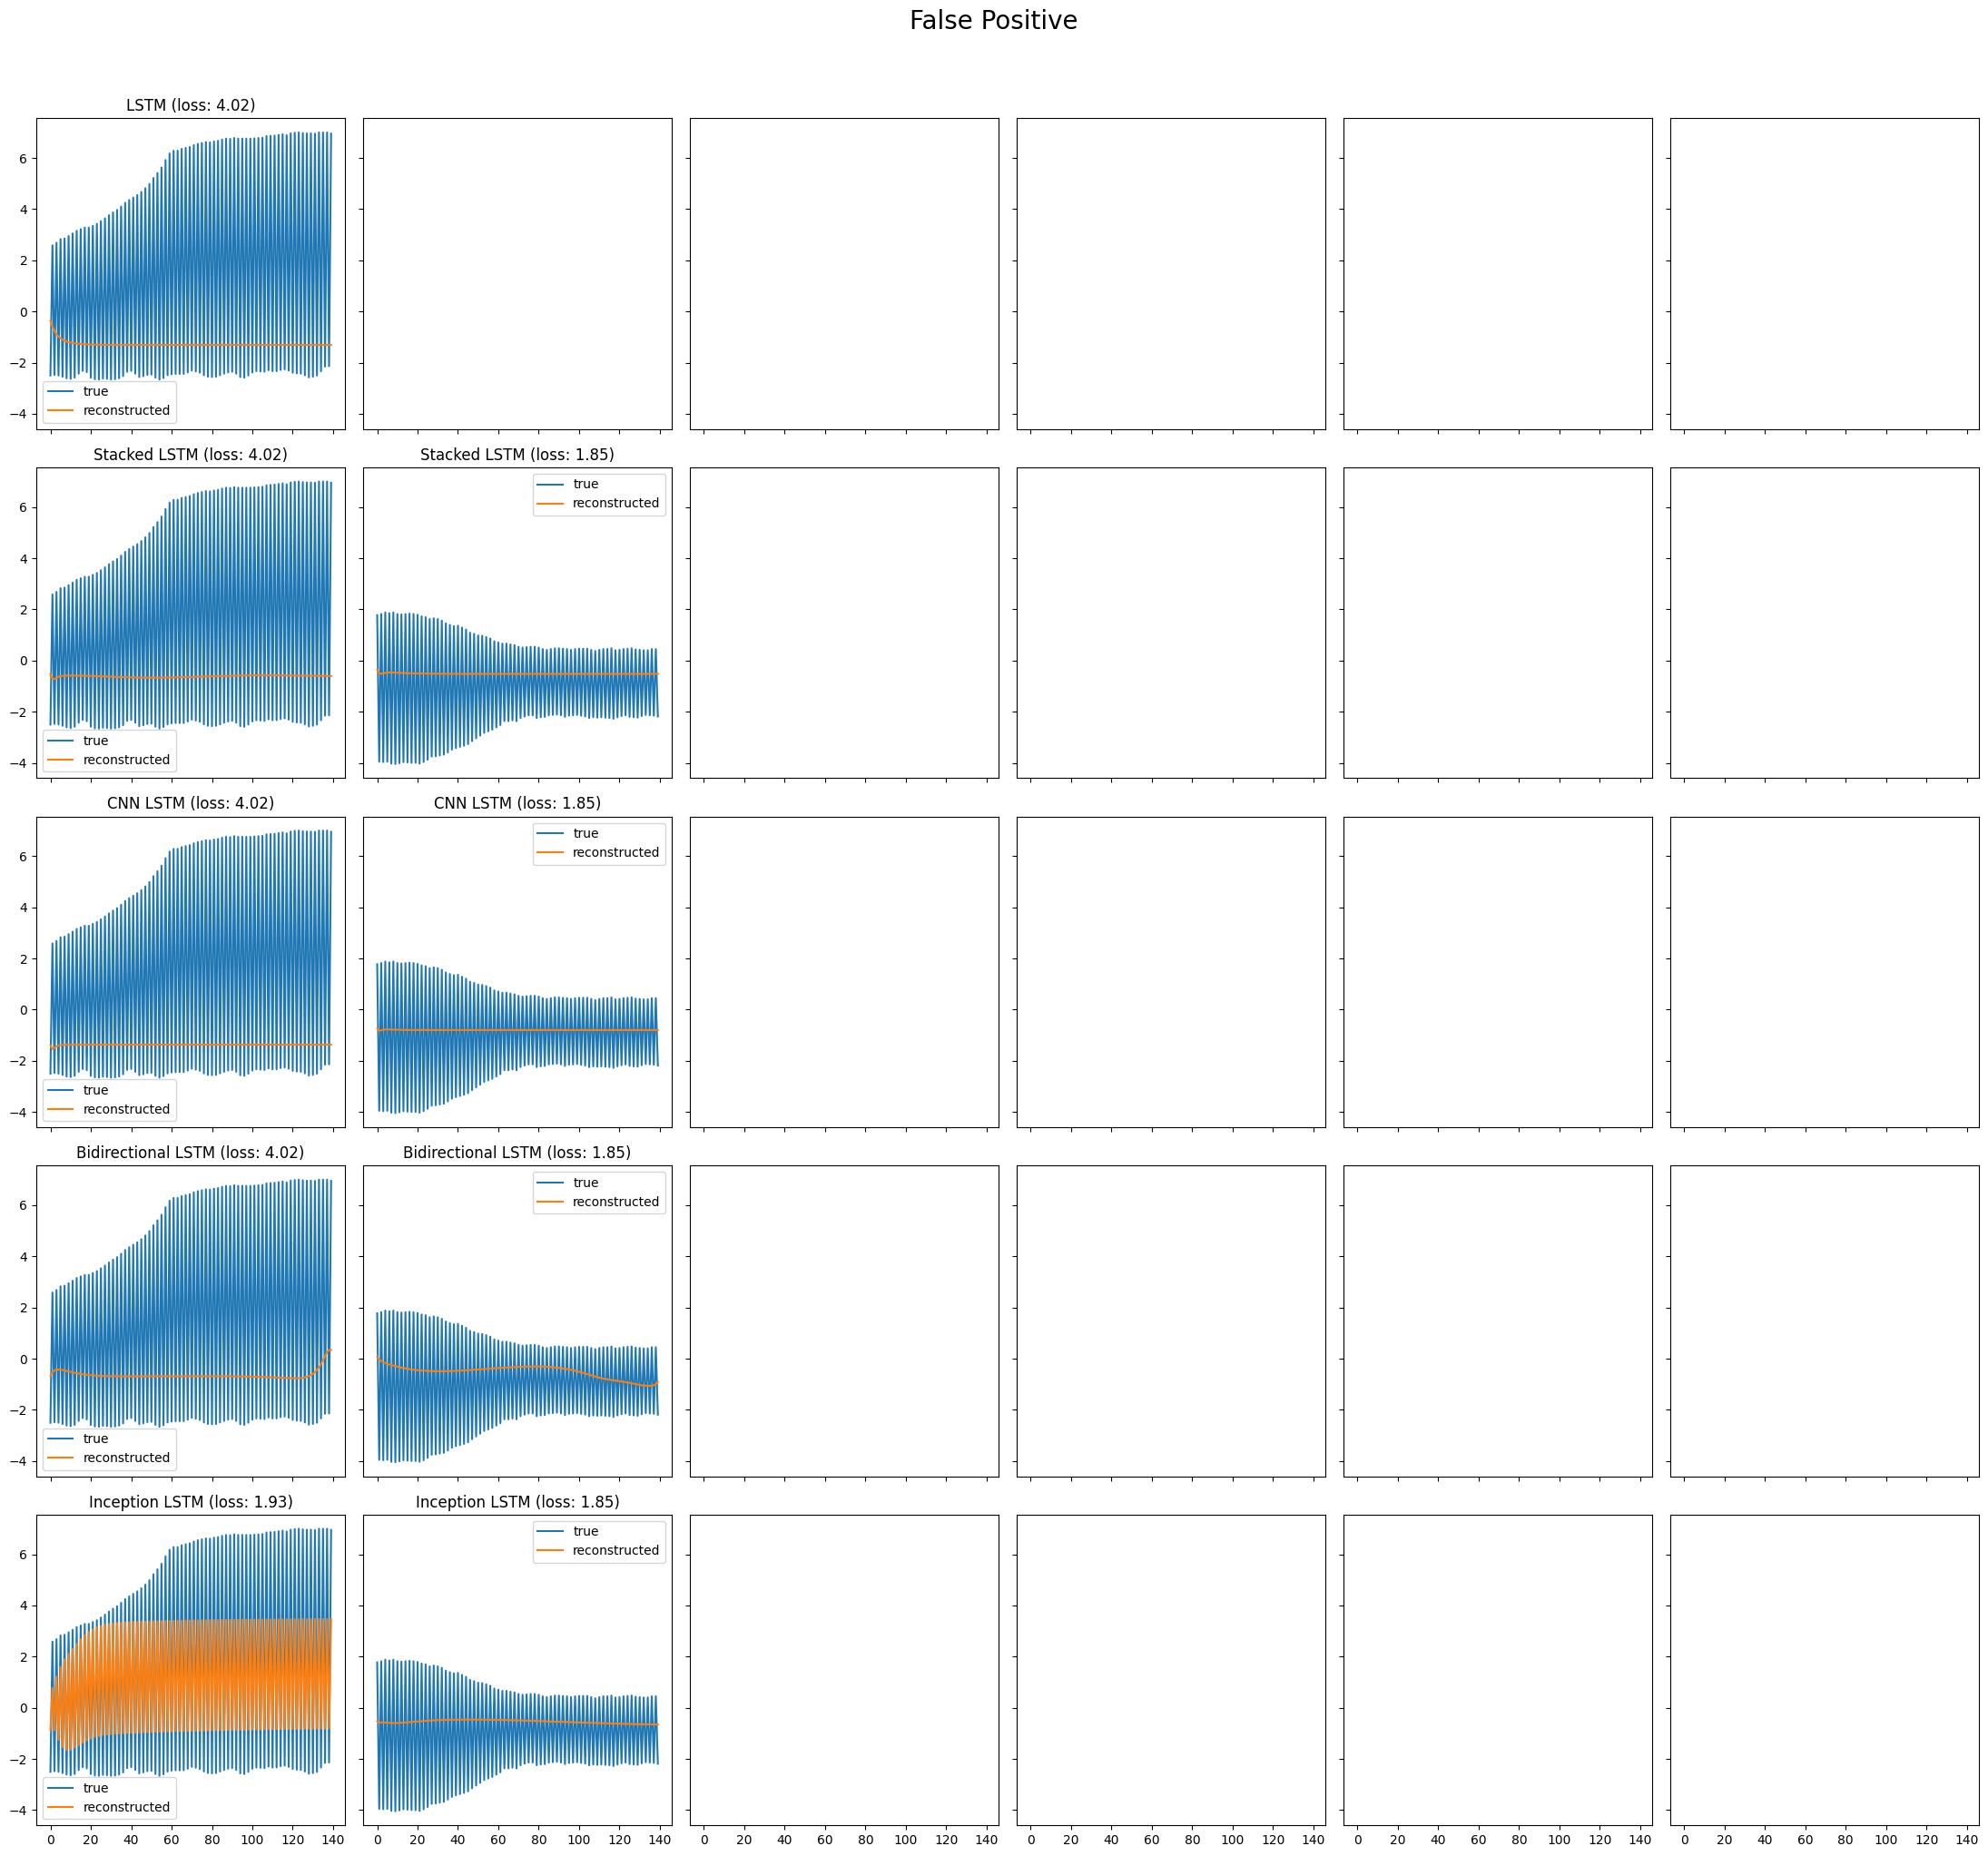
\includegraphics[width=\linewidth]{MIT-BIH/FP.png}
%         \caption{Compare false positive reconstructed sequences (anomaly heartbeats sequences classified as normal)}
%         \label{fig:image3}
%     \end{subfigure}%
%     \hfill
%     \begin{subfigure}{0.4\textwidth}
%         \centering
%         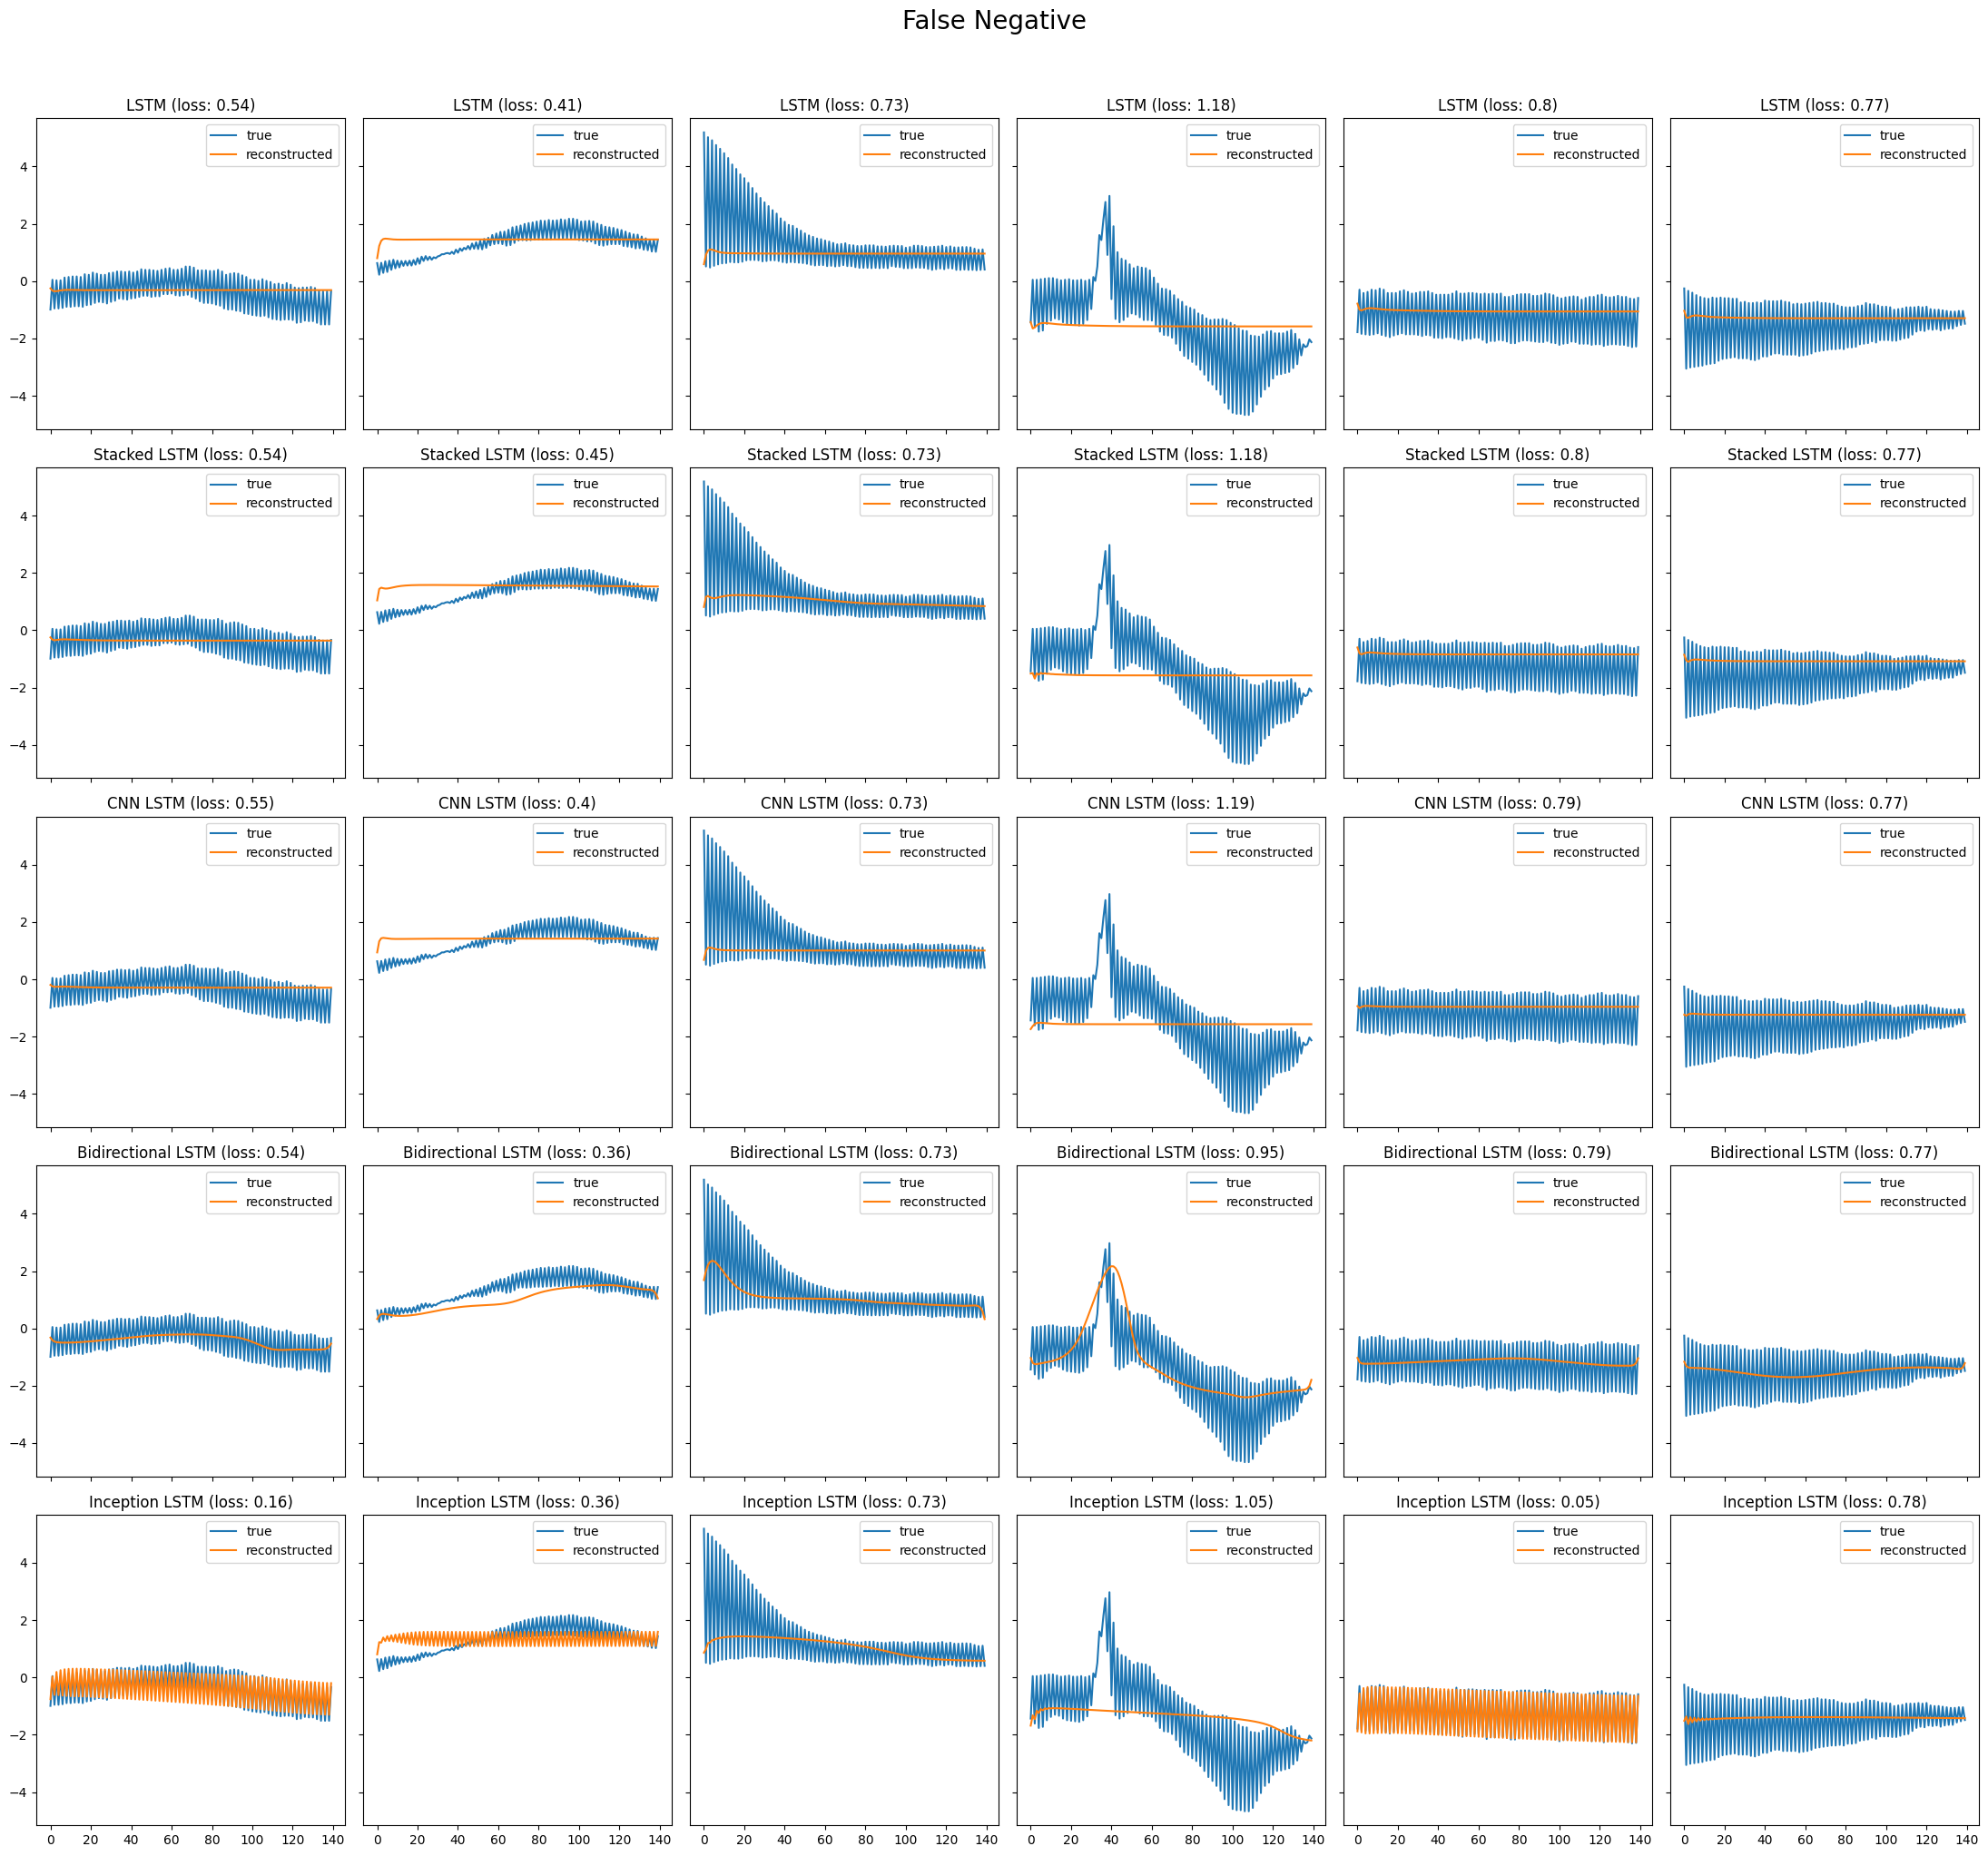
\includegraphics[width=\linewidth]{MIT-BIH/FN.png}
%         \caption{Compare false negative reconstructed sequences (normal heartbeats sequences classified as anomlay)}
%         \label{fig:image4}
%     \end{subfigure}

%     \caption{Plot Prediction for MIT-BIH}
%     \label{fig:main}
% \end{figure*}

Our models did bad performace due to -
\begin{enumerate}
    \item The Interpolation technique is not suitable for this raw dataset and this dataset is from 1970s.
\item We have chosen small dataset randomly. Temporal dependencies is not present in the sample dataset.
\item 140 data points are not enough for capturing the information.The main dataset(MIT-BIH) is sampled 360 data points per second. 
\end{enumerate}
This can be  possible causes. We are not sure about the exact causes. 
\subsection{SHAP Analysis on ECG5000}
SHAP Analysis is done on ECG5000 dataset using Gradient Explainer. We observe different trends for normal and abnormal ECG data. The observation is done for Stacked LSTM, CNN LSTM and Bidirectional LSTM. 
\subsubsection{\textbf{Observations for Normal ECG Data}} High feature value of  normal data has low positive impact on model behavior. In contrast,Low feature value of  normal data has large positive impact on model behavior.

\begin{figure}
        \centering
        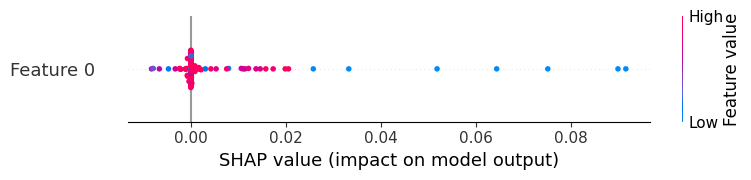
\includegraphics[width=0.4\textwidth]{shap/pos1.png}
        \caption{shap for Stacked LSTM on normal data}
        \label{fig:image1}
    \end{figure}%

\begin{figure}
        \centering
        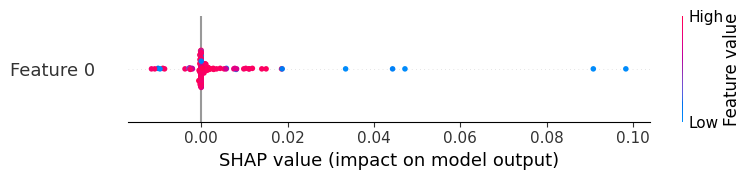
\includegraphics[width=0.4\textwidth]{shap/pos3.png}
        \caption{shap for CNN LSTM on normal data}
        \label{fig:image1}
    \end{figure}%

\begin{figure}
        \centering
        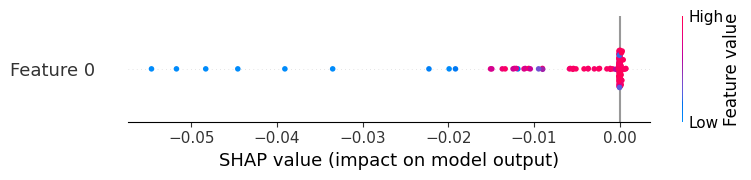
\includegraphics[width=0.4\textwidth]{shap/neg1.png}
        \caption{shap for Stacked LSTM on abnormal data}
        \label{fig:image1}
    \end{figure}%


\begin{figure}
        \centering
        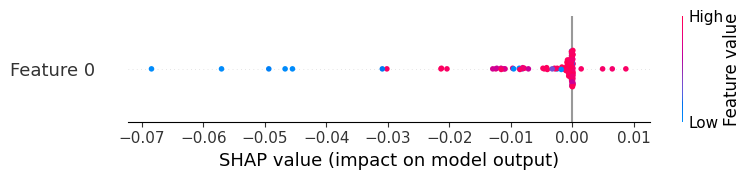
\includegraphics[width=0.4\textwidth]{shap/neg3.png}
        \caption{shap for CNN LSTM on abnormal data}
        \label{fig:image1}
    \end{figure}%
\subsubsection{\textbf{Observations for Abormal ECG Data}} High feature value of  abnormal data has low negative impact on model behavior. In contrast, Low feature value of  normal data has large negative impact on model behavior.
\subsection{\textbf{SHAP Subgroup Analysis on MIT-BIH}}
We are asked to find some demographic information like age, ethnicity etc in the MIT-BIH dataset and to do the SHAP subgroup analysis. Unfortunately, there is no demographic information in the mentioned dataset.Either .hea or .atr files were supposed to contain these type of information. But they only have info about the ECG data like .dat file.

\subsection{Challenges}
\begin{itemize}
    \item \textbf{Hardware Limitation}: Powerful GPUs are essential for faster processing.
    \item \textbf{Data Quality and Availability}: ECG data is often noisy, and the availability of balanced, labeled, and sufficient datasets is crucial.
    \item \textbf{Model Complexity}: LSTM networks are inherently complex and require careful tuning of hyperparameters to prevent overfitting or underfitting. Balancing reconstruction loss and classification accuracy presents significant challenges.
    \item \textbf{Training Time}: Training LSTMs and other deep learning models can be time-consuming, necessitating significant resources and patience for convergence.
    \item \textbf{Interpretability}: LSTMs and other deep learning models function as "black boxes," which complicates the interpretation of decision-making processes.
\end{itemize}

\section{Conclusion}
\subsection{Summary}
\subsubsection{\textbf{Short Intoduction}}
The project focused on the classification of electrocardiogram (ECG) signals using various architectures of Long Short-Term Memory (LSTM) networks, particularly leveraging autoencoders.

\subsubsection{\textbf{Datasets Used}}
\begin{itemize}
    \item \textbf{ECG5000}: This dataset consists of 5,000 ECG recordings, each containing 140 samples, making it suitable for time-series analysis and classification tasks.
    \item \textbf{MIT-BIH Arrhythmia Database}: A benchmark dataset widely used for evaluating algorithms aimed at detecting various types of arrhythmias.
\end{itemize}

\subsubsection{\textbf{Methodology}}
The project implemented several variations of LSTM architectures to classify ECG signals effectively. The following models were explored:
\begin{itemize}
    \item \textbf{Standard LSTM}: This model served as the baseline for comparison against more complex architectures.
    \item \textbf{Bidirectional LSTM (BiLSTM)}: This model processes the sequence data in both forward and backward directions, allowing it to capture context from both ends of the input sequence.
    \item \textbf{Stacked LSTM}: This architecture consists of multiple LSTM layers stacked on top of each other, enhancing the model's capacity to learn complex patterns in the data.
    \item \textbf{Convolutional LSTM (CNN-LSTM)}: This hybrid model combines convolutional layers with LSTM layers, enabling it to extract spatial features from the ECG signals before temporal analysis.
    \item \textbf{Inception LSTM}: Inspired by Inception networks in image processing, this architecture utilizes multiple filter sizes to capture various features from the input data.
\end{itemize}
\subsubsection{\textbf{Model evaluation Metrics}}
\begin{itemize}
    \item \textbf{Accuracy}:proportion of true results among the total number of cases 
    \item \textbf{Macro-F1}: harmonic mean of precision and recall
    \item \textbf{Precision}: ratio of true positive predictions to the total predicted positives
    \item \textbf{Recall}: ratio of true positive predictions to all actual positives
    \item \textbf{AUROC}: quantifies the ability of a binary classifier to distinguish between positive and negative classes
\end{itemize}

Each model was trained on both datasets, and their performances were evaluated based on accuracy and F1-score metrics.
\subsubsection{\textbf{SHAP Analysis}}
After training the models, SHAP (SHapley Additive exPlanations) analysis was conducted on the ECG5000 dataset. This technique provides insights into the contribution of each feature to the model's predictions, helping to interpret which aspects of the ECG signals are most influential in determining classifications. The SHAP analysis revealed that certain features related to heart rhythm patterns significantly impacted classification outcomes, thus enhancing model interpretability.

\subsubsection{\textbf{Results}}
The results indicated that hybrid models like CNN-LSTM and Inception LSTM outperformed standard LSTMs in terms of accuracy and robustness against noise in the data. The stacked LSTM also showed promising results but required more computational resources. The SHAP analysis further emphasized the importance of specific features, guiding future improvements in model design and feature engineering.

\subsection{Future Directions}
To build upon this work and enhance ECG classification further, several avenues can be explored:
\begin{itemize}
    \item \textbf{Integration with Other Modalities}: Combining ECG data with other physiological signals (e.g., blood pressure or respiratory rate) could provide a more comprehensive understanding of cardiac health.
    \item \textbf{Real-Time Monitoring Systems}: Developing real-time systems for continuous monitoring using wearable devices could facilitate early detection of arrhythmias.
    \item \textbf{Transfer Learning}: Applying transfer learning techniques from related domains could improve model performance, especially with limited labeled data.
    \item \textbf{Advanced Feature Extraction Techniques}: Exploring methods like wavelet transforms or deep learning-based feature extraction could enhance input representation for better classification.
    \item \textbf{Ensemble Learning Approaches}: Implementing ensemble methods that combine predictions from multiple models may yield improved accuracy and robustness against overfitting.
    \item \textbf{Explainable AI Methods}: Further research into explainable AI techniques can enhance trust in model predictions, particularly important in clinical settings where decisions can directly affect patient outcomes.
\end{itemize}

This project not only contributes to advancements in ECG classification but also lays a foundation for future research aimed at improving cardiac health monitoring through machine learning technologies.






\bibliographystyle{ACM-Reference-Format}
  \bibliography{ref}
\end{document}

